%% An Introduction to LaTeX Thesis Template of Wuhan University
%%
%% Created by WHUTUG

\documentclass{whu-thesis}
\whusetup
  {
    info               =
      {
        title          = {基于连续时间的LiDAR/Camera/IMU的时空标定方法},
        title*         = {Continuous-time based spatio-temporal calibration method for LiDAR/Camera/IMU},
        student-number = {2019302141103},
        school         = {测绘学院},
        author         = {陈烁龙},
        author*        = {Your Name},
        subject        = {学科},
        major          = {测绘工程},
        advisor        = {李星星 , 教授},
        direction      = {研究方向},
        % date           = {2021/5},
        keywords       = {连续时间,多传感器系统,时空标定,因子图优化,可观性分析},
        keywords*      = {continuous-time, multi-sensor system, temporal-spatial calibration, factor graph optimization, observability analysis},
      },
    style              =
      {
        graphics-path  = {{figures/}{data/}},
        list-of-figures,
        list-of-tables,
      },
    element            =
      {
        innovation     = {pages/innovation},
        abstract       = {pages/abstract},
        abstract*      = {pages/enabstract},
        bibliography   = {ref/refs , ref/thu},
        achievements   = {pages/achievements},
        thanks         = {pages/thanks},
        appendix       = {pages/appendix}
      }
  }

\usepackage{multirow}
\usepackage{amsmath, listings, fontspec, geometry, graphicx, color, amsfonts, amssymb}

\newcommand\normf{}
\newcommand\liehat[1]{\left[ #1 \right]_\times}
\newcommand\lievee[1]{\left[ #1 \right]^\vee}
\newcommand\liehatvee[1]{\left[ #1 \right]^\vee_\times}

\newcommand\mlcomment[1]{\iffalse #1 \fi}
% \newcommand\mlcomment[1]{ #1 }

\begin{document}
%%----------- 主体部分 ----------- %%
% Chapter 1

\chapter{\normf{绪论}}
\normf
近年来,随着自动驾驶、服务机器人等智能技术的发展,位置服务和场景感知变得越来越重要。比如,智能车辆在行进过程中,需要进行连续、可靠 、无缝的高精度定位;机器人在运作过程中,需要进行实时定位和建图,同时感知周围的环境。对于简单的应用场景,单一传感器即可胜任上述工作。但在复杂场景下,基于单一传感器的技术存在局限性,无法满足上述需求,往往需要通过多传感器融合技术来实现。以无人车为例,在城市峡谷、隧道等复杂场景下,基于单一传感器的技术很难为无人车提供连续、可靠的定位,而通过多传感器的融合即可以达到这一需求;在人流、车流密集的城市内部道路中,无人车需要对周边复杂的场景进行感知以作出相应的决策,对此单一传感器无法胜任,需要通过多个传感器配合来实现。相较于单一传感器系统,多传感器组合系统能够发挥不同传感器之间的互补特性,在复杂场景中提供更优的服务。但是,多传感器组合系统需要额外进行多传感器之间相关参数的标定,且参数标定的精确程度直接影响着算法实现高精度定位或精准场景感知的能力。

多传感器标定算法因传感器类型而异。目前在自动驾驶和智能机器人领域,使用得较多的传感器是LiDAR、Camera和IMU,它们都能独立地提供载体相对于参考坐标系的位姿信息,且存在各自的优势和不足,因此常常通过融合算法组合使用。相应的,也就需要对组合系统涉及的多个传感器进行标定。基于这一点,本章先对涉及上述三类传感器的多传感器标定算法的研究现状和发展趋势进行分析,而后引出本文的具体研究内容。

\section{\normf{研究背景与意义}}
就位置服务而言,在目前存在的各种定位技术中,全球卫星导航系统(Global Navigation Satellite System,GNSS)无疑是应用得最为广泛的全局定位技术,其能够在全球范围和近地表面提供全天候、全天时的定位服务。但是,GNSS技术作为一种基于无线电信号的导航定位技术,在诸如城市峡谷、隧道、室内等信号易受遮蔽和干扰的复杂场景中,其定位精度会有所下降,甚至完全失效\cite{li2023multi}。

相较于易受外界环境干扰的GNSS技术,基于惯性测量单元(Inertial Measurement Unit,IMU)实现的惯性导航系统(Inertial Navigation System,INS)不受环境的干扰,能够通过连续积分实现相对定位,具有高频、自主、无源的优点,但是受测量噪声和零偏的影响,其不可避免地存在误差发散问题。因此在车载导航中,常常将两者结合使用,利用GNSS提供的全局定位信息抑制INS的误差发散,同时在复杂环境中通过INS辅助GNSS定位,以提供更加连续、可靠的位置服务\cite{titterton2004strapdown}。IMU除了在车载导航中被广泛使用外,其作为一种高频、低功耗的内部传感器,在近年来不断发展的诸如增强现实(Augmented Reality,AR)、智能机器人等新兴技术领域,也有着较大的应用潜能。

相较于IMU这种内部传感器,Camera、LiDAR等外部传感器可以在提供载体位姿的同时感知周围的环境,因此被广泛应用于自动驾驶和智能移动机器人领域。Camera可以对周围场景连续地获取二维影像。基于所获取影像的几何特征和光度信息,载体可以在实现定位定姿的同时,完成场景的识别、扫描和重建。但是,相机在成像过程中将外部的三维场景映射到二维影像平面上,导致了场景深度信息的缺失。因此对于单目相机而言,即使通过相应的算法恢复了场景结构,其尺度也是未知的。为了恢复尺度,可以通过组合多个相机来实现,也可以通过结合LiDAR这种带有尺度的传感器来达到。相较于Camera,LiDAR能够直接感知周围环境的距离和方位信息,但无法获取场景的纹理信息。因此可以将LiDAR和Camera结合使用,以充分发挥两类传感器之间的互补特性,实现更为鲁棒的相对位姿估计和场景重建。同样的,IMU也可以辅助Camera和LiDAR,进行特征跟踪和畸变消除,同时提供相对位姿约束。

总的来说,多传感器融合作为一种解决复杂问题的有效手段,在位置服务、场景感知或是其他智能服务领域都被广泛地使用。但是相应的,也需要进行额外的多传感器标定工作。对于大多数的多传感器融合算法而言,多传感器系统被正确地标定是实现精确的运动估计或有效的场景感知的前提。相比于只需关注传感器内参的单传感器算法,多传感器算法为了融合来自不同传感器的量测信息,需要考虑各传感器之间的外参。另外,粗糙的时钟同步、不精确的硬件触发以及传输延迟,也会导致系统的不稳定或状态估计不准确,因此与时间相关的参数也需要校准\cite{yang2019degenerate}。特别的,对于卷帘快门相机(Rolling Shutter,RS)而言,由于其以单行扫描的方式进行图像采集,不同像素行之间存在时差。在动态场景下,这会导致图像受果冻效应的影响,因此与此相关的时间参数也需要被标定。

基于上述需求,本文提出了一个基于连续时间(Continuous Time,CT)的无靶标多传感器时空标定框架,并基于LiDAR/Camera/IMU组合系统对其进行了实现。相较于基于离散时间(Discrete Time,DT)的标定方法,其将时参严密纳入到最优化问题中进行求解。该标定框架具有易操作性、可扩展性和鲁棒性,对于多传感器融合算法的研制和相关智能服务设施的正真落地有着重要的实际意义和应用价值。

\section{\normf{国内外研究现状和发展趋势}}

\subsection{\normf{Camera/IMU方面}}
Camera/IMU组合系统使用的是低成本、低功耗的Camera和IMU。Camera可以连续地获取场景的灰度影像,能够在提供较高精度相对位姿的同时恢复出场景的三维结构;IMU可以连续、高频地输出载体相对于惯性坐标系的线加速度和角速度,能够为Camera的相对位姿估计提供预积分量测(Pre-Integration Measurement,PIM)约束\cite{qin2018vins},或者在视觉失效的场景下能够连续独立地输出载体的相对位姿信息。因此诸如视觉惯性里程计(Visual Inertial Odometry,VIO)、视觉辅助的惯性导航系统(Vision-aided Inertial Navigation Systems,VINS)等Camera/IMU组合系统在增强现实、智能机器人、文物保护和考古等领域有着较为广泛的应用。而且出于成本的考虑,这些部署在诸如智能手机、扫地机器人等智能设备上的Camera/IMU组合系统一般配备的都是价格低廉的Camera和MEMS级别的IMU,在出厂时传感器相关参数的标定都较为粗略,且到消费者手中后几乎不可能进行二次标定(尤其是基于有靶标的标定方法),显然这会严重损害相关算法的精度。为此,Huai等\cite{huai2022observability}基于滤波方法实现了一个能够进行在线自标定的VIO系统,并对系统的可观性进行了分析。该方法在标定过程中同时考虑了传感器的内参、外参和时参,是一个基于自运动进行无靶标标定的方法。Mirzaei等\cite{mirzaei2008kalman}基于迭代扩展卡尔曼滤波器(Iterated Extended Kalman Filter,IEKF),实现了一个事后的Camera/IMU标定系统,但是其需要通过标定板初始化相机的位姿序列,是一种有靶标的标定方法。另外,该方法需要通过CAD或人为量测来给定待标参数较为精确的初值,而这在实际操作中难以保证,因此其应用受较大程度上的限制。与此类似,Yang等\cite{yang2019degenerate}基于多状态约束下的卡尔曼滤波器(Multi-State Constraint Kalman Filter,MSCKF)实现了一个Camera/IMU标定系统,并在理论层面考察了不同形式的退化运动对系统可观性的影响。

上述基于滤波的标定方法都依托离散时间估计理论对待标参数进行估计,在处理传感器异步测量值时需要将所有状态递推到测量时刻,且当涉及时参估计时,该问题会变得更为严峻。相反的,连续时间估计理论通过构建时间连续函数,将时参纳入到严密的估计系统中,在处理传感器异步测量值时,只需要进行简单的时间采样(Sampling)或查询(Querying),即可获得对应的系统状态。Furgale等\cite{furgale2013unified}基于连续时间估计理论,使用B样条曲线建模IMU的位姿和零偏,实现了一个基于图优化估计的Camera/IMU标定系统。该方法将Camera和IMU之间的时延参数纳入到因子图中进行估计,在给定较为精确的传感器量测模型下,能够获得较高精度的估值。但是,该方法需要通过标定板初始化相机的位姿序列,也同样需要较为精确的外参初值,以基于初始化的相机位姿序列恢复出初始的IMU位姿序列。之后,他们将激光雷达也纳入到该系统中进行标定\cite{rehder2014spatio}。

由上文可知,当前的Camera/IMU标定方法大部分基于离散时间估计,通过滤波方法进行实现。在涉及时参估计时,该类方法实现的系统的复杂度将会大大增加,同时性能会降低。而基于连续时间估计,通过图优化方法实现的标定方法则能较好的处理时参估计问题。且由于使用图优化进行参数估计,此类标定方法往往需要一个初始化的步骤来提供待估参数的初值,但目前大部分的标定系统的初始化不是自动完成的,而是通过手动赋值或者靶标辅助的方式进行,这在大多数情况下是不能满足的。

\subsection{\normf{LiDAR/IMU方面}}
LiDAR/IMU组合系统使用的传感器为激光雷达(Light Detection and Ranging,LiDAR)和IMU。与Camera单帧只能获取场景在像平面上的二维投影不同,LiDAR单帧可以直接获取场景的三维信息。为了重构完整的场景,Camera需要利用相机影像序列构建多视图几何问题,并耗费大量计算资源来求解方程组,且对于单目相机而言,场景的尺度是未知的。而LiDAR只需要进行简单的帧到帧或者帧到地图匹配即可得到带有尺度的场景点云地图。在位姿估计方面,Camera需要基于特征点法或者光流法,通过共视图构建优化问题求解,且由于相机量测模型稍复杂,因此优化问题的非线性较严重\cite{高翔2017视觉}。而LiDAR的量测模型简单,通过匹配即可获得高精度的相对位姿。由于LiDAR能够在输出高精度的相对位姿信息的同时提供高精度的稠密点云地图,因此其在自动驾驶领域颇受欢迎。但在成本方面,LiDAR相较于Camera存在劣势,且会受到运动畸变的影响。对于LiDAR的运动畸变,VICP方法\cite{hong2010vicp}假设运动为匀速运动,在匹配的同时估计LiDAR的速度以去除畸变的影响,但是在低采样频率情况下匀速运动假设很难成立。另一种更常用的方法是使用IMU辅助,基于IMU输出的高频角速度和线加速度信息来进行畸变去除\cite{shan2020lio}。另外,基于IMU输出构建的PIM可以为LiDAR匹配提供更好的初值和更强的约束。因此诸如雷达惯性里程计(Lidar Inertial Odometry,LIO)等的LiDAR/IMU组合系统相较于单LiDAR系统,应用更为广泛。相应的,LiDAR/IMU组合系统的标定也成为了一个问题。Liu等\cite{liu2019novel}基于卡尔曼滤波器(Extended Kalman Filter,EKF)方法,通过提取环境中的球特征、圆柱特征和面特征构建约束,实现了一个无靶标的LiDAR/IMU标定系统。但是,该方法需要使用精确的控制平台来驱动IMU,因此使用受到极大的限制,尤其是在机器人领域。而且该方法使用离散时间估计,标定过程中只考虑了LiDAR/IMU组合系统的内外参数,不涉及时参。

如前文所述,Rehder等\cite{rehder2014spatio}在基于连续时间估计的Cmaera/IMU标定系统\cite{furgale2013unified}基础上引入了激光雷达,提出了一个LiDAR/Camera/IMU组合系统的两步标定方法。该方法在进行LiDAR/IMU标定时,通过面特征构建点到面约束进行参数优化,能够同时估计内外参和时参,但是需要较好的外参初值。Li等\cite{li20213d}同样基于连续时间估计,通过高斯过程(Gaussian Process,GP)建模IMU位姿轨迹,实现了一个无靶标的LiDAR/IMU标定系统。由于加入了初始化模块,其不要参数初值的给定。但是该方法需要事先通过地面激光扫描仪(Terrestrial Laser Scanner,TLS)获取一个稠密的先验点云地图,用以构建点到面关联,而这在实际使用时很难保证。Lv等\cite{lv2020targetless}通过雷达里程计初始化点云地图,并基于B样条曲线构建IMU的位姿轨迹,实现了一个无需靶标的LiDAR/IMU组合系统时空标定框架。且该方法精细设计了一个初始化模块,因此不要事先给定参数初值。之后,他们在可观性感知方面对系统做了进一步优化,使系统在标定时启发式地选择富含信息量的数据片段参与运算,以在不影响标定精度的前提下提高系统的运算效率\cite{lv2022observability}。

如上文所述,目前在LiDAR/IMU系统的标定方面,大部分方法是采用无靶标的方式进行,通过提取环境特征构建约束来求解待估参数。但是,在特征提取和约束构建方面仍然存在一定的问题,大部分方法在一般场景下很难提取到稳健的环境特征来构建约束。另外,基于图优化进行参数估计的标定方法的初始化步骤仍然值得讨论和改进。

\subsection{\normf{Camera/LiDAR方面}}
Camera/LiDAR组合系统使用的传感器为Camera和LiDAR,二者均属于外部传感器。LiDAR能够直接获取周围场景的点云量测信息,这是相机不能做到的;相机可以获取场景的纹理、色彩和表面信息,这是LiDAR不能做到的。由于二者存在较好的互补特性,因此该组合被广泛应用于移动机器人、自动驾驶等领域。如在场景重建方面,Camera/LiDAR组合可以重建出带有纹理的三维场景;在目标检测方面,基于相机拍摄的影像,可以通过识别算法定位目标方向,而后结合LiDAR帧可以快速锁定目标位置。事实上,目前已有RGBD相机实现了类似于Camera/LiDAR组合系统的功能,但是其视场角小,有效测程短,很难在大尺度的场景中发挥作用\cite{高翔2017视觉}。对于Camera/LiDAR组合系统的标定而言,目前提出的方法大多通过关联相机帧和LiDAR帧中的特征构建约束,而后将约束和待标参数一同加入到优化问题中进行求解。Park等\cite{park2014calibration}使用一个多边形平板作为靶标,通过在LiDAR帧和相机帧中分别提取平板顶点,而后构建点到点关联约束求解外参。Li等\cite{li2022accurate}基于自制的带孔棋盘平板,在LiDAR帧和相机帧中估计圆孔中心,而后同样构建点到点关联约束进行求解。该标定方法支持多种常见的LiDAR传感器。

以上所提到的方法均是基于人工靶标实现的系统外参标定。对此,Mishra等\cite{mishra2020experimental}对几种比较典型的基于人工靶标的Camera/LiDAR组合系统的标定方法进行了测试。相比于基于人工靶标的标定方法,基于特征的标定方法利用环境信息构建关联约束进行标定参数的求解,其不需要额外的靶标进行辅助,具有更好的适用性。Yuan等\cite{yuan2021pixel}通过提取环境中的深度连续线特征构建关联关系,实现了Camera/LiDAR组合系统外参的无靶标标定。为了能够精确提取到LiDAR帧中的线特征,该方法需要通过Livox类型的固态雷达静态采集一段时间的数据,以获取较为稠密的点云。Gong等\cite{gong20133d}基于环境中较为常见的三面相交特征提取特征面,结合自运动估计方法构建非线性最小二乘问题进行系统外参的无靶标标定。这些方法都是基于离散时间估计的标定方法,在标定过程中都没有考虑时延参数的估计。Park等\cite{park2020spatiotemporal}基于连续时间估计,通过构造投影因子优化求解LiDAR和Camera时间的外参和时延参数,同样是一种基于自运动的无靶标标定方法。但是其使用简单的一阶内插来构建时间连续轨迹,当载体充分激励运动时会引入较大的偏差(基于自运动的标定方法往往需要运动被充分激励来保证待估参数的精度)。

上文所诉的标定方法虽然都能达到比较好的外参标定精度,但是除\cite{park2020spatiotemporal}外都是静态标定,没有考虑时参,而这对于一个多传感器组合系统是不容忽视的。特别是在高动态场景下,未进行严格的时间同步会造成算法精度的损失,这是不能接受的。

\section{\normf{研究内容及论文总体安排}}

\subsection{\normf{研究内容}}
围绕上述多传感器标定方面的研究现状和发展趋势,本文的研究内容如下:
\begin{enumerate}
    \item 基于连续时间的LiDAR/Camera/IMU的时空标定方法的设计与实现
    
    从连续时间估计理论出发,依托IMU的输出构造位姿B样条曲线,基于多传感器原始观测值构建约束,通过因子图优化方法迭代求解待标定的时空参数(内参、外参、时参),逐步达到系统的全局最优。

    \item 基于连续时间的LiDAR/Camera/IMU的时空标定方法的验证与评价
    
    基于虚拟实验平台构建仿真场景,对所提出的标定框架的可行性进行验证。同时基于自主搭建的实验平台,在室内外典型场景下进行实测实验,对所提出的标定框架进行综合的测试和评估。最后对算法的一致性进行评价。
    
    \item 基于连续时间的LiDAR/Camera/IMU的时空标定方法的系统可观性分析和验证
    
    从LM方法的增量方程出发,通过考察方程系数矩阵的零空间,对不同形式退化运动下的系统待标参数的可观性进行了理论分析。同时通过虚拟实验平台构建模拟轨迹,对系统可观性的理论分析进行验证。
    
\end{enumerate}

\subsection{\normf{章节安排}}

第一章为绪论部分,介绍了多传感器标定的背景与意义,以及目前国内外的研究现状和发展趋势。其中,着重分析了当前针对Camera/IMU、LiDAR/IMU和Camera/LiDAR等多传感器系统的标定算法的特点和局限性,并对本文所研究的基于连续时间的LiDAR/Camera/IMU的时空标定方法进行了必要性分析。

第二章为多传感器标定的基础。本章首先介绍了本文的标定方法涉及的坐标系,以及坐标系之间的刚体变换,接着介绍了LiDAR、Camera、IMU的传感器模型。由于本文研究的是基于连续时间的标定算法,因此本章对连续时间理论也进行了相应的介绍。最后对图优化理论进行了介绍。

第三章详细介绍了本文所提出的基于连续时间的LiDAR/Camera/IMU的时空标定方法。本章首先对整个系统的算法框架和状态定义进行了阐述,而后依据算法框架的处理流程,依次介绍了系统的初始化、数据关联和批处理优化。

第四章对实验部分进行了阐述和分析。在本章中,首先基于仿真实验平台GAZEBO模拟的数据,对所提出的标定框架的可行性进行了验证。而后基于自主搭建的实验平台,在室内外两种不同的典型场景下进行了实测实验,对所提出的基于连续时间的LiDAR/Camera/IMU的时空标定方法进行综合的测试和评估。最后,针对不同类型的退化运动,对系统可观性进行了理论分析和实验验证。

第五章为总结与展望。本章首先基于所提出的多传感器标定算法框架,对当前所完成的工作进行了总结归纳,接着对后续可开展的工作进行了展望。


% Chapter 2

\chapter{\normf{理论基础}}
本文所研究的多传感器标定算法是一种基于自运动的时空参数标定方法,其基于连续时间理论,通过因子图优化的方式估计待标参数。因此,在介绍算法之前,有必要进行相关理论的阐述和相关符号的说明。

\section{\normf{坐标系定义}}
本文提出的标定方法涉及内参、外参和时参,其中描述不同传感器坐标系之间相对位姿关系的外参是较为重要的一部分,其涉及到了传感器坐标系的表示。本文所研究的算法涉及LiDAR、Camera和IMU这三种传感器,下面依次给出各传感器坐标系的定义。
\begin{enumerate}
  \item LiDAR坐标系

        LiDAR坐标系以激光脉冲发射中心作为原点,其Y轴指向正前方,Z轴指向天顶方向,X轴与Y轴和Z轴构成右手直角坐标系。本文用字母$L$表示LiDAR坐标系,用花体字母$\mathcal{L}$表示LiDAR坐标系序列,用$L_i$表示序列中的第$i$个LiDAR坐标系,其中$i\in\mathcal{L}^\dagger$。符号$(\cdot)^\dagger$表示对序列集合元素取标号的操作。
  \item Camera坐标系

        Camera坐标系以相机光心作为原点,其Z轴指向正前方(即相机主光轴方向),X轴垂直于Z轴向右,Y轴与X轴和Z轴构成右手直角坐标系,指向天顶方向的反方向。本文用字母$C$表示Camera坐标系,用花体字母$\mathcal{C}$表示Camera坐标系序列,用$C_j$表示序列中的第$j$个Camera坐标系,其中$j\in\mathcal{C}^\dagger$。
  \item IMU坐标系

        IMU是由加速度计和陀螺仪两种器件构成,安装时二者的坐标系可能不一致\footnote{\normf{该偏差被称为IMU安装误差(IMU Misalignment)。在本标定算法中会考虑这个偏差,详细内容见\ref{sensro_model_imu}节。}}。在本文中,将加速度计坐标系视为IMU坐标系,即在加速度计不存在交轴耦合误差\footnote{\normf{指三个轴不严格正交,详细内容见\ref{sensro_model_imu}节。}}(Axis Misalignment)的前提下,IMU坐标系的三个正交轴和加速度计坐标系的轴向完全重合。IMU坐标系也是一个右手直角坐标系,本文用字母$I$表示该坐标系,用字母$A$、$G$表示加速度计和陀螺仪的坐标系,用花体字母$\mathcal{I}$表示IMU坐标系序列,用$I_k$表示序列中的第$k$个IMU坐标系,其中$k\in\mathcal{I}^\dagger$。
\end{enumerate}
\section{\normf{坐标系刚体变换}}
三维刚体变换(Rigid Body Transformation)描述了三维空间中两个刚体坐标系之间的相对位姿关系,其由姿态量和平移量构成,存在6个自由度,具有多种数学表达形式。下面对常用的几种表达形式进行阐述。
\subsection{\normf{变换矩阵}}
变换矩阵(Transform Matrix)由旋转矩阵和平移向量构成,通过下式定义:
\begin{equation}
  \boldsymbol{T}=\begin{pmatrix}
    \boldsymbol{R} & \boldsymbol{p} \\\boldsymbol{0}&1
  \end{pmatrix}\in\mathrm{SE(3)}\quad \mathrm{s.t.}\quad\boldsymbol{R}\in \mathrm{SO(3)},\;\boldsymbol{p}\in \mathbb{R}^3
\end{equation}
其中:$\boldsymbol{R}$为旋转矩阵,其存在于三维空间中的特殊正交群SO(3)中,同时也是一个单位正交阵\footnote{\normf{即旋转矩阵满足$\boldsymbol{R}\boldsymbol{R}^T=\boldsymbol{I},\det\boldsymbol{R}=1$。}};$\boldsymbol{p}$是三维的平移向量;$\boldsymbol{T}$即为变换矩阵,其存在于三维空间中的特殊欧式群SE(3)中。对于自由度为6的三维刚体变换而言,变换矩阵是冗余的,不是最小表达形式。
\subsection{\normf{欧拉角和轴角}}
欧拉角(Euler Angles)使用三个绕正交轴旋转的角来表示姿态,结合平移向量,同样可以表达三维刚体变换。对于一次刚体旋转,可以将其分解为三次绕轴旋转的角,相应的,也可以通过依次绕指定轴旋转相应的角度恢复出刚体旋转。欧拉角与绕轴旋转的顺序相关,顺序不同,结果也会不同。其中最为常用的是“翻滚-俯仰-航偏”(roll-pitch-yaw)的欧拉角,即rpy角。欧拉角是三维刚体旋转的最小表达形式,且较为直观,但存在万向锁问题(Gimbal Lock),会导致旋转奇异。如对于rpy角而言,当俯仰角为$\pm \pi/2$时,翻滚角和航偏角绕空间中的同一个轴旋转,导致一个自由度的丢失。

另外,刚体旋转也可以直接表示为绕空间某个轴旋转一个角的形式,该种表达形式被称为轴角(Axis Angle)或者旋转向量。轴角一般用向量$\boldsymbol{\theta}\in\mathbb{R}^3$表示,向量的指向即为旋转轴的方向,向量的模长即为旋转角度的大小。轴角同样也是三维刚体旋转的最小表达形式。

\subsection{\normf{单位四元数}}
单位四元数(Unit Quaternion)用一个实数和三个虚数构成的四维单位向量表示旋转,相比欧拉角多了一个自由度\footnote{\normf{相对应的,也多了一个约束,即模长为单位1。}},但是不存在奇异问题,是一种紧凑的表达形式。单位四元数的定义如下:
\begin{equation}
  \boldsymbol{q}=q_w+q_x\boldsymbol{i}+q_y\boldsymbol{j}+q_z\boldsymbol{k}\quad \mathrm{s.t.}\quad
  \begin{cases}
    \boldsymbol{i}^2=\boldsymbol{j}^2=\boldsymbol{k}^2=-1                                                                                       \\
    \boldsymbol{i}\boldsymbol{j}=\boldsymbol{k}\quad\boldsymbol{j}\boldsymbol{k}=\boldsymbol{i}\quad\boldsymbol{k}\boldsymbol{i}=\boldsymbol{j} \\
    q_w^2+q_x^2+q_y^2+q_z^2=1^2
  \end{cases}
\end{equation}
其中$\boldsymbol{i}$、$\boldsymbol{j}$、$\boldsymbol{k}$为虚数单位。单位四元数可以表示成显含轴角的形式:
\begin{equation}
  \boldsymbol{q}=\cos\frac{\Vert \boldsymbol{\theta}\Vert}{2}+\frac{\boldsymbol{\theta}}{\Vert \boldsymbol{\theta}\Vert}\sin\frac{\Vert \boldsymbol{\theta}\Vert}{2}
\end{equation}
\subsection{\normf{李代数}}
三维刚体变换的另一种最小表示是李代数(Lie Algebra)。与旋转矩阵$\boldsymbol{R}$在流形(Manifold)上表示旋转不同,姿态李代数$\boldsymbol{\liehat{\boldsymbol{\phi}}}\in\mathfrak{so}(3)$在正切空间(Tangent Space)表示旋转,因此当涉及优化问题中的雅克比矩阵求解和状态增量更新时较为简洁便利(具体见附录\ref{appendix:lie_alg_update})。其中$\liehat{\cdot}$表示将三维向量映射为反对称矩阵,与此对应的$\lievee{\cdot}$则将反对称矩阵映射为三维向量,即:
\begin{equation}
  \boldsymbol{\phi}=\begin{pmatrix}
    \phi_x \\\phi_y\\\phi_z
  \end{pmatrix}\in\mathbb{R}^3 \quad
  \liehat{\boldsymbol{\phi}}=\begin{pmatrix}
    0       & -\phi_z & \phi_y  \\
    \phi_z  & 0       & -\phi_x \\
    -\phi_y & \phi_x  & 0       \\
  \end{pmatrix}\quad \liehatvee{\boldsymbol{\phi}}=\boldsymbol{\phi}
\end{equation}

姿态李代数$\boldsymbol{\liehat{\boldsymbol{\phi}}}$和旋转矩阵$\boldsymbol{R}$之间的转换可以通过指数映射和对数映射实现:
\begin{equation}
  \boldsymbol{R}=\exp(\liehat{\boldsymbol{\phi}}) \quad \liehat{\boldsymbol{\phi}}=\log(\boldsymbol{R})
\end{equation}
而首字母大写的指数映射和对数映射,则可直接建立姿态李代数向量$\boldsymbol{\phi}$和旋转矩阵$\boldsymbol{R}$之间的关系:
\begin{equation}
  \boldsymbol{R}=\mathrm{Exp}(\boldsymbol{\phi}) \quad \boldsymbol{\phi}=\mathrm{Log}(\boldsymbol{R})
\end{equation}
除了可以建立SO(3)和$\mathfrak{so}(3)$之间的映射外,还存在SE(3)和$\mathfrak{se}(3)$之间的映射,后者使用6维向量同时表达姿态量和位移量,这里不再介绍,具体可参考\cite{sola2018micro}。

\subsection{\normf{坐标系变换}}
假设空间中存在两个坐标系$F_i$、$F_j$,以及点$\boldsymbol{p}$和向量$\boldsymbol{v}$,则将点或向量从$F_i$系变换到$F_j$系的过程,可以等价表达为如表\ref{tab:rbt}所示的不同形式。
\begin{table*}[htbp]
  \centering
  \caption{\normf{点和向量坐标系变换的不同表达形式}}
  \label{tab:rbt}
  \begin{tabular}{c|c|c|c|c}
    \hline
    \normf{对象}             & \normf{${^{j}_{i}}\boldsymbol{T}$}                          & \normf{${^{j}_{i}}\boldsymbol{R}$和${^{j}\boldsymbol{p}_{i}}$} & \normf{${^{j}_{i}}\boldsymbol{q}$和${^{j}\boldsymbol{p}_{i}}$} & \normf{${^{j}_{i}}\boldsymbol{\phi}$和${^{j}\boldsymbol{p}_{i}}$} \\ \hline
                             &                                                             &                                                                &                                                                &                                                                   \\
    \normf{$\boldsymbol{p}$} & $\begin{pmatrix}
                                    {^{j}}\boldsymbol{p} \\1
                                  \end{pmatrix}={^{j}_{i}}\boldsymbol{T} \circ\begin{pmatrix}
                                                                                {^{i}}\boldsymbol{p} \\1
                                                                              \end{pmatrix}$
                             &
    ${^{j}}\boldsymbol{p}={^{\boldsymbol{j}}_{\boldsymbol{i}}}\boldsymbol{R}\circ{^{i}}\boldsymbol{p}+{^{j}\boldsymbol{p}_{i}}$
                             &
    ${^{j}}\boldsymbol{p}={^{\boldsymbol{j}}_{\boldsymbol{i}}}\boldsymbol{q}\circ{^{i}}\boldsymbol{p}+{^{j}\boldsymbol{p}_{i}}$
                             &
    ${^{j}}\boldsymbol{p}={^{\boldsymbol{j}}_{\boldsymbol{i}}}\boldsymbol{\phi}\circ{^{i}}\boldsymbol{p}+{^{j}\boldsymbol{p}_{i}}$                                                                                                                                                               \\ &&&&\\
    \normf{$\boldsymbol{v}$}
                             &
    $\begin{pmatrix}
         {^{j}}\boldsymbol{v} \\0
       \end{pmatrix}={^{j}_{i}}\boldsymbol{T} \circ\begin{pmatrix}
                                                     {^{i}}\boldsymbol{v} \\0
                                                   \end{pmatrix}$
                             &
    ${^{j}}\boldsymbol{v}={^{\boldsymbol{j}}_{\boldsymbol{i}}}\boldsymbol{R}\circ{^{i}}\boldsymbol{v}$
                             &
    ${^{j}}\boldsymbol{v}={^{\boldsymbol{j}}_{\boldsymbol{i}}}\boldsymbol{q}\circ{^{i}}\boldsymbol{v}$
                             &
    ${^{j}}\boldsymbol{v}={^{\boldsymbol{j}}_{\boldsymbol{i}}}\boldsymbol{\phi}\circ{^{i}}\boldsymbol{v}$                                                                                                                                                                                        \\
                             &                                                             &                                                                &                                                                &                                                                   \\
    \hline
  \end{tabular}
\end{table*}
\newline
其中:$\circ$表示相应的群运算、代数运算或矩阵运算,具体可参考文献\cite{sola2018micro};${^{i\mid j}}(\boldsymbol{p}\mid\boldsymbol{v})$表示点或向量在参考坐标系$F_{i\mid j}$系下的坐标表达。注意到,对于向量而言,变换坐标系只需考虑旋转量即可。在下文涉及坐标变换时,认为以上几种表达方式是等价的,且省略符号$\circ$的书写,不再具体说明。

\section{\normf{传感器模型及待标参数}}
本文所研究的算法涉及到了LiDAR、Camera和IMU这三种传感器,下面对各传感器模型进行阐述,并基于传感器模型给出本文标定算法框架中的待标参数。
\subsection{\normf{LiDAR}}
激光雷达(Light Detection and Ranging,LiDAR)向目标发射激光光束并接收回波信号,通过信号处理获取目标的相关信息,如距离,方位、反射率等,是一种外部传感器。激光雷达具有分辨率高、体积小、精度高等优点,被广泛应用于智能测绘、自动驾驶等领域。根据扫描方式的不同,激光雷达可分为机械式、固态式和混合固态式三种。由于本文研究的算法主要针对机械式激光雷达,故下面对其进行介绍。

机械式激光雷达在垂向上排布多个激光发射器(Laser Rangerfinder),在数据采集时通过不断地旋转发射器,实现三维场景的扫描。对于空间中探测到的一目标点$\boldsymbol{p}$,基于探测到的距离信息和激光光束的方向信息,可以得到该点在当前$L$系下的三维位置:
\begin{equation}
  \label{equ:lidar_model}
  {^{L}\boldsymbol{p}}=\begin{pmatrix}
    p_x \\
    p_y \\
    p_z
  \end{pmatrix}=\begin{pmatrix}
    d\times\cos\alpha\times\cos\beta \\
    d\times\cos\alpha\times\sin\beta \\
    d\times\sin\alpha
  \end{pmatrix}
\end{equation}
其中:$d$是$L$系坐标原点到点$\boldsymbol{p}$的直线距离,$\alpha$、$\beta$分别是激光光束在扫描点$\boldsymbol{p}$时的旋转角和高度角,如图\ref{fig:lidar_model}所示;${^{L}\boldsymbol{p}}$为点$\boldsymbol{p}$在当前$L$系下的坐标表达。机械式激光雷达发射器旋转一周,采集到的点的集合就构成一帧点云。如果机械式激光雷达采集数据时伴随有运动,则点云帧会存在运动畸变\footnote{\normf{因为在同一帧点云里,激光雷达采集每个点时L系不同,当通过归算,将一帧中的所有点表达到同一个L系下。}},如图\ref{fig:lidar_motion_distort}所示,因此需要进行去畸变处理。常用的去畸变方法有匀速模型、匀加速模型,或使用其他传感器辅助,如IMU。
%%%%%%%%%%%%%%%%%%%%%%%%%%%%%%%%%%%%%%%%%%%%%%%%%%%%%%%%%%%%%%%%%%%%%%%%%%%%%%%%%%%%%%%%%
\mlcomment{
  \begin{figure}[htbp]
    \centering

    % \subfigure[\normf{量测模型}]{
    %   \centering
    %   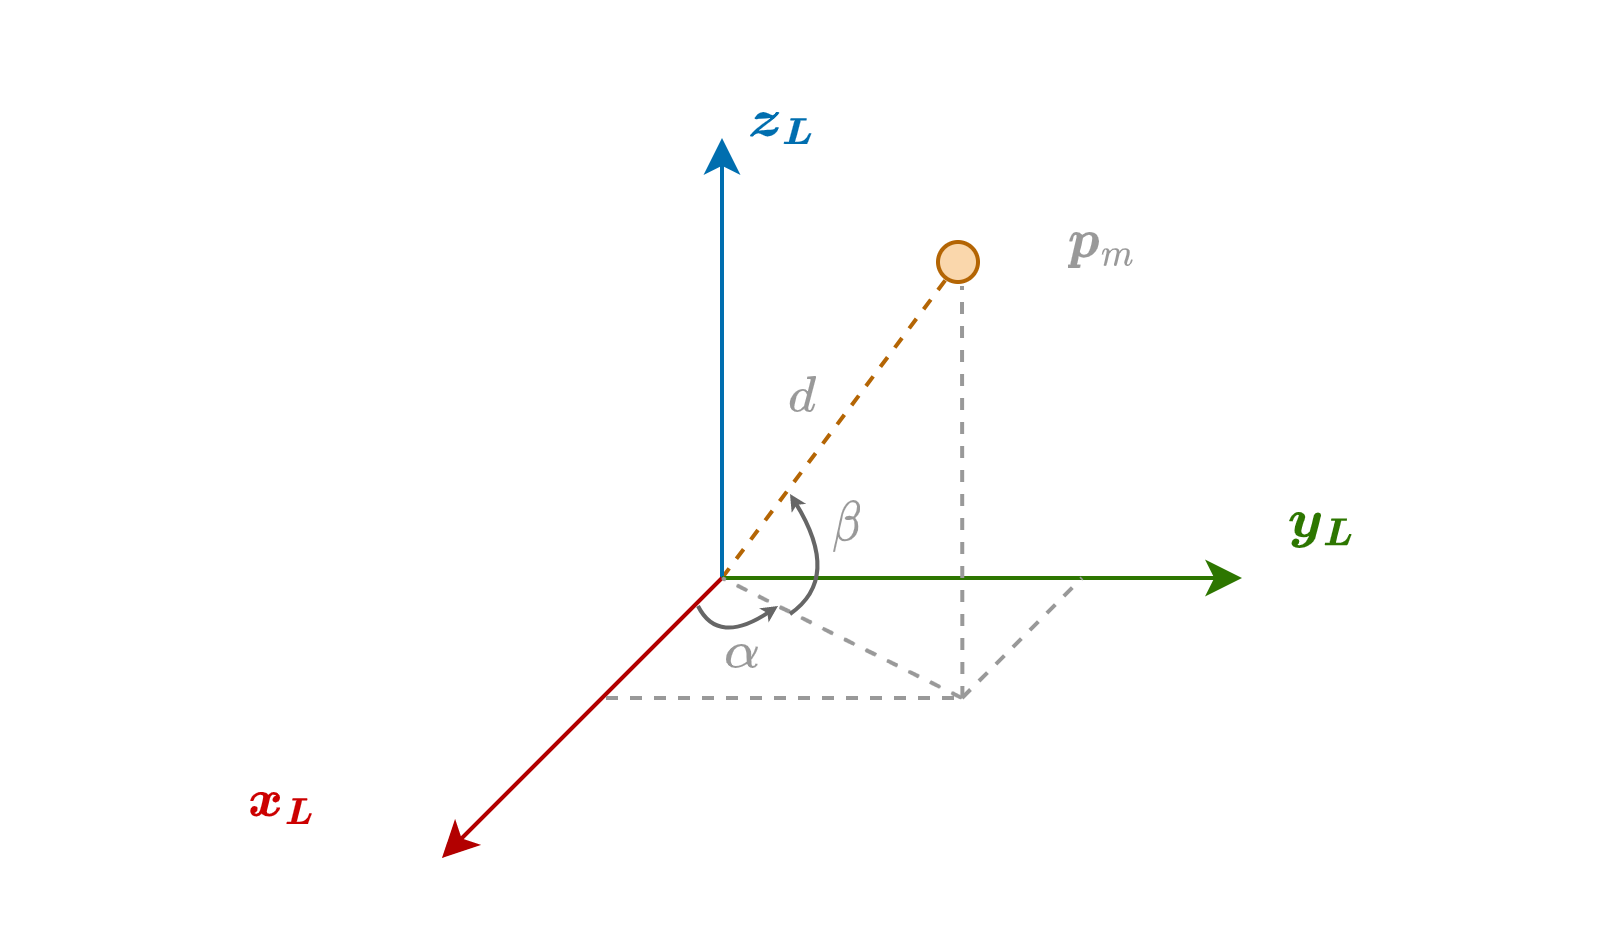
\includegraphics[width=0.48\linewidth]{img/lidar_model.png}
    %   \label{fig:lidar_model}
    % }
    % \subfigure[\normf{运动畸变}]{
    %   \centering
    %   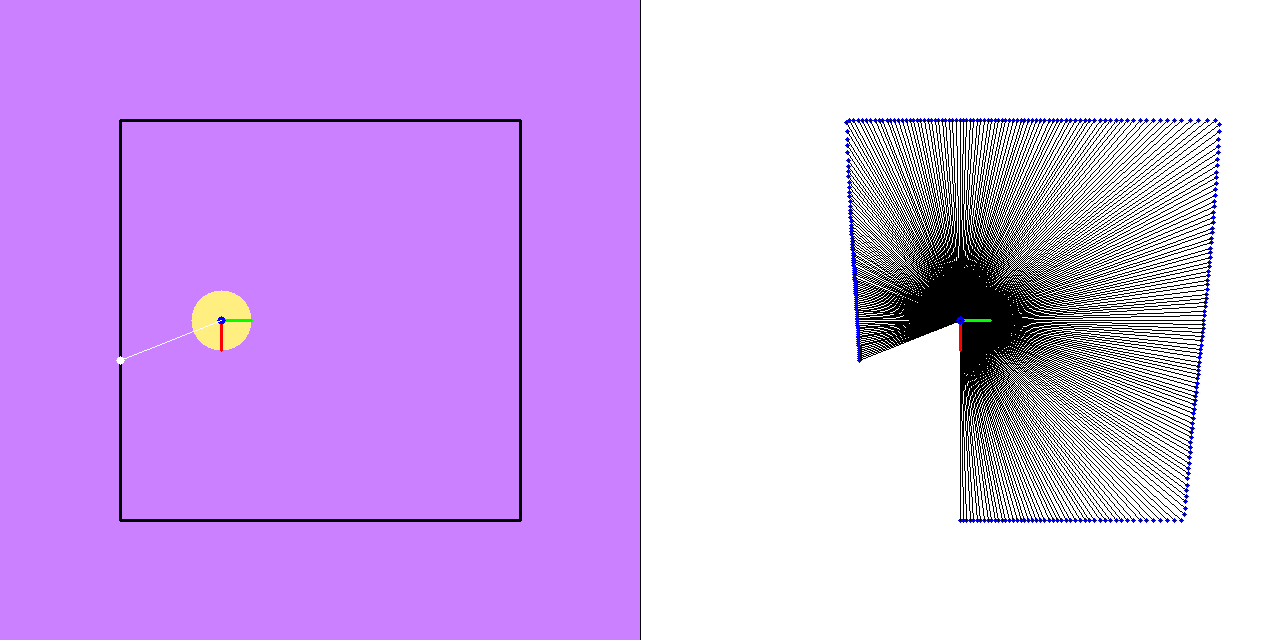
\includegraphics[width=0.48\linewidth]{img/lidar_motion_distort.png}
    %   \label{fig:lidar_motion_distort}
    % }
    \begin{subfigure}{0.48\textwidth}
      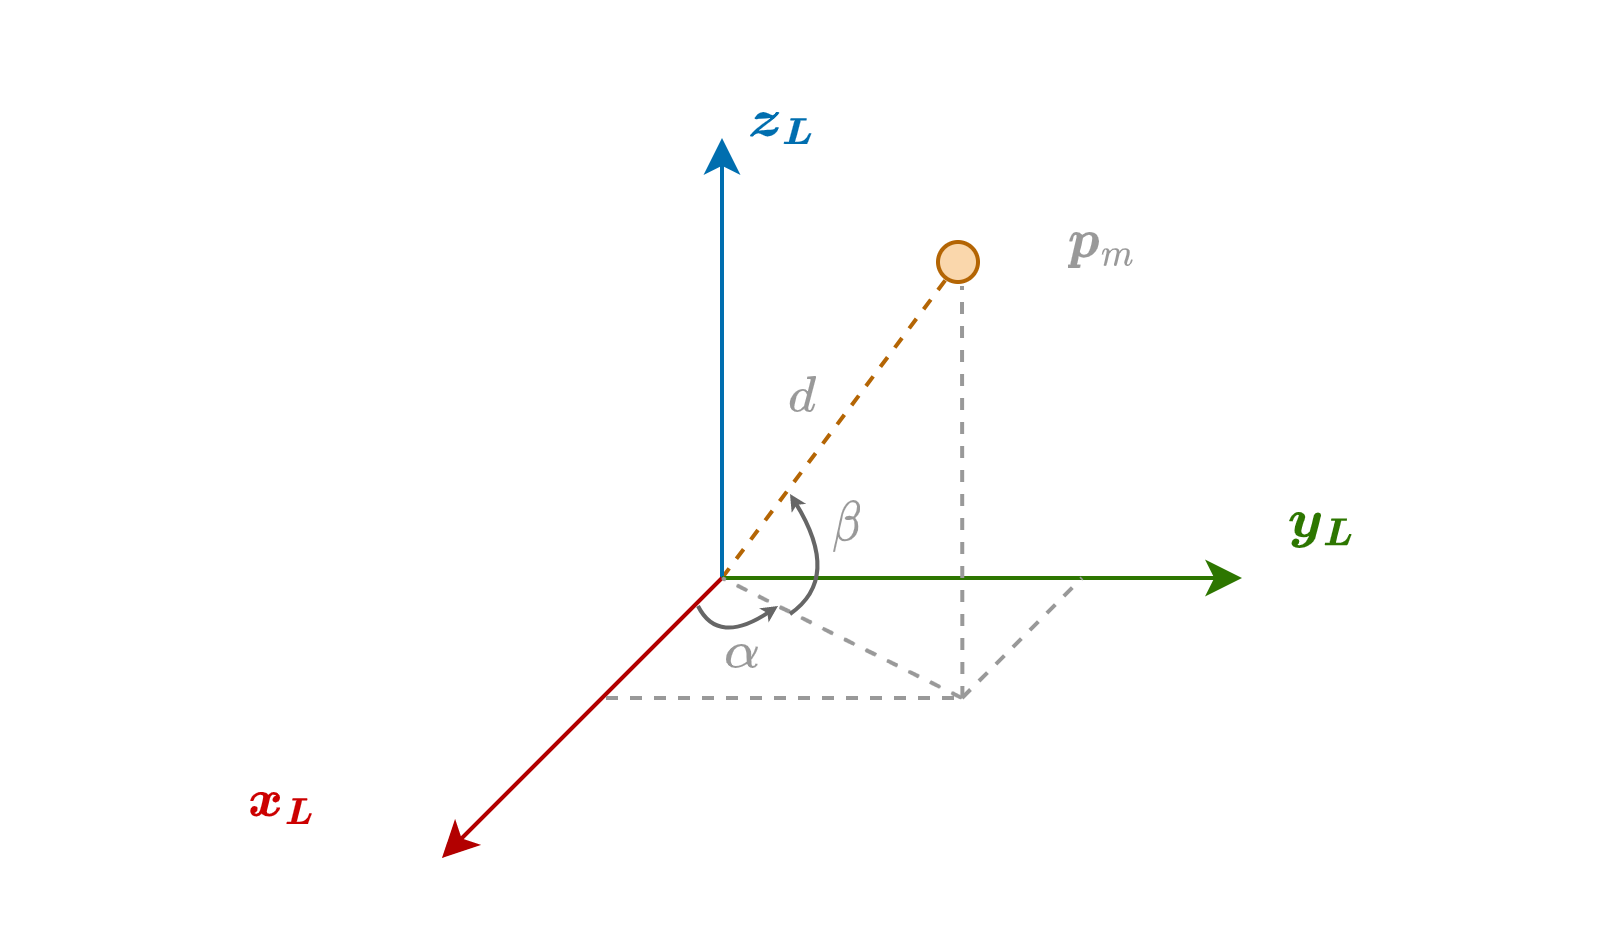
\includegraphics[width=\linewidth]{img/lidar_model.png}
      \caption{量测模型}
      \label{fig:lidar_model}
    \end{subfigure}
    \begin{subfigure}{0.48\textwidth}
      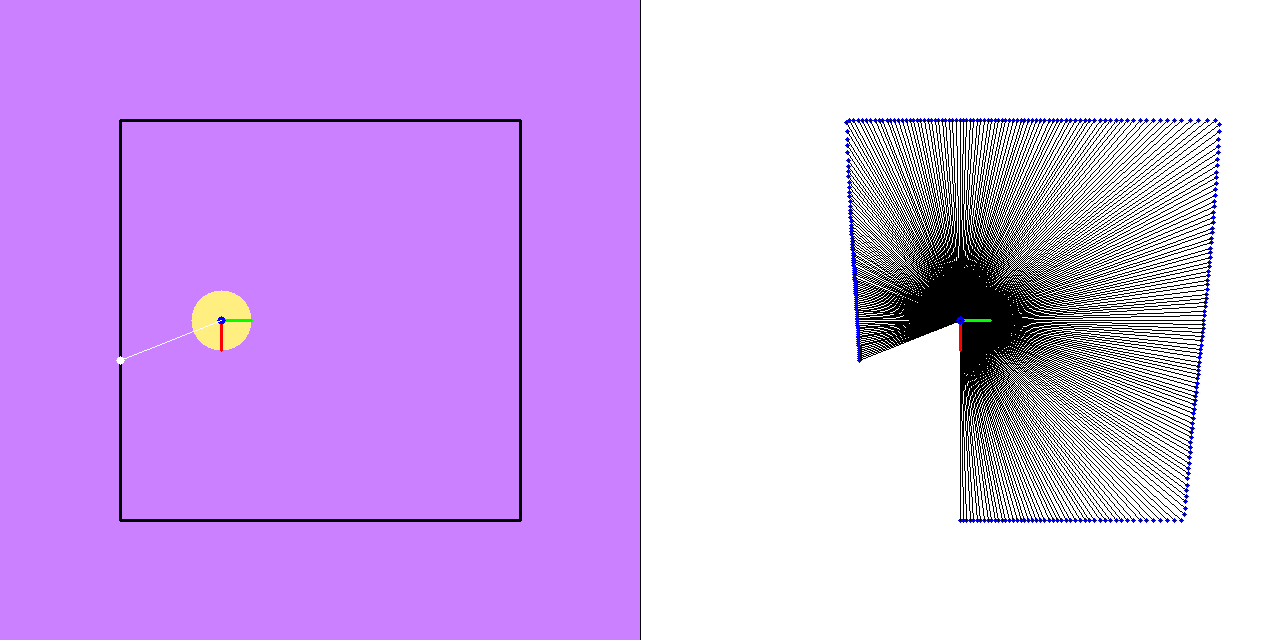
\includegraphics[width=\linewidth]{img/lidar_motion_distort.png}
      \caption{运动畸变}
      \label{fig:lidar_motion_distort}
    \end{subfigure}

    \caption{\normf{机械式激光雷达量测模型和运动畸变}}

    \label{fig:lidar}
  \end{figure}
}

机械式激光雷达存在待校准的内部参数,如每个激光发射器的高度角偏差、相对于理想L系的偏移量、测距偏差等,这些参数可以最终包含到一个相似变换(Similarity Transformation)里:
\begin{equation}
  \begin{pmatrix}
    {^{L}\boldsymbol{p}} \\1
  \end{pmatrix}={^{L}_{l_i}\boldsymbol{S}}\cdot
  \begin{pmatrix}
    {^{l_i}\widetilde{\boldsymbol{p}}} \\1
  \end{pmatrix}
  \quad\mathrm{s.t.}\quad
  {^{L}_{l_i}\boldsymbol{S}}=\begin{pmatrix}
    s_d\cdot{^{L}_{l_i}\boldsymbol{R}} & {^{L}\boldsymbol{t}_{l_i}} \\\boldsymbol{0}&1
  \end{pmatrix}\quad
  {^{l_i}\widetilde{\boldsymbol{p}}}=\begin{pmatrix}
    \widetilde{d}\times\cos\widetilde{\alpha}\times\cos\widetilde{\beta} \\
    \widetilde{d}\times\cos\widetilde{\alpha}\times\sin\widetilde{\beta} \\
    \widetilde{d}\times\sin\widetilde{\alpha}
  \end{pmatrix}
\end{equation}
其中:${^{l_i}\widetilde{\boldsymbol{p}}}$为根据目标点在第$i$个激光发射器坐标系下测得的距离$\widetilde{d}$、旋转角$\widetilde{\alpha}$和高度角$\widetilde{\beta}$计算得到的点坐标;${^{L}_{l_i}\boldsymbol{S}}$为第$i$个激光发射器坐标系$l_i$到理想雷达坐标系L的相似变换矩阵,相较于刚体变换多了一个关于测程$d$的尺度因子$s_d$。在实际应用中,由于这些偏差数值较小,影响有限且在可接受范围内,所以本文不考虑这些参数的标定,即认为机械式激光雷达为理想模型,其量测模型严格满足式\ref{equ:lidar_model}。

\subsection{\normf{Camera}}
相机可以将三维空间中的场景映射到二维像平面上,其和LiDAR一样,也是一种外部传感器。相机的成像模型较多,有针孔相机模型、等距相机模型、全向相机模型等,本文只讨论最简单的针孔相机模型。

针孔相机的成像模型所图\ref{fig:camera_model}所示。对于空间中的一物方点$\boldsymbol{p}_w$,其在像平面上的成像点为$\boldsymbol{p}_i$,则物方点$\boldsymbol{p}_w$、成像点$\boldsymbol{p}_i$和相机光心$\boldsymbol{O}$三点共线,即有:
\begin{equation}
  \label{equ:collinear}
  \frac{z_w}{f}=-\frac{y_w}{y_i}=-\frac{x_w}{x_i}\to
  \begin{cases}
    \begin{aligned}
      x_i & =-f\times\frac{x_w}{z_w} \\
      y_i & =-f\times\frac{y_w}{z_w}
    \end{aligned}
  \end{cases}
\end{equation}
其中$f$为相机的焦距,其值等于相机光心$\boldsymbol{O}$到像平面的垂直距离。对原始影像取倒像,可以将式\ref{equ:collinear}中的负号去除,该操作等价于将像平面挪到相机光心前面。像平面上点一般在像素坐标系下表达,坐标系原点$o$定义在图像的左上角,水平向右为$u$轴,垂直向下为$v$轴,构成平面$o$-$u$-$v$坐标系。

结合式\ref{equ:collinear},同时考虑像素大小和物理尺寸在横纵方向上的比例因子$s_x$、$s_y$(单位为:像素/$m$),可以得到:
\begin{equation}
  \label{equ:cam_pinhole}
  \begin{cases}
    \begin{aligned}
      u & =s_x\times f\times\frac{x_w}{z_w}+c_x \\
      v & =s_y\times f\times\frac{y_w}{z_w}+c_y
    \end{aligned}
  \end{cases}\to
  \begin{cases}
    \begin{aligned}
      u & =f_x\times x_n+c_x \\
      v & =f_y\times y_n+c_y
    \end{aligned}
  \end{cases}\to
  \begin{pmatrix}
    u \\v\\1
  \end{pmatrix}=\begin{pmatrix}
    f_x & 0   & c_x \\
    0   & f_y & c_y \\
    0   & 0   & 1
  \end{pmatrix}\begin{pmatrix}
    x_n \\y_n\\1
  \end{pmatrix}
\end{equation}
其中:$\boldsymbol{c}\left( c_x,c_y\right) $为相机光心在像平面上投影点(即像主点)的像素坐标;$\boldsymbol{p}_n\left(
  x_n,y_n\right) $为物方点$\boldsymbol{p}_w$在相机归一化平面\footnote{\normf{将相机坐标系下的点的Z坐标归1,即可将该点转换到相机归一化平面上。注意到,相机归一化平面上的点各维单位均为1。}}上的投影点;$\boldsymbol{p}\left(u,v \right) $为位于像平面上的成像点;$f_x$、$f_y$分别为横向和纵向上的缩放因子,简称为像素焦距,单位为像素。为方便后续表示,记$\boldsymbol{K}$为相机的内参矩阵,则将相机坐标系$C$下表达的物方点${^{C}\boldsymbol{p}_w}$投影到像平面上点$\boldsymbol{p}$的过程为:
\begin{equation}
  z_w\cdot\begin{pmatrix}
    \boldsymbol{p} \\1
  \end{pmatrix}=\boldsymbol{K}\cdot{^{C}\boldsymbol{p}_w}
  \quad\mathrm{s.t.}\quad
  \boldsymbol{K}=\begin{pmatrix}
    f_x & 0   & c_x \\
    0   & f_y & c_y \\
    0   & 0   & 1
  \end{pmatrix}
\end{equation}

相机在成像过程中,会受到透镜制造工艺和安装误差的影响,导致畸变效应的产生。对于针孔相机而言,一般将其建模为径向畸变和切向畸变\cite{高翔2017视觉},具体的公式如下:
\begin{equation}
  \label{equ:cam_pinhole_dist}
  \begin{cases}
    x_d=x_n(1+k_1r^2+k_2r^4+k_3r^6)+2p_1x_ny_n+p_2(r^2+2x_n^2) \\
    y_d=y_n(1+k_1r^2+k_2r^4+k_3r^6)+p_1(r^2+2y_n^2)+2p_2x_ny_n
  \end{cases}
\end{equation}
其中$r^2=x_n^2+y_n^2$为归一化平面上的点到该平面原点的距离平方,$\boldsymbol{p}_d\left( x_d,y_d	\right) $为加畸变后的点,其仍然位于归一化平面上。
%%%%%%%%%%%%%%%%%%%%%%%%%%%%%%%%%%%%%%%%%%%%%%%%%%%%%%%%%%%%%%%%%%%%%%%%%%%%%%%%%%%%%%%%%
\mlcomment{
  \begin{figure}[htbp]
    \centering

    \begin{subfigure}{0.48\textwidth}
      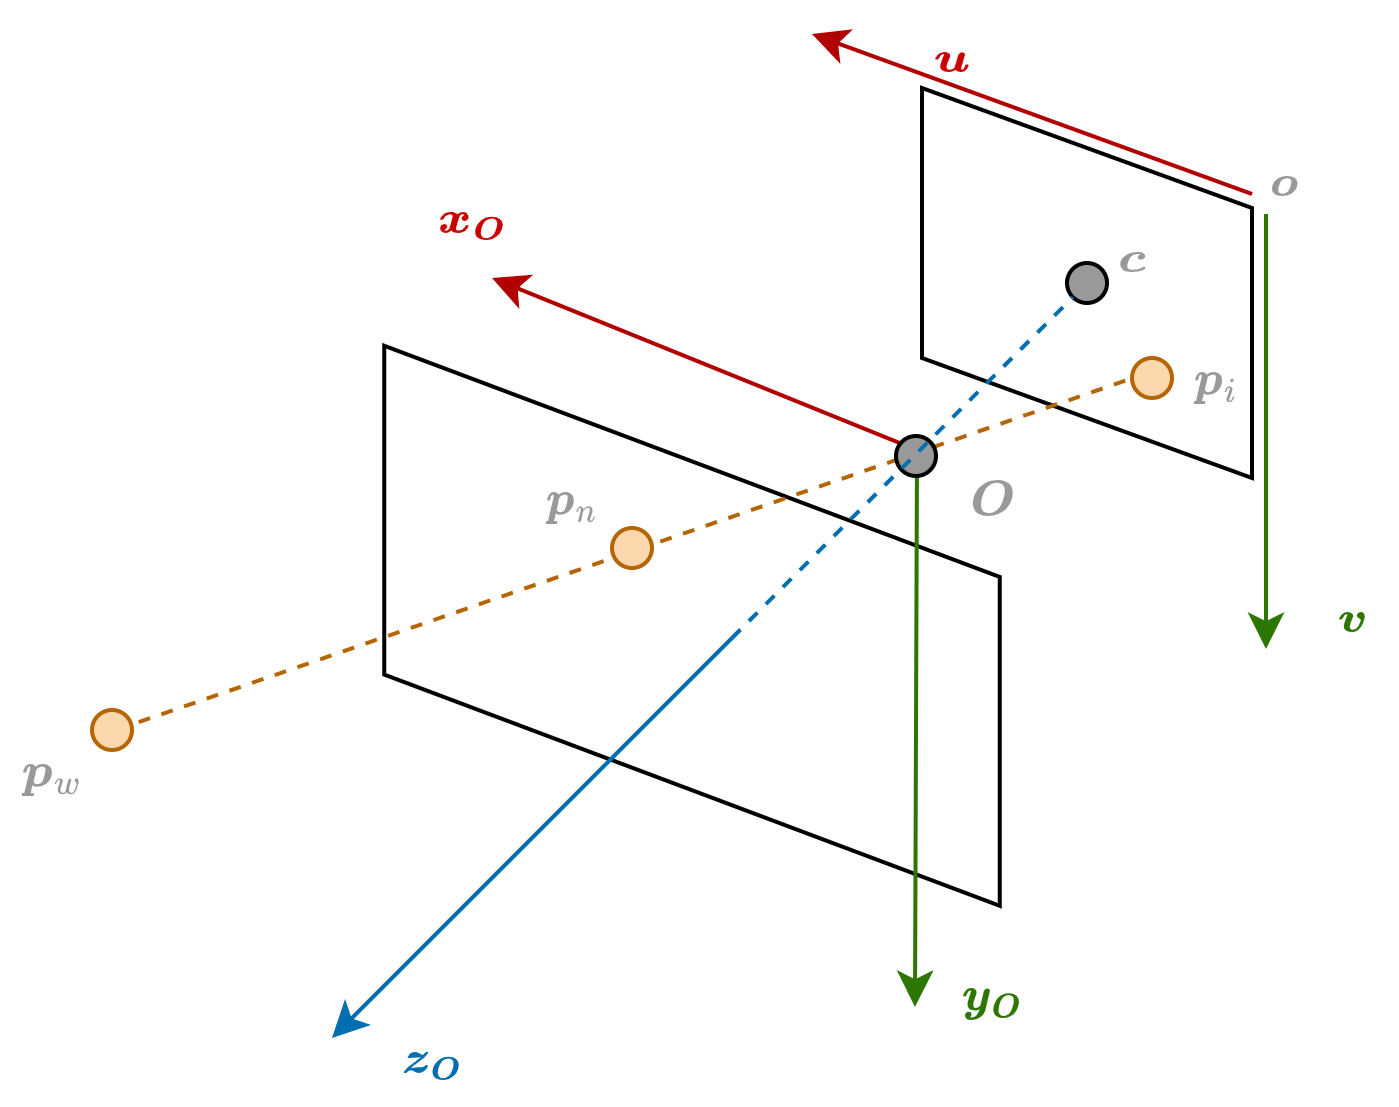
\includegraphics[width=\linewidth]{img/camera_model.png}
      \caption{量测模型}
      \label{fig:camera_model}
    \end{subfigure}
    \begin{subfigure}{0.48\textwidth}
      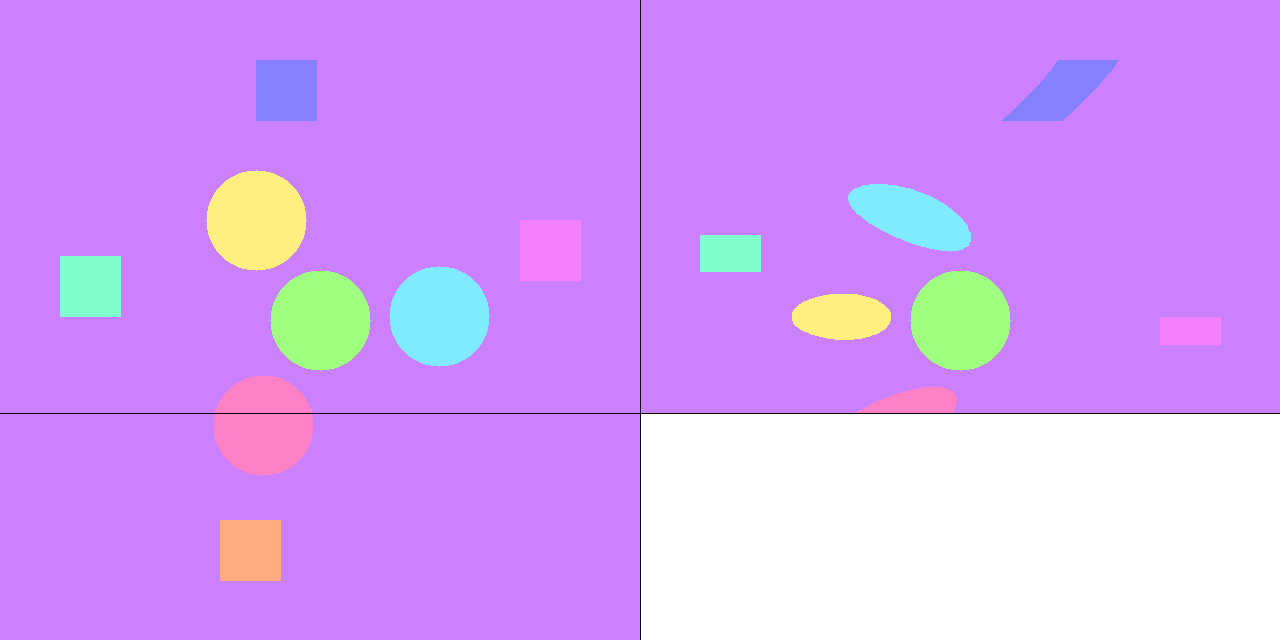
\includegraphics[width=\linewidth]{img/rs_camera_distort.png}
      \caption{果冻效应}
      \label{fig:rs_camera_distort}
    \end{subfigure}

    % \subcaptionbox{\normf{量测模型}}{
    %   \centering
    %   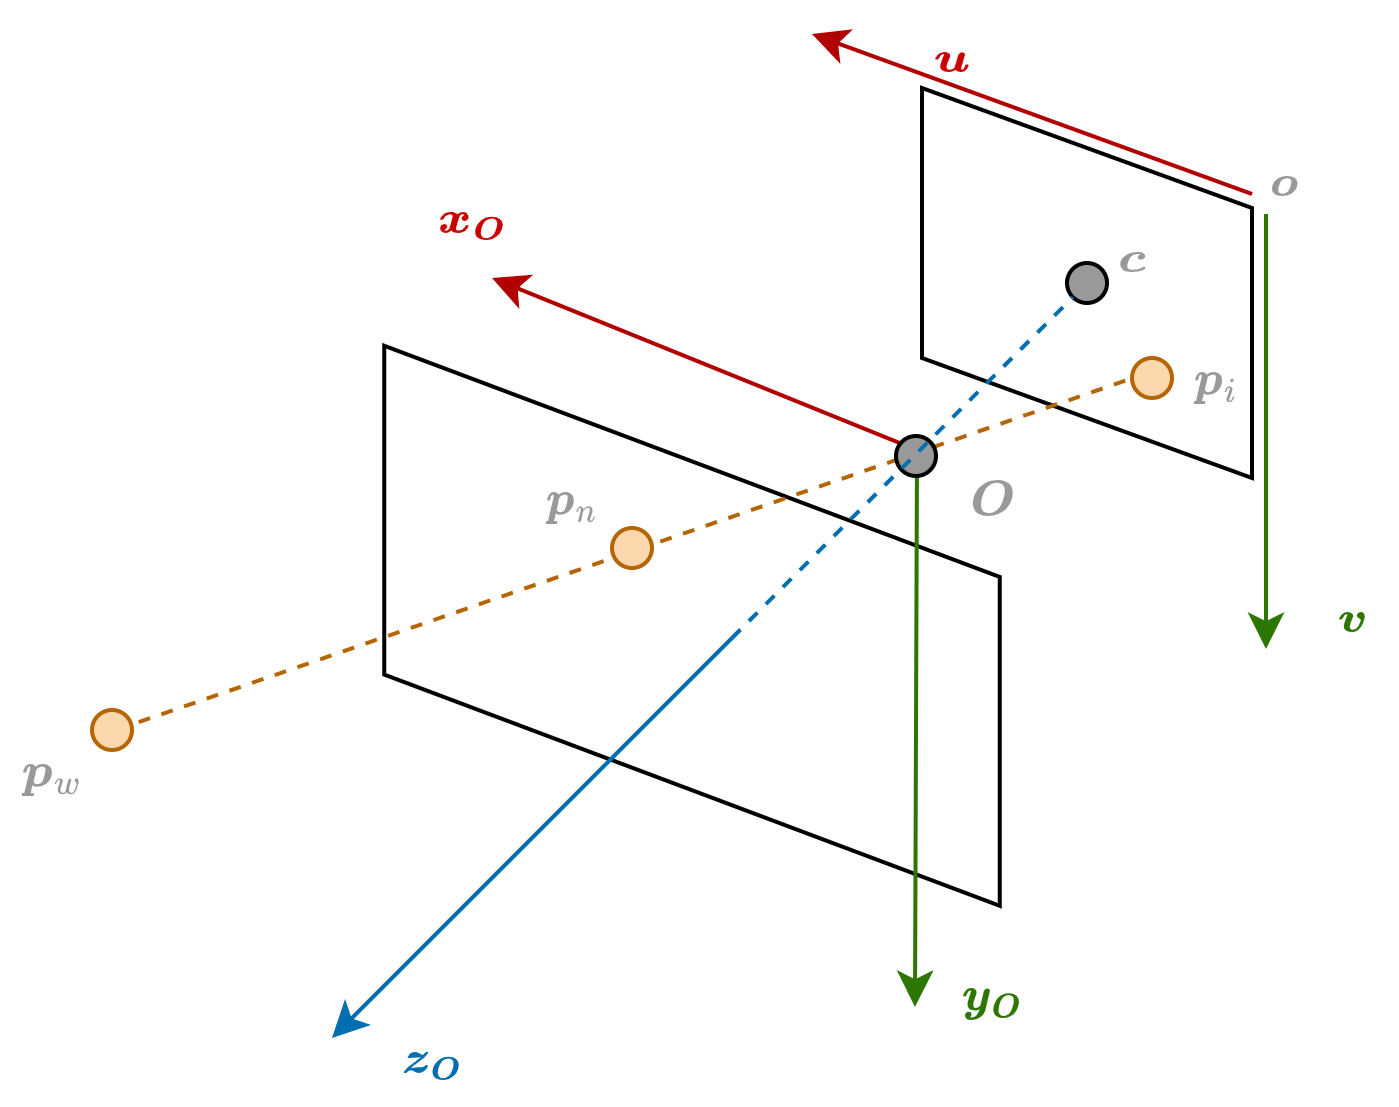
\includegraphics[width=0.48\linewidth]{img/camera_model.png}
    %   \label{fig:camera_model}
    % }
    % \subcaptionbox{\normf{果冻效应}}{
    %   \centering
    %   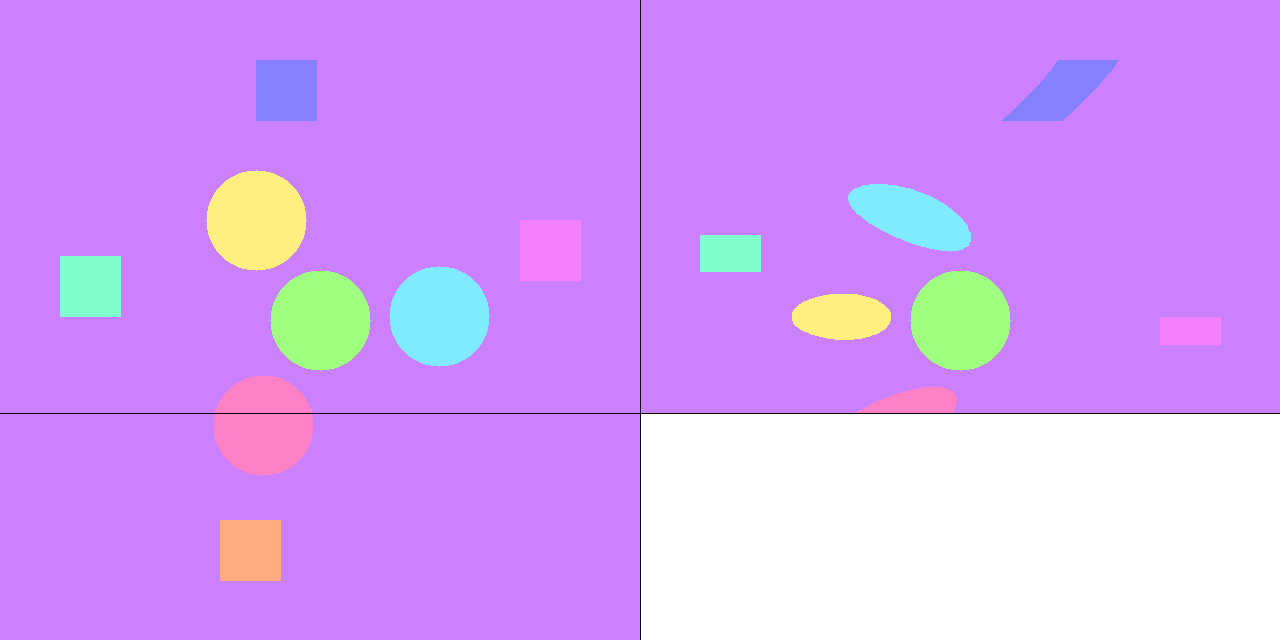
\includegraphics[width=0.48\linewidth]{img/rs_camera_distort.png}
    %   \label{fig:rs_camera_distort}
    % }


    \caption{\normf{卷帘式针孔相机量测模型和果冻效应}}

    \label{fig:camera}
  \end{figure}
}

对于针孔相机而言,可以根据曝光方式的不同,将其分为全局曝光相机(Global Shutter)和卷帘快门相机(Rolling Shutter)。全局曝光相机在同一时刻获取整幅影像上的像素强度;而卷帘快门相机则是通过行扫描的方式,在同一时刻获取单行的像素强度,因此同一幅影像上的不同行是异步采集的。相较于全局曝光相机,卷帘快门相机具有价格便宜、体积小、功耗低的优点,适合在移动平台上应用,比如手机、机器人、无人机等,因此本文标定使用的相机为卷帘快门相机\footnote{\normf{虽然本文研究的是卷帘快门相机,但是可以通过固定优化参数的方式,轻易地适配全局曝光相机。}}。

与机械激光雷达类似,卷帘快门相机的图像帧内是异步测量的,当场景中存在高速运动物体时,获取的影像存在畸变,称为果冻效应,如图\ref{fig:rs_camera_distort}所示。果冻效应会严重影响相关几何算法的精度,因此需要估计卷帘快门相机的读出时间(Readout Time)\footnote{\normf{即读出一幅图像帧总共所用的时间。由于读出单行时间是一致的,所以可以通过图像高度和行扫描时延计算得到。}}或行扫描时延(Line Delay)来去除畸变效应。


\subsection{\normf{IMU}}
惯性测量单元(Inertial Measurement Unit,IMU)由加速度计和陀螺仪组成。加速度计可以感知载体相对于惯性参考系的线加速度(即比力),陀螺仪则可以感知载体相对于惯性参考系的角速度。与激光雷达和相机不同,IMU是一种内部传感器,且其数据量更小,采样频率更高。根据实现原理的不同,加速度计和陀螺仪分为多种类别,本文使用的是MEMS惯性测量单元,其具有功率低、价格便宜的优点。

在对IMU进行建模时,本文主要考虑IMU的零偏(Bias)、比例因子(Scale Factor)和交轴耦合误差(Axis Misalignment),并顾及IMU的安装误差(IMU Misalignment)和量测噪声,即有:
\begin{equation}
  \label{equ:imu_model}
  \begin{cases}
    \begin{aligned}
      {^{G}}\boldsymbol{\omega}_m & =\boldsymbol{M}_\omega\cdot{^{G}_{I}\boldsymbol{R}}\cdot{^{I}}\boldsymbol{\omega}+\boldsymbol{b}_\omega+\boldsymbol{n}_\omega \\
      {^{A}}\boldsymbol{a}_m      & =\boldsymbol{M}_a\cdot{^{I}}\boldsymbol{a}+\boldsymbol{b}_a+\boldsymbol{n}_a
    \end{aligned}
  \end{cases}
\end{equation}
其中:${^{G}}\boldsymbol{\omega}_m$、${^{A}}\boldsymbol{a}_m$为陀螺仪和加速度计的原始输出;${^{I}}\boldsymbol{\omega}$、${^{I}}\boldsymbol{a}$为角速度和线加速度的理论值;$\boldsymbol{M}_{\omega\mid a}$矩阵包含了比例因子和交轴耦合误差(以加速度计为例,如图\ref{fig:imu_axis_mis}所示):
\begin{equation*}
  \boldsymbol{M}_\omega=\begin{pmatrix}
    S_{\omega 1} & M_{\omega 1} & M_{\omega 2} \\
    0            & S_{\omega 2} & M_{\omega 3} \\
    0            & 0            & S_{\omega 3}
  \end{pmatrix}\quad \boldsymbol{M}_a=\begin{pmatrix}
    S_{a 1} & M_{a 1} & M_{a 2} \\
    0       & S_{a 2} & M_{a 3} \\
    0       & 0       & S_{a 3}
  \end{pmatrix}
\end{equation*}
${^{G}_{I}\boldsymbol{R}}$为IMU的安装误差旋转矩阵(如图\ref{fig:imu_mis}所示)。本文以加速度计坐标系作为IMU坐标系,因此在处理角速度时,需要通过旋转矩阵${^{G}_{I}\boldsymbol{R}}$进行角速度向量的变换;$\boldsymbol{b}_\omega$、$\boldsymbol{b}_a$为陀螺仪和加速度计的零偏,本文建模为高斯随机游走;$\boldsymbol{n}_\omega$、$\boldsymbol{n}_a$分别为陀螺仪和加速度计的加性量测噪声,本文建模为零均值高斯白噪声。
%%%%%%%%%%%%%%%%%%%%%%%%%%%%%%%%%%%%%%%%%%%%%%%%%%%%%%%%%%%%%%%%%%%%%%%%%%%%%%%%%%%%%%%%%
\mlcomment{
  \begin{figure}[htbp]
    \centering

    \begin{subfigure}{0.48\textwidth}
      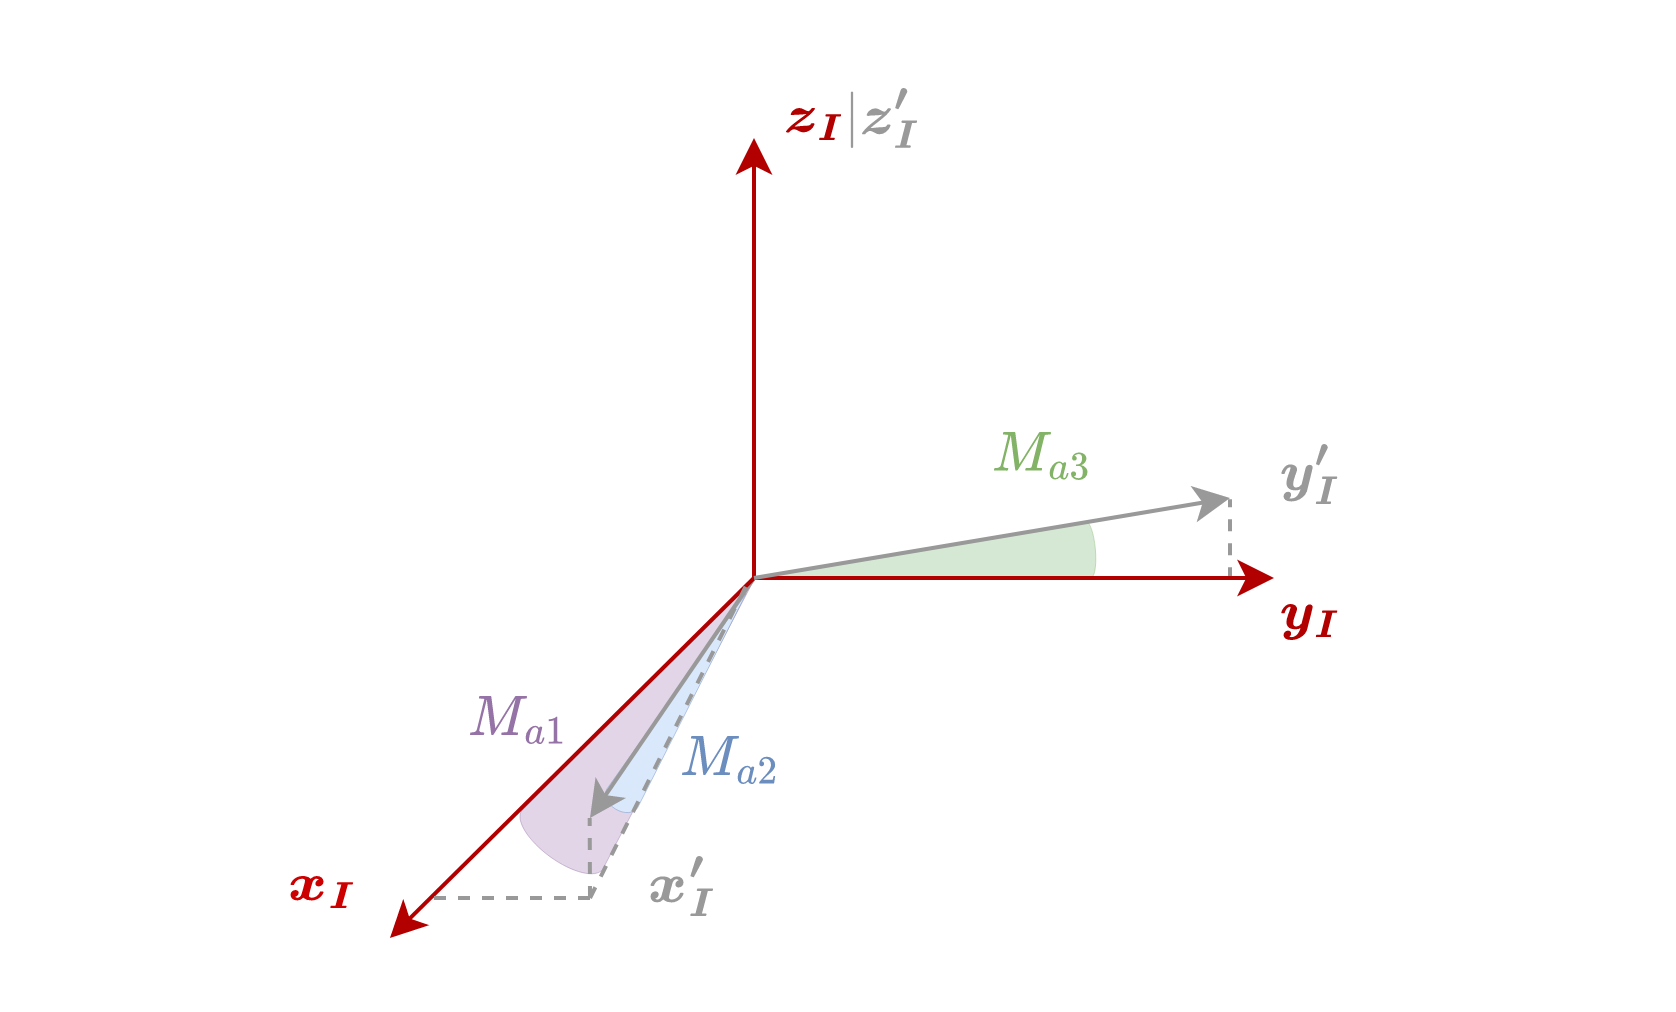
\includegraphics[width=\linewidth]{img/imu_axis_mis.png}
      \caption{交轴耦合误差}
      \label{fig:imu_axis_mis}
    \end{subfigure}
    \begin{subfigure}{0.48\textwidth}
      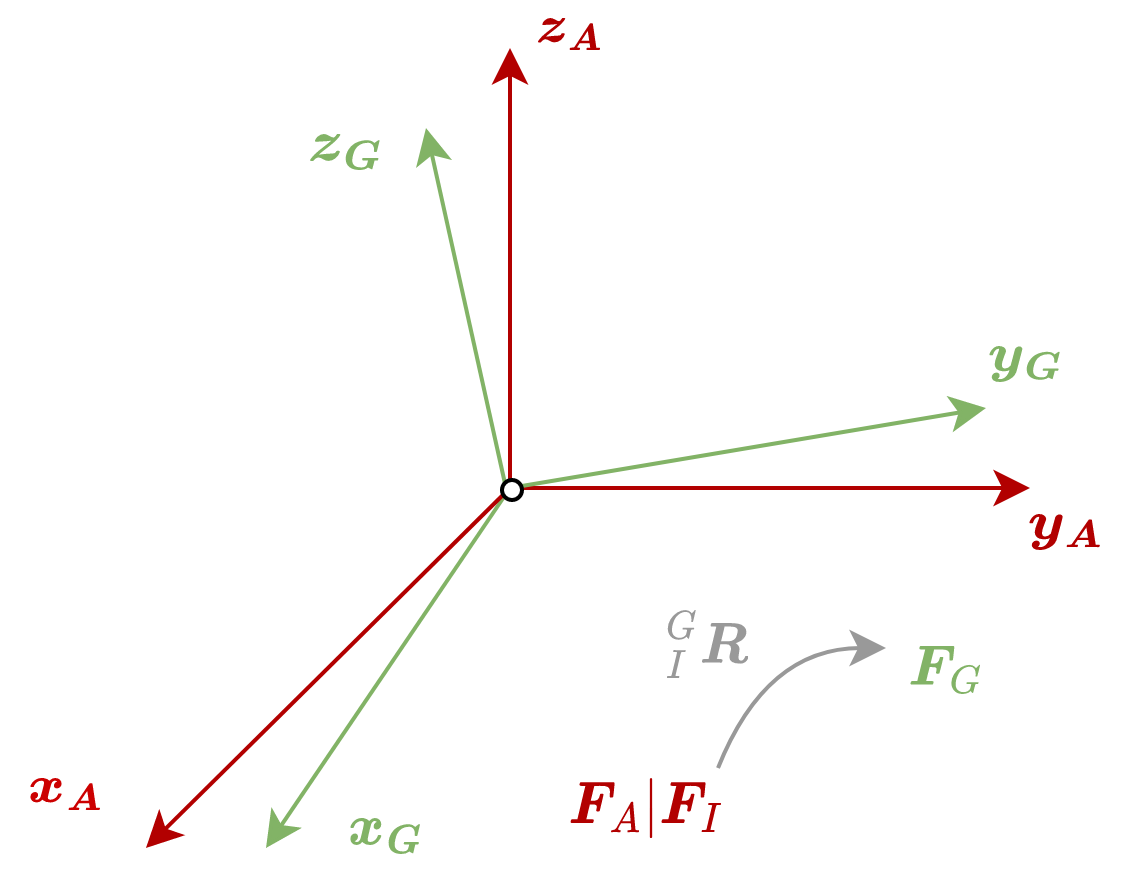
\includegraphics[width=\linewidth]{img/imu_mis.png}
      \caption{安装误差}
      \label{fig:imu_mis}
    \end{subfigure}
    % \subfigure[\normf{交轴耦合误差}]{
    %   \centering
    %   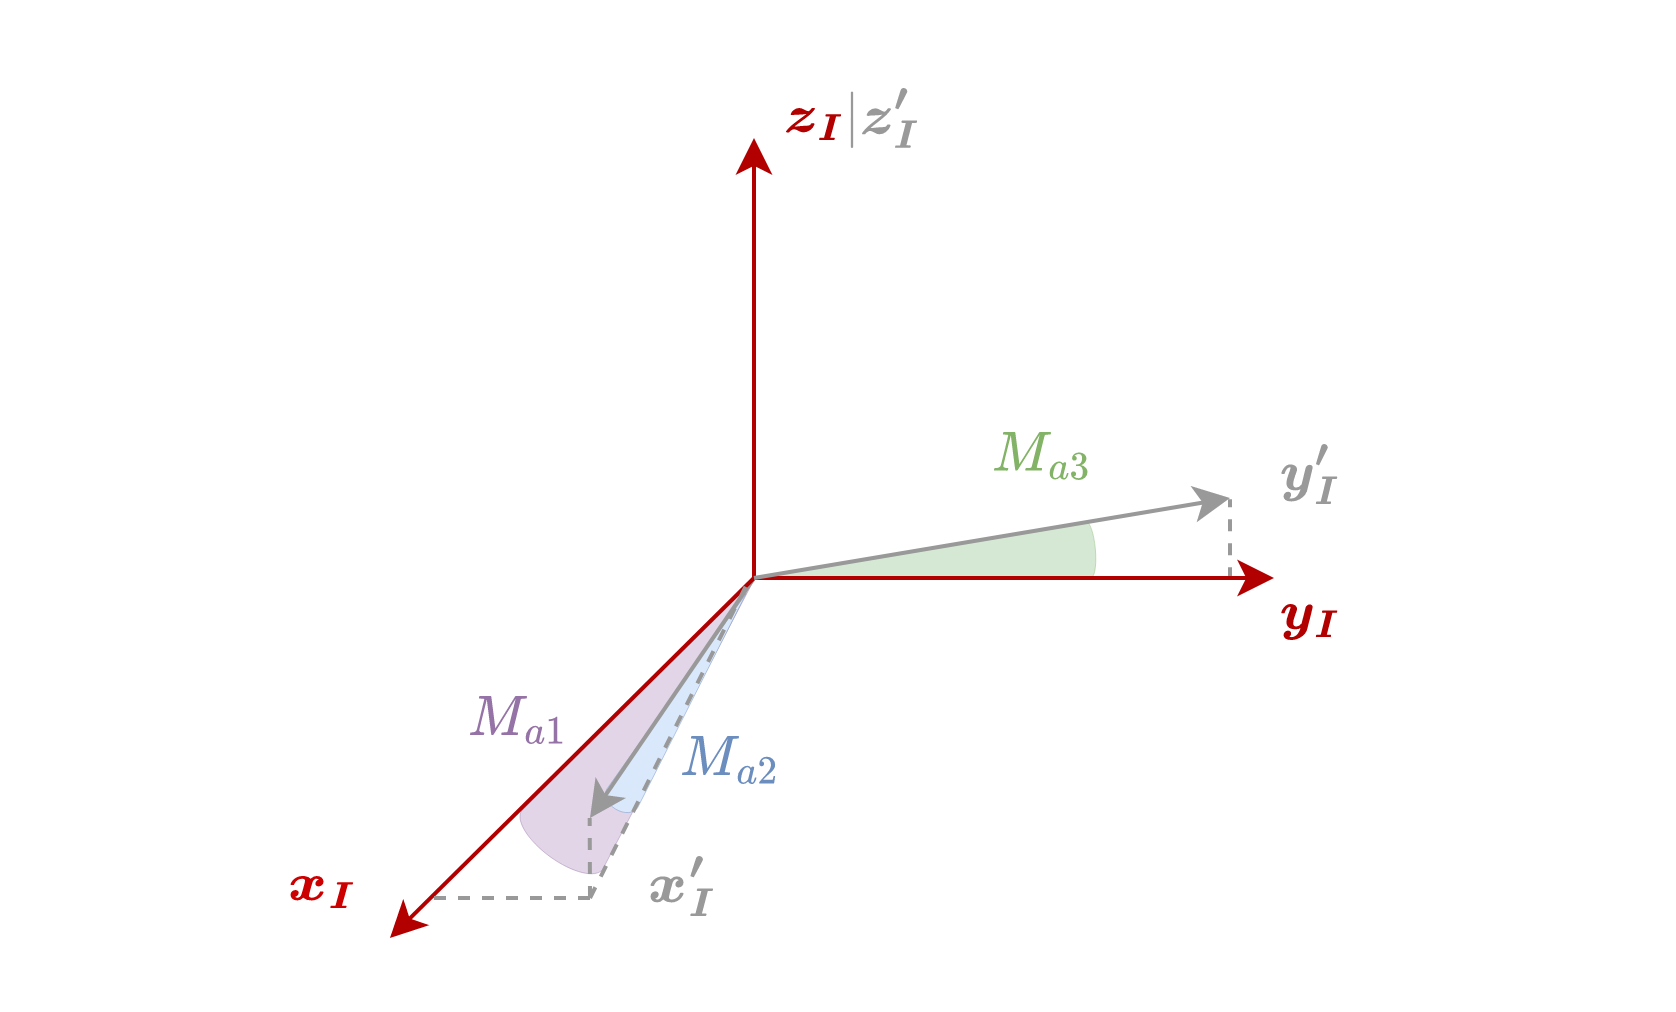
\includegraphics[width=0.48\linewidth]{img/imu_axis_mis.png}
    %   \label{fig:imu_axis_mis}
    % }
    % \subfigure[\normf{安装误差}]{
    %   \centering
    %   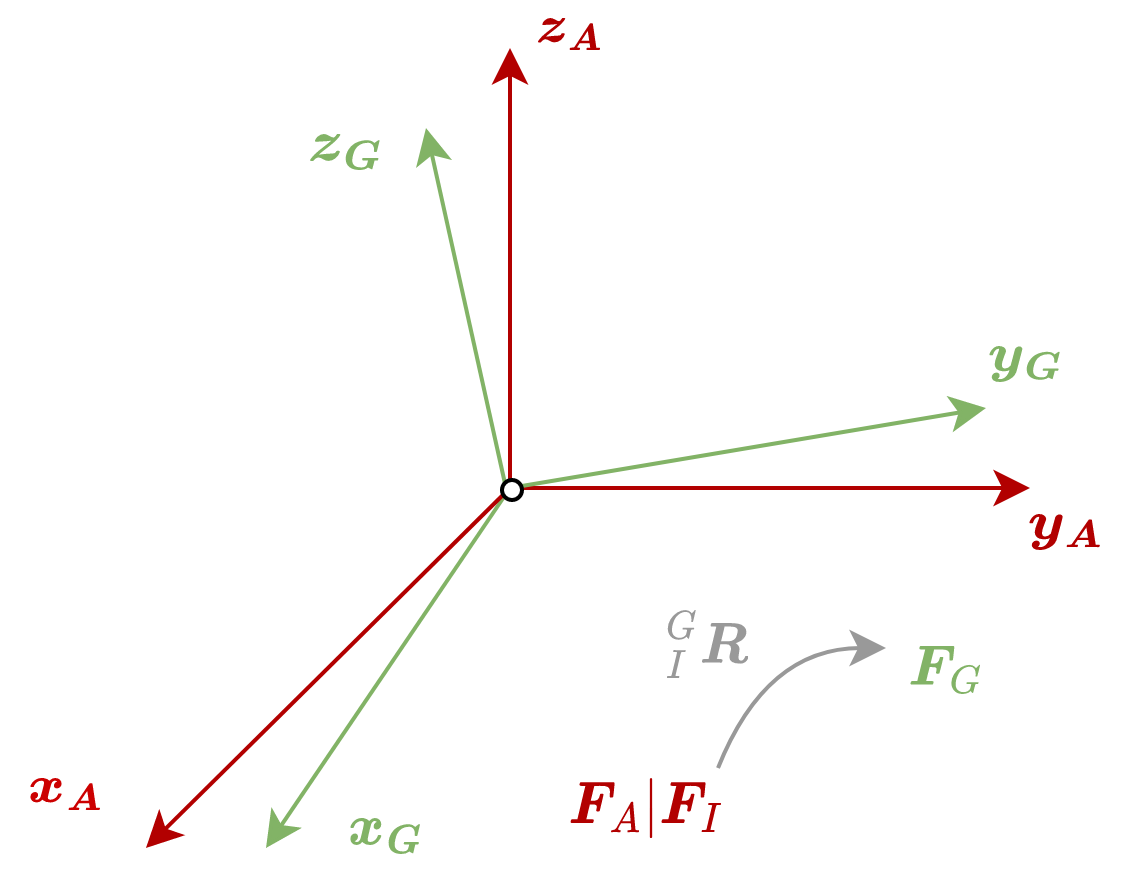
\includegraphics[width=0.48\linewidth]{img/imu_mis.png}
    %   \label{fig:imu_mis}
    % }

    \caption{\normf{IMU交轴耦合误差和安装误差}}

    \label{fig:imu}
  \end{figure}
}

\label{sensro_model_imu}

\subsection{\normf{待标参数}}
\label{suubsubsec:calib_param}
基于上文介绍的各传感器模型,下面给出本文标定框架中的待标参数:
\begin{enumerate}
  \item 外参

        外参描述不同传感器坐标系之间的变换关系,对于刚体变换而言,包含姿态量和平移量。本文待标外参有:
        \begin{itemize}
          \item $I$系与$L$系之间的外参:${^{I}_{L}}\boldsymbol{q}$、${^{I}}\boldsymbol{p}_{L}$;
          \item $I$系与$C$系之间的外参:${^{I}_{C}}\boldsymbol{q}$、${^{I}}\boldsymbol{p}_{C}$;
        \end{itemize}

  \item 内参

        内参描述传感器量测模型内部的映射关系,其具体形式取决于传感器的类型和量测模型建模方式。本文待标内参有:
        \begin{itemize}
          \item Camera内参:本文使用的相机模型为卷帘式针孔相机模型,在顾及相机的径向畸变和切向畸变下,内参有:像素焦距$f_x$、$f_y$,像主点像素坐标$c_x$、$c_y$,径向畸变参数$k_1$、$k_2$、$k_3$和切向畸变参数$p_1$、$p_2$。由于目前相机内参和畸变参数的标定算法已经成熟,故对于这些参数,本标定框架使用由粗到细(Coarse To Fine)的优化策略,基于给定初值进行精化;
          \item IMU内参:本文主要考虑IMU的安装误差旋转量${^{G}_{I}\boldsymbol{q}}$,加速度计和陀螺仪的比例因子和交轴耦合误差矩阵$\boldsymbol{M}_{a}$、$\boldsymbol{M}_{\omega}$,加速度计和陀螺仪的零偏$\boldsymbol{b}_a$、$\boldsymbol{b}_\omega$;
        \end{itemize}
        由于LiDAR内参偏差的影响在可接受范围内,故本文不予以考虑。
  \item 时参

        时参指与时间相关的参数。在进行粗略硬件同步的情况下,不同传感器时间系统之间会存在相对偏差,称为时延。时延的大小和传感器的设计、多传感器系统的架构、系统的运作环境\footnote{\normf{比如相机在不同亮度环境下采集图像,由于曝光时间的长短不同,会导致不同的时间偏差,这在本文的实测实验中也有体现(具体参考\ref{sec:exp_real_world}节)。}}等有关。另外对于卷帘快门相机,还存在读出时间。理论上读出时间属于和相机相关的参数,可以归为相机内参,但为了方便,本文将其划分为时参。基于此,本文待标时参有:
        \begin{itemize}
          \item IMU与LiDAR时参:$^{I}t_{L}$,IMU时间和LiDAR时间之间的转换关系为:$t_{I}=t_{L}+{^{I}t_{L}}$;
          \item IMU与Camera时参:$^{I}t_{C}$,IMU时间和Camera时间之间的转换关系为:$t_{I}=t_{C}+{^{I}t_{C}}$;
          \item
                卷帘快门相机读出时间:$t_{r}$,其定义方式与\cite{huai2022observability}一致,如图\ref{fig:gs_rs}所示。设图像帧的相机时间撮为图像首行的相机时间$t_C\left( 0\right)$,则对于第$v$行的像素,其相机时间为:
                \begin{equation}
                  \label{equ:readout_time}
                  t_C(v)=t_C\left( 0\right) +\frac{v}{h} \times t_r
                \end{equation}
                其中$h$为图像的高度。
        \end{itemize}

\end{enumerate}
\mlcomment{
  \begin{figure}[htbp]
    \centering
    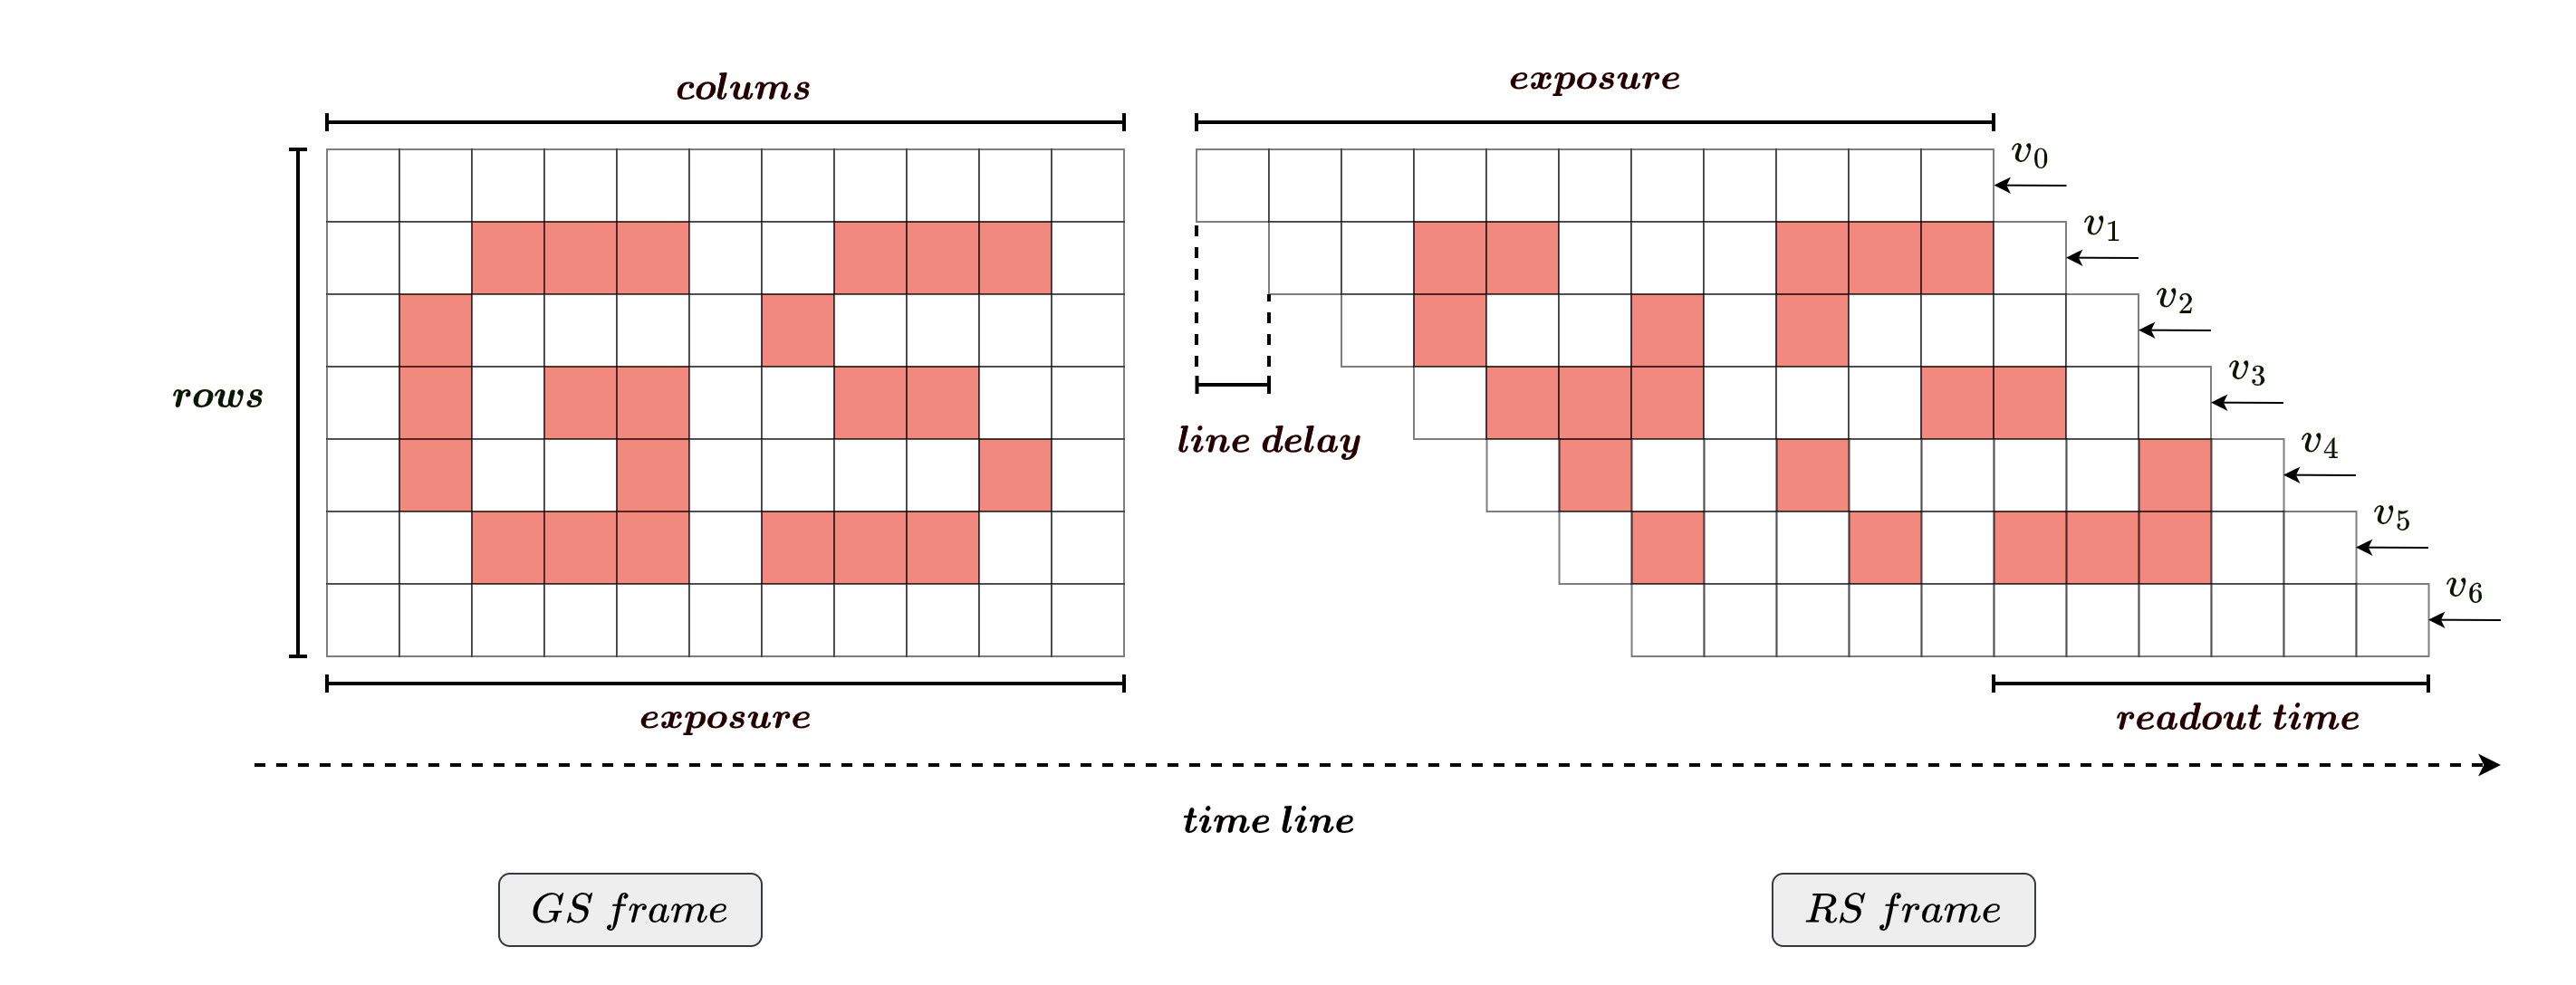
\includegraphics[width=0.95\linewidth]{img/gs_rs.png}

    \caption{\normf{GS相机全局曝光和RS相机行曝光}}

    \label{fig:gs_rs}
  \end{figure}
}

\section{\normf{连续时间理论}}
\subsection{\normf{离散时间和连续时间估计}}
本文所研究的标定算法是一种基于连续时间的无靶标标定方法,下面对离散时间理论和连续时间理论进行简要介绍。

真实世界中的传感器都是离散输出,如Camera和LiDAR输出帧率在10赫兹到30赫兹之间,IMU则可以达到上百赫兹。对于一个多传感器系统而言,在不考虑时延的情况下,直接处理不同传感器的同步离散输出来获取相关信息是一种简单有效的方法。但是当存在传感器异步测量时,需要进行时间同步,以消除异步测量带来的影响。一般而言,可以通过特制器件在硬件层面实现多传感器时间同步,但是这往往会增加系统的复杂度,成本也会更高。另一种时间同步方法是使用单一的中央处理单元(Central Processing Unit,CPU)记录不同传感器采集的数据帧的时间撮,在去除通信延迟后基于估计得到的常值时延进行时间同步。

对于后一种时间同步方法,目前存在两类方法:离散时间估计和连续时间估计。离散时间估计需要定制算法,以在估计过程中包含来自不同传感器的异步测量,且通常伴有相应的简化假设;而连续时间估计会先基于传感器的离散输出构建一个时间连续的函数,如B样条函数。当存在异步测量时,只需要对该函数进行采样,即可获取同步测量。

以机械激光雷达的运动畸变为例,由于同一点云帧中的不同点是异步测量,当LiDAR动态采集点云数据时,会导致畸变效应,因此需要进行时间同步。此时,离散时间估计方法一般会将运动简化为匀速运动或匀加速运动,而后基于已有的离散轨迹进行内插,如图\ref{fig:disc}所示。显然,当运动激烈时,这会引入较大的偏差。而连续时间估计方法会首先基于离散轨迹获取一个时间连续轨迹,如图\ref{fig:cont}所示,而后基于点云帧内各点的时间撮进行采样,并基于此消除运动畸变。
%%%%%%%%%%%%%%%%%%%%%%%%%%%%%%%%%%%%%%%%%%%%%%%%%%%%%%%%%%%%%%%%%%%%%%%%%%%%%%%%%%%%%%%%%
\mlcomment{
\begin{figure}[htbp]
  \centering

  \begin{subfigure}{0.48\textwidth}
    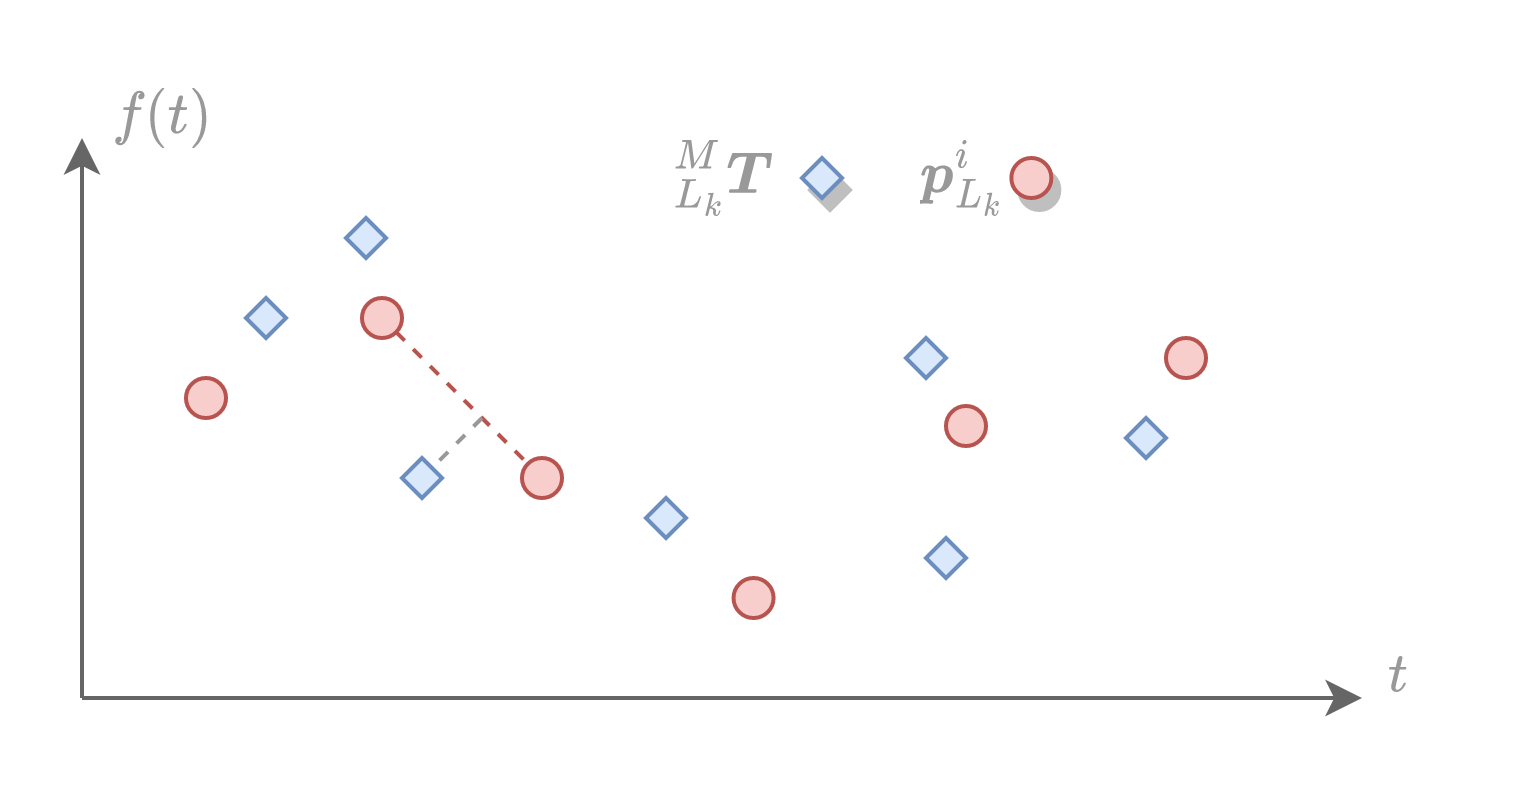
\includegraphics[width=\linewidth]{img/disc.png}
    \caption{离散时间估计}
    \label{fig:disc}
  \end{subfigure}
  \begin{subfigure}{0.48\textwidth}
    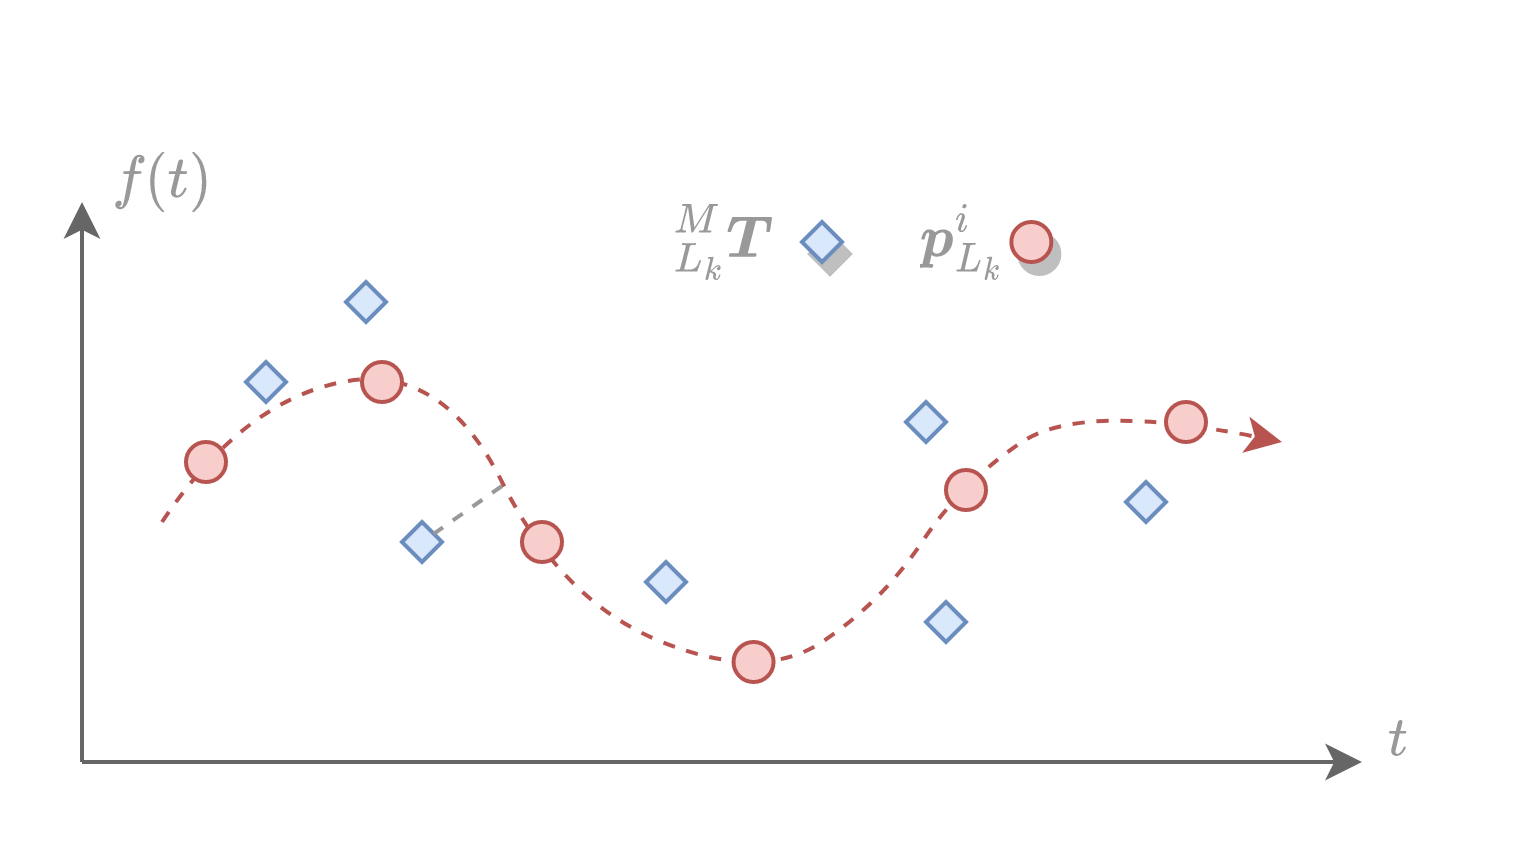
\includegraphics[width=\linewidth]{img/cont.png}
    \caption{连续时间估计}
    \label{fig:cont}
  \end{subfigure}
  % \subfigure[\normf{离散时间估计}]{
  %   \centering
  %   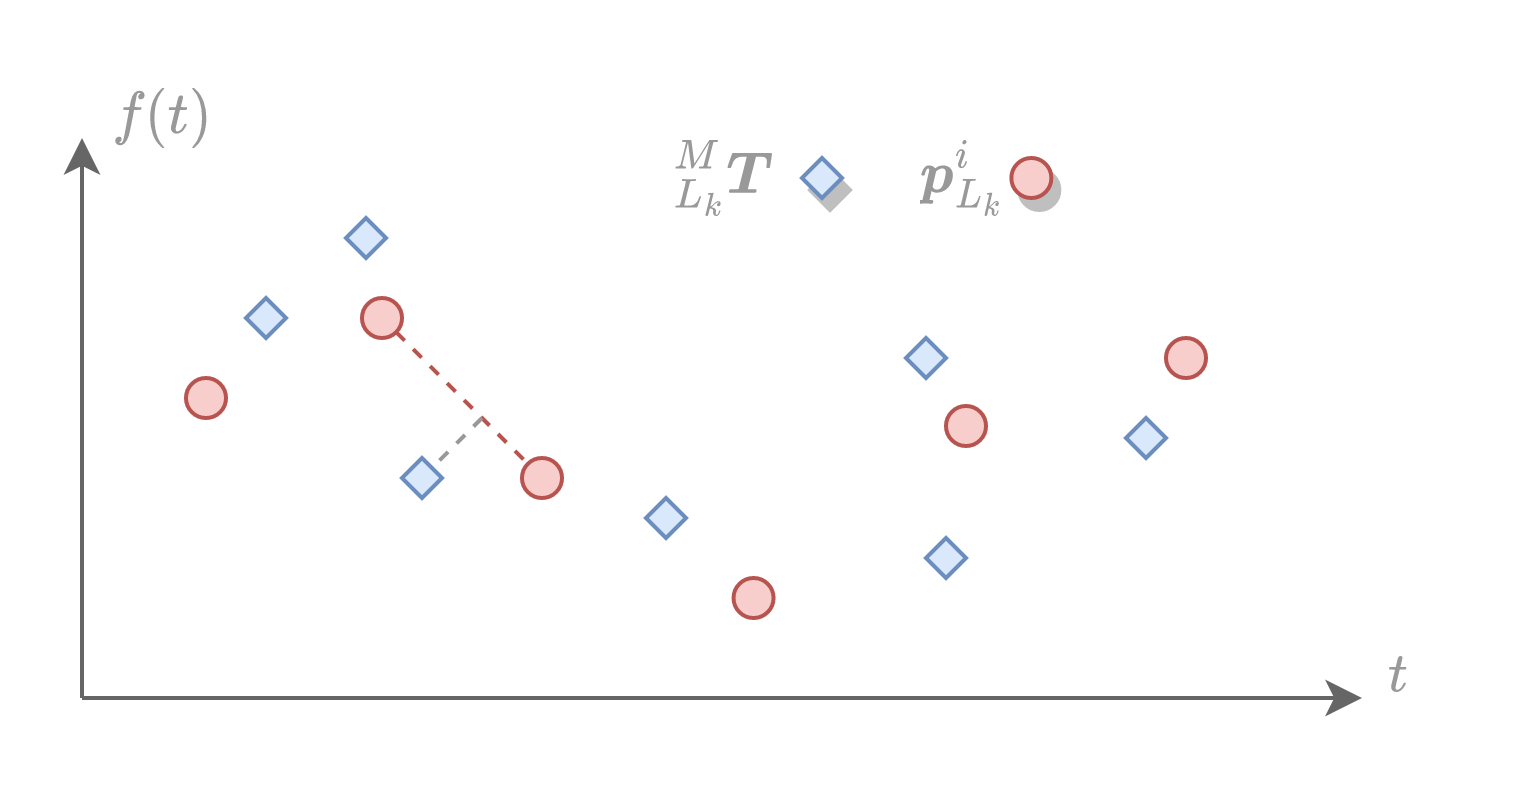
\includegraphics[width=0.48\linewidth]{img/disc.png}
  %   \label{fig:disc}
  % }
  % \subfigure[\normf{连续时间估计}]{
  %   \centering
  %   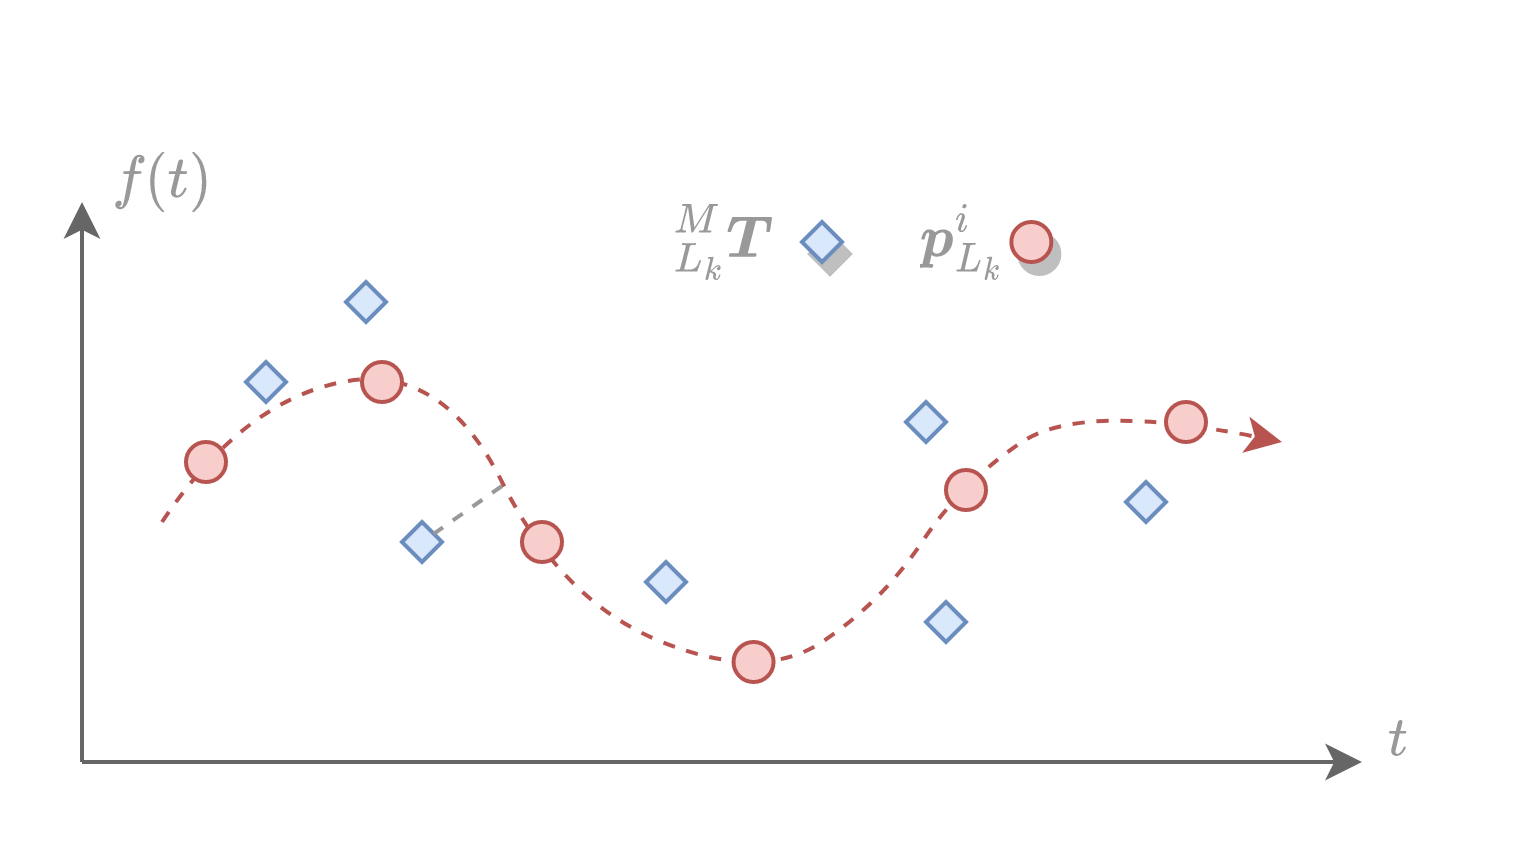
\includegraphics[width=0.48\linewidth]{img/cont.png}
  %   \label{fig:cont}
  % }

  \caption{\normf{基于离散时间估计和连续时间估计消除LiDAR帧运动畸变}}

  \label{fig:disc_cont}
\end{figure}
}

事实上,已有研究表明:当不存在传感器异步测量时,离散时间估计和连续时间估计结果是一致的;当存在传感器异步测量时,连续时间估计要优于离散时间估计\cite{cioffi2022continuous}。由于本文标定算法涉及时参的标定,因此采用连续时间估计。
\subsection{\normf{B样条位姿曲线}}
\label{subsubsec:pose_bspline}
上文提到,在使用连续时间估计时需要基于时间离散数据构建时间连续的函数,本文使用B样条曲线进行时间连续建模,下面对其进行介绍。

B样条曲线诞生于计算机图形学领域,目的是为了在不损失精度的条件下,用离散的控制点和相关控制参数(即阶次)表示一条连续的曲线。B样条曲线是贝塞尔曲线的一种扩展。贝塞尔曲线通过离散的控制点和参数来控制曲线,但局部控制点的变动会影响整条曲线的走向,即贝塞尔曲线局部是不可控的。而B样条曲线是局部可控的,局部控制点的变动只会影响局部曲线,不会对其他区域的曲线造成影响,具有较强的操控性,因此应用较为广泛。对于一条具有$n+1$个控制点的$d$次B样条曲线\footnote{\normf{B样条曲线的阶数(order)比次数(degree)多1,即$d$次B样条曲线的阶为$d+1$。}},其可表示为:
\begin{equation}
  \label{equ:b_spline_origin}
  \boldsymbol{B}_{n,d}(t)=\sum_{i=0}^{n}\boldsymbol{p}_i\cdot b_{i,d}(t)
\end{equation}
其中$b_{i,d}(t)$可以通过Cox-de Boor递归公式\cite{de1978practical}得到:
\begin{equation*}
  \begin{aligned}
    b_{i,0}(t) & =\begin{cases}
                    1\quad t_i\le t\le t_{i+1} \\
                    0\quad\dots
                  \end{cases}                                                                \\
    b_{i,d}(t) & =\frac{t-t_i}{t_{i+d}-t_i}b_{i,d-1}(t)+\frac{t_{i+d+1}-t}{t_{i+d+1}-t_{i+1}}b_{i+1,d-1}(t)
  \end{aligned}
\end{equation*}
当节点等距时,称B样条均匀。均匀B样条完全由阶次决定,且$t\in[t_i,t_{i+1}]$节点处的值只由$d+1$个控制点$\boldsymbol{p}_i,\boldsymbol{p}_{i+1},\cdots,\boldsymbol{p}_{i+d}$约束。阶次决定了B样条曲线的表达能力,阶次越高,表达能力越强。图\ref{fig:bspline}展示了控制点相同但阶次不同的均匀B样条曲线。
%%%%%%%%%%%%%%%%%%%%%%%%%%%%%%%%%%%%%%%%%%%%%%%%%%%%%%%%%%%%%%%%%%%%%%%%%%%%%%%%%%%%%%%%
\mlcomment{
  \begin{figure}[htbp]
    \centering
    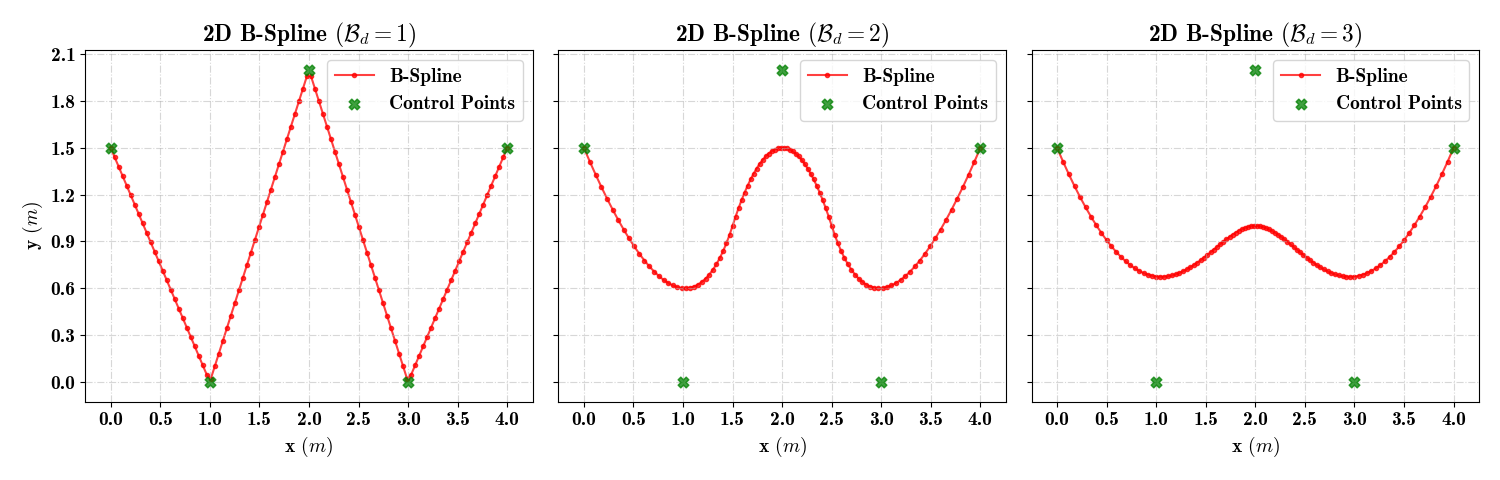
\includegraphics[width=0.95\linewidth]{img/bspline_2d.png}

    \caption{\normf{不同阶次的均匀B样条曲线比较}}

    \label{fig:bspline}
  \end{figure}
}

对于均匀B样条曲线而言,式\ref{equ:b_spline_origin}可以等价表示为更简洁的矩阵形式\cite{qin1998general}:
\begin{equation}
  \label{equ:matrix_bspline1}
  \boldsymbol{p}(t)=\sum_{j=0}^{d}\boldsymbol{u}^T\boldsymbol{M}^{(d+1)}_{(j)}\boldsymbol{p}_{i+j}
\end{equation}
其中:$\boldsymbol{u}^T=\begin{pmatrix}
    1 & u & \cdots & u^d
  \end{pmatrix}$,且$u=(t-t_i)/(t_{i+1}-t_i)$;$\boldsymbol{M}^{(d+1)}$是维度为$d+1$的方阵,$\boldsymbol{M}^{(d+1)}_{(j)}$表示其第$j$列。当$d$确定后,矩阵$\boldsymbol{M}^{(d+1)}$也就被唯一确定了。如在本文中,使用的是阶为4(即$d=3$)的B样条曲线表示轨迹,则:
\begin{equation*}
  \boldsymbol{M}^{(3+1)}=\frac{1}{6}\begin{pmatrix}
    1  & 4  & 1  & 0 \\
    -3 & 0  & 3  & 0 \\
    3  & -6 & 3  & 0 \\
    -1 & 3  & -3 & 1
  \end{pmatrix}\quad
  \boldsymbol{u}=\begin{pmatrix}
    1\\{u}\\{u}^2\\{u}^3
  \end{pmatrix}
\end{equation*}
进一步化简式\ref{equ:matrix_bspline1},可以得到:
\begin{equation}
  \label{equ:matrix_bspline2}
  \boldsymbol{p}(t)=\boldsymbol{p}_i+\sum_{j=1}^{d}\boldsymbol{u}^T\tilde{\boldsymbol{M}}^{(d+1)}_{(j)}(\boldsymbol{p}_{i+j}-\boldsymbol{p}_{i+j+1})
\end{equation}
当$d=3$时,上式中矩阵$\tilde{\boldsymbol{M}}^{(3+1)}$为:
\begin{equation*}
  \tilde{\boldsymbol{M}}^{(3+1)}=\frac{1}{6}\begin{pmatrix}
    6 & 5  & 1  & 0 \\
    0 & 3  & 3  & 0 \\
    0 & -3 & 3  & 0 \\
    0 & 1  & -2 & 1
  \end{pmatrix}
\end{equation*}

在使用均匀B样条曲线表示位姿轨迹时,可以采用姿态量和平移量分开的形式(即$\mathrm{SO}(3)+\mathbb{R}^3$),也可以采用二者耦合的形式(即SE(3))。后一种的精度更高,但其姿态量和平移量高度耦合,不利于控制平移曲线。而使用前一种解耦的方式分开表达位姿轨迹,更利于参数估计\cite{haarbach2018survey}。对于平移量,用式\ref{equ:matrix_bspline1}或式\ref{equ:matrix_bspline2}即可直接表示,但是对于姿态量而言,由于其在流行上其对数乘(本质上为加法)不封闭,需要作进一步处理\cite{高翔2017视觉}。具体而言,若用单位四元数表示姿态,则首先通过对数映射将旋转量从流行空间变换到代数空间,在数乘运算结束后通过指数映射回到流行空间,具体的推导可参考\cite{kim1995general}。这里直接给出结果:
\begin{equation}
  \boldsymbol{q}(t)=\boldsymbol{q}_i\circ \prod_{j=1}^{d}\exp\left( \boldsymbol{u}^T\tilde{\boldsymbol{M}}^{(d+1)}_{(j)}\log\left( \boldsymbol{q}_{i+j+1}^{-1}\circ \boldsymbol{q}_{i+j}\right) \right)
\end{equation}
其中$\circ$表示四元数乘法运算。

当使用均匀B样条曲线建立了时间连续的轨迹后,除了可以查询任意有效时刻的位姿外,还可以通过时间微分得到更高阶的轨迹信息,如速度、加速度、角速率等参量。比如,当使用IMU的离散位姿轨迹构建B样条曲线时,有:
\begin{equation}
  \label{equ:imu_bspline}
  \begin{cases}
    \begin{aligned}
      {^{I}\boldsymbol{a}(t)}      & ={^{I_0}_{I}\boldsymbol{R}^T(t)}\cdot({^{I_0}\ddot{\boldsymbol{p}}_I(t)}-{^{I_0}\boldsymbol{g}}) \\
      {^{I}\boldsymbol{\omega}(t)} & ={^{I_0}_{I}\boldsymbol{R}^T(t)}\cdot{^{I_0}_{I}\dot{\boldsymbol{R}}(t)}
    \end{aligned}
  \end{cases}
\end{equation}
其中:${^{I_0}\boldsymbol{g}}\in\mathbb{R}^3$表示首个IMU坐标系下的重力向量,在本文中将其模长设为常数$\vert \vert{^{I_0}\boldsymbol{g}}\vert\vert\approx 9.81m/s^2$,其自由度为2;${^{I_0}\ddot{\boldsymbol{p}}_I(t)}$表示$t$时刻的$I_t$系相对于$I_0$系的线加速度在$I_0$系下的表达;${^{I_0}_{I}\dot{\boldsymbol{R}}(t)}$表示$t$时刻的$I_t$系相对于$I_0$系的角速度在$I_0$系下的表达。

\section{\normf{因子图优化理论}}
\label{subsec:factor_graph}

从实现的角度出发,经典的优化估计问题可以分为两种:滤波方法和图优化方法。滤波方法一般基于马尔可夫性假设,计算效率高,但在处理非线性问题时会引入非线性误差。经典的滤波方法有卡尔漫滤波(Kalman Filter,KF)及其变种方法、粒子滤波(Particle Filter,PF)等。滤波方法的非线性误差可以通过迭代的方式多次线性化观测方程予以消除\cite{barfoot2017state},如迭代扩展卡尔漫滤波(Iterated Extended Kalman Filter,IEKF)。而图优化方法则在优化过程中多次线性化目标函数,更适合处理非线性问题,但计算效率稍低。图优化方法可以根据每次优化的规模,分为全局优化和局部优化\footnote{\normf{全局优化将所有待优化的参数一次性加入到优化图中进行优化估计,而局部优化则在优化过程中选择性地优化部分参数,其余参数被固定,不进行优化。SLAM领域经典的滑窗优化即为一种局部优化。}},后者只能保证局部最优,但是计算效率高。由于多传感器标定是一个高度非线性的问题,因此本文使用图优化方法进行参数估计。下面对图优化理论进行简单介绍。

对一个优化估计问题,可以通过分解的方式对其进行建模,如使用贝叶斯网络(Bayesian
Networks)、马尔可夫随机域(Markov Random Fields)、因子图(Factor Graphs)等。与贝叶斯网络使用概率密度建模不同,因子图通过因式分解的方式建模优化问题,因此可以将任何因子函数纳入到优化图中\cite{dellaert2017factor},如下所示:
\begin{equation}
  \label{equ:factor_graphs}
  p(x_1,x_2,\cdots,x_n)\propto\prod f_1(x_i,x_j,\cdots)\times f_2(x_j,x_k,\cdots)\times\cdots\times f_m(x_k,x_l,\cdots)
\end{equation}
其中$f_m$为因子函数,简称为因子;$x_n$为待优化变量,称为节点。优化的目标是使得式\ref{equ:factor_graphs}中的概率密度$p$最大,一般通过最大后验估计(Maximum A Posteriori,MAP)实现。因子图可以非常方便的表示因子化的过程,如对于式\ref{equ:factor_graphs}而言,其可表示为图\ref{fig:factor_graphs}所示的因子图。
%%%%%%%%%%%%%%%%%%%%%%%%%%%%%%%%%%%%%%%%%%%%%%%%%%%%%%%%%%%%%%%%%%%%%%%%%%%%%%%%%%%%%%%%%
\mlcomment{
  \begin{figure}[htbp]
    \centering
    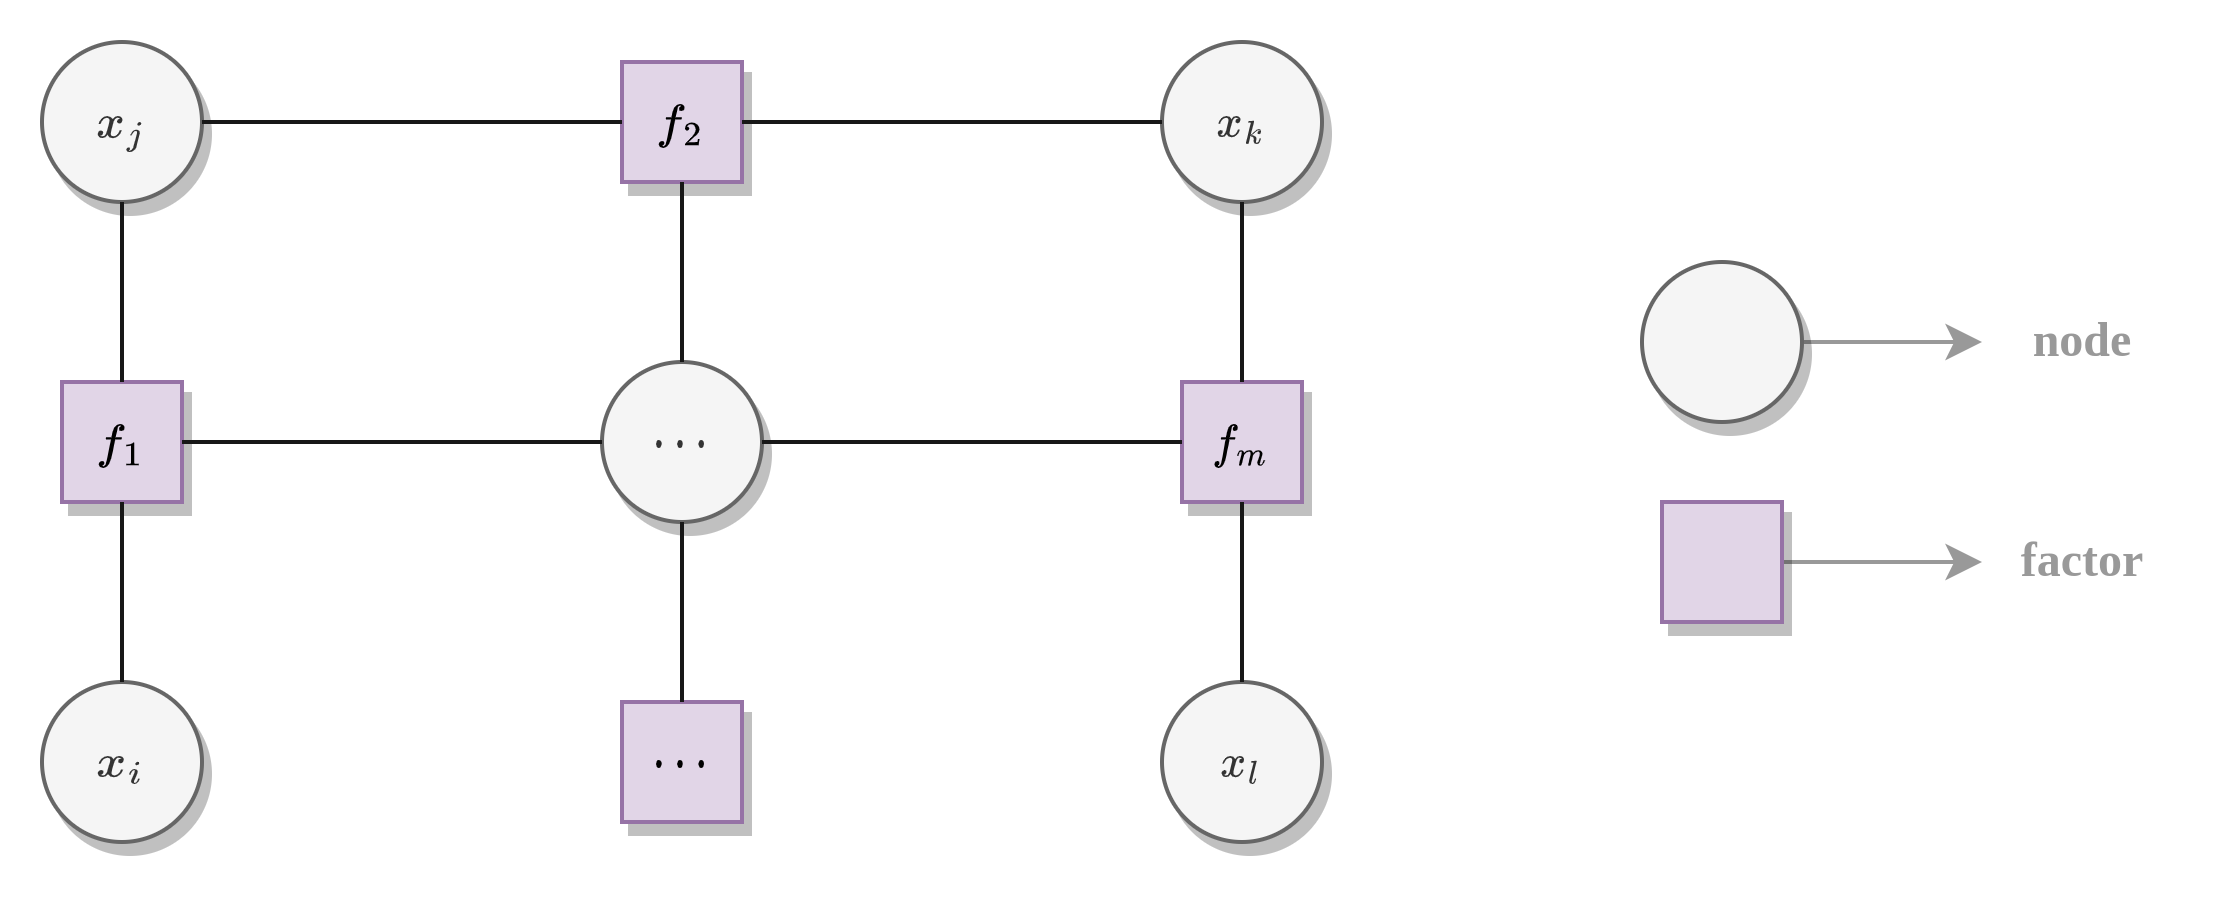
\includegraphics[width=0.5\linewidth]{img/factor_exam.png}
    \caption{\normf{因子图优化的图表示}}
    \label{fig:factor_graphs}
  \end{figure}
}

对于图优化问题的求解,目前已有许多优秀的开源框架,如Ceres\cite{agarwal2012ceres}、$g^2o$\cite{grisetti2011g2o}、GTSAM\cite{dellaert2012factor}、SE-
Sync\cite{rosen2020certifiably}。本文在处理图优化问题时使用Ceres图优化框架, 因为相较于其他开源框架,Ceres在易用性、可扩展性、安全性以及计算效率等方面都比较突出\cite{juric2021comparison}。

% Chapter 3

\chapter{引用与链接}

\section{脚注}
注释是对论文中特定名词或新名词的注解。注释可用页末注或篇末注的一种。选择页末注的应在注释与正文之间加细线分隔,线宽度为 1 点,线的长度不应超过纸张的三分之一宽度。同一页类列出多个注释的,应根据注释的先后顺序编排序号。字体为宋体5号,注释序号以“\circled{1}、\circled{2}”等数字形式标示在被注释词条的右上角。页末或篇末注释条目的序号应按照“\circled{1}、\circled{2}”等数字形式与被注释词条保持一致,脚注序号每面更新。示例:这里有个注释\footnote{我是解释注释的}。 

\section{引用文中小节}\label{sec:ref}
如引用小节~\ref{sec:ref}

\section{引用参考文献}
这是一个参考文献引用的范例:“\cite{江泽民1989能源发展趋势及主要节能措施}提出……”。还可以引用多个文献:“\cite{kuhn2004man,江泽民2008新时期我国信息技术产业的发展,江泽民1989能源发展趋势及主要节能措施}提出……”。不同的引用方法:“\citet{江泽民1989能源发展趋势及主要节能措施}”“\citep{江泽民2008新时期我国信息技术产业的发展}”更多引用命令请参阅 natbib 文档或 biblatex 文档。\nocite{*}

文献引用需要配合 BibTeX 使用,很多工具可以直接生成 BibTeX 文件(如 EndNote、NoteExpress、百度学术、谷歌学术等),此处不作介绍。

\section{链接相关}
模板使用了 hyperref 包处理相关链接,使用 \verb|\href| 可以生成超链接,默认不显示链接颜色。如果需要输出网址,可以使用 \verb|\url| 命令,示例:\url{https://github.com}。
\chapter{\normf{实验验证}}
为了验证本文所提出的基于连续时间的LiDAR/Camera/IMU时空标定方法的可行性,我们基于GAZEBO虚拟仿真平台进行了仿真实验。结果证明,在运动充分激励条件下,整个标定系统是可观的(具体的系统可观性分析见\ref{appendix:observability}节的系统可观性实验),能够实现相关参数的正确估计。随后,我们基于自主搭建的实验平台进行了实测实验,对所提出的算法进行综合的测试和评估。最后,我们对不同运动形式下的系统可观性进行分析和实验验证。下面对三个实验进行说明和相应分析讨论。

\section{\normf{仿真实验}}
%%%%%%%%%%%%%%%%%%%%%%%%%%%%%%%%%%%%%%%%%%%%%%%%%%%%%%%%%%%%%%%%%%%%%%%%%%%%%%%%%%%%%%%%%
\mlcomment{
  \begin{figure}[htbp]
    \centering

    \subfigure[\normf{斜视图}]{
      \centering
      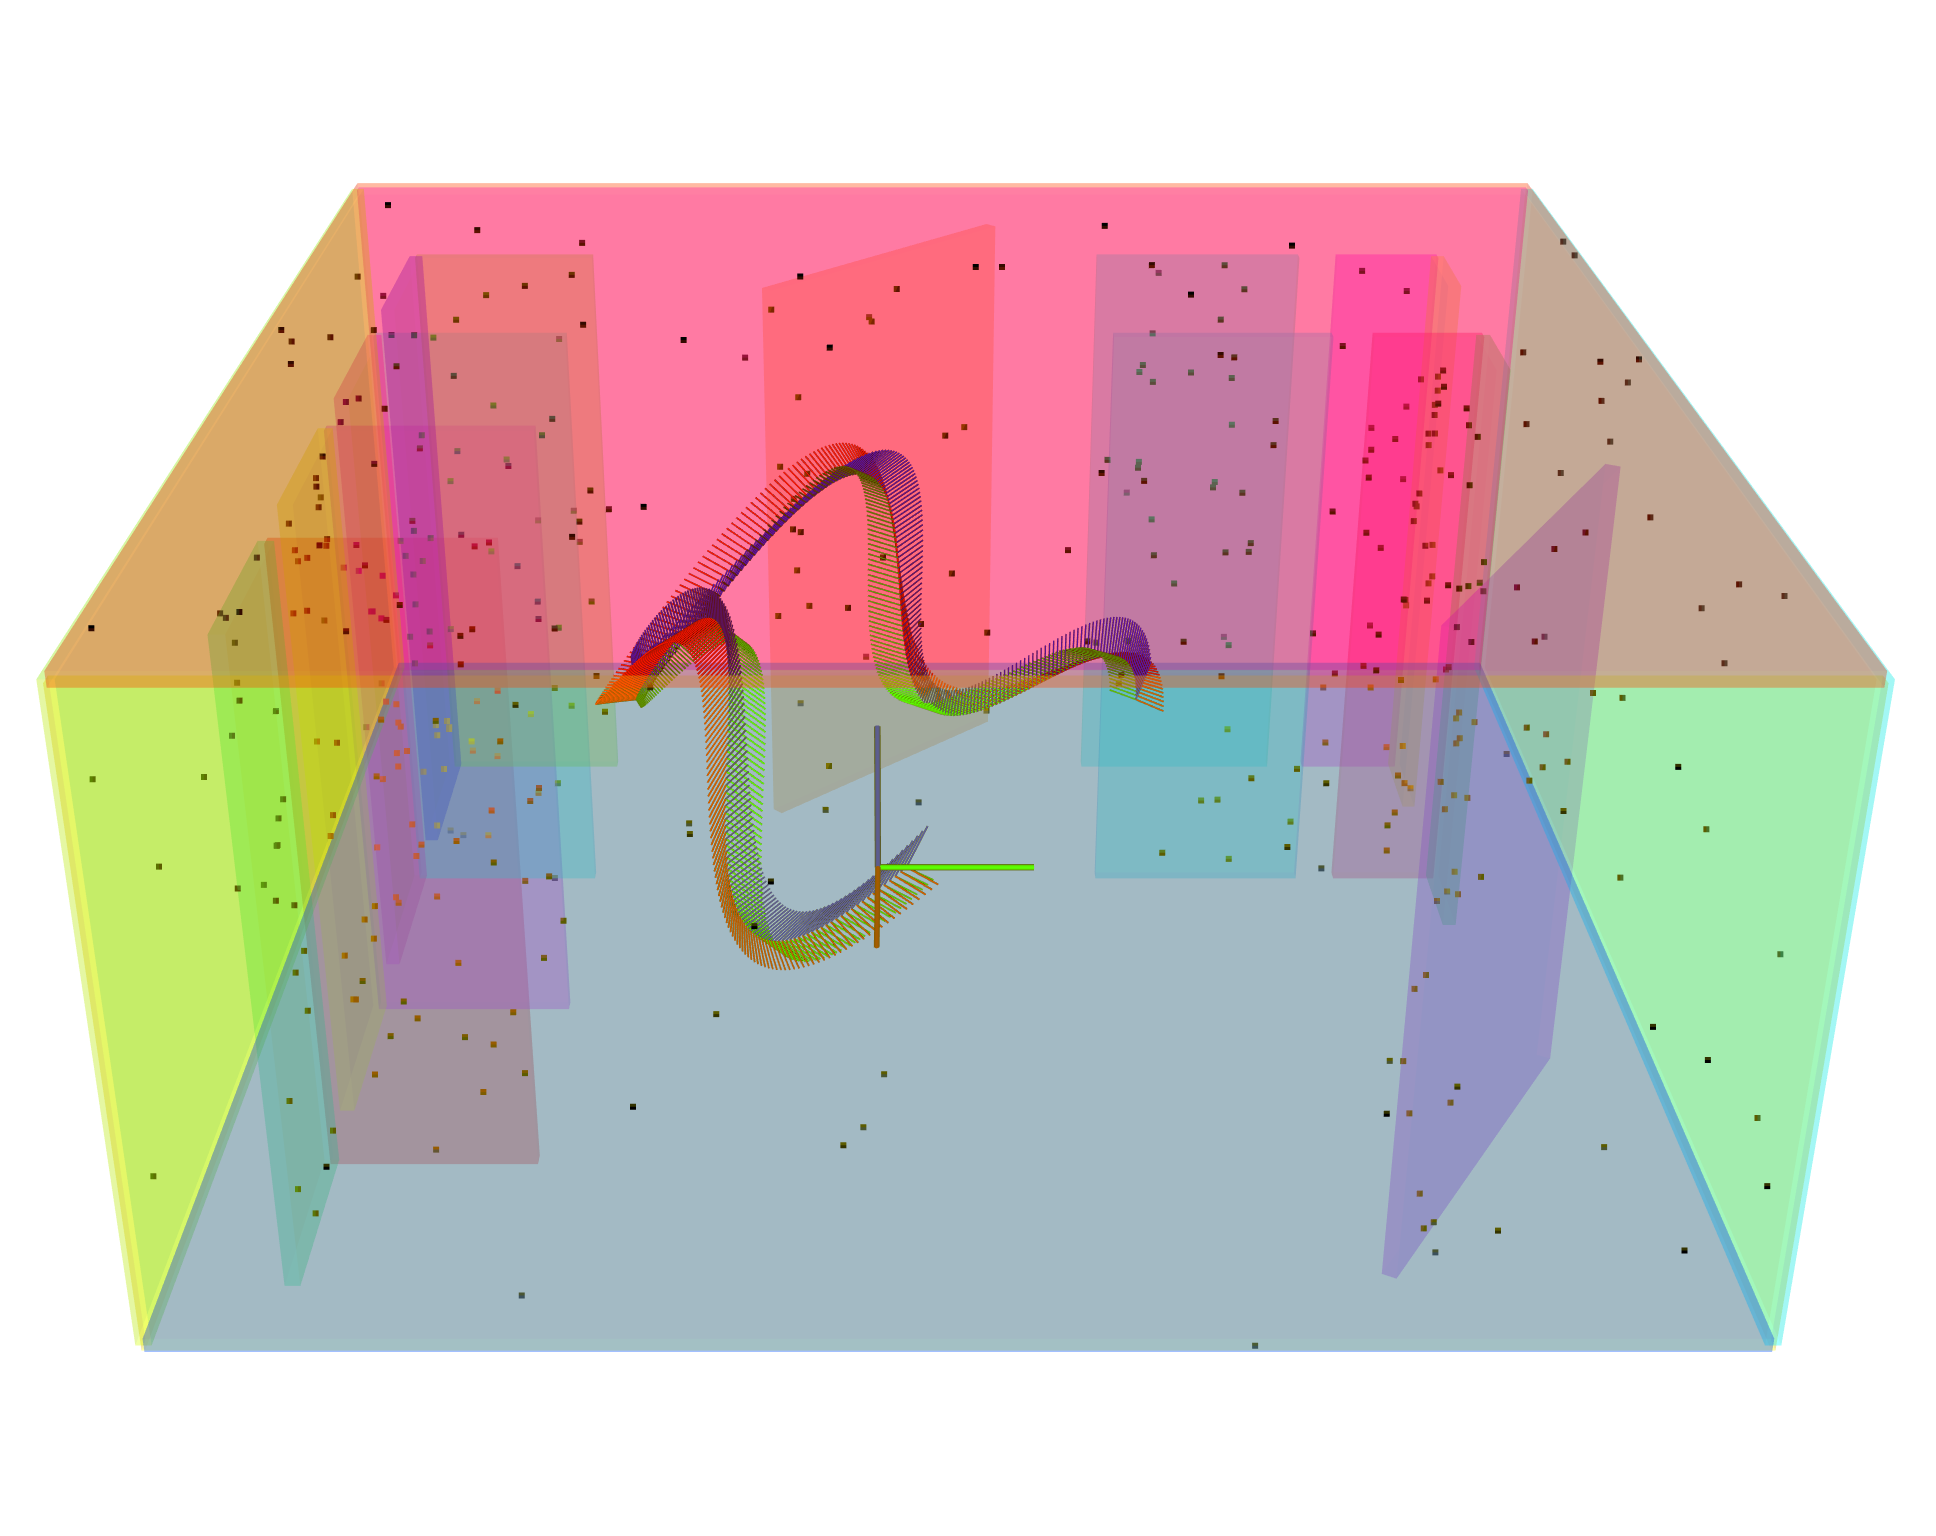
\includegraphics[width=0.48\linewidth]{img/simu/scene1.png}
      \label{fig:simu1}
    }
    \subfigure[\normf{俯视图}]{
      \centering
      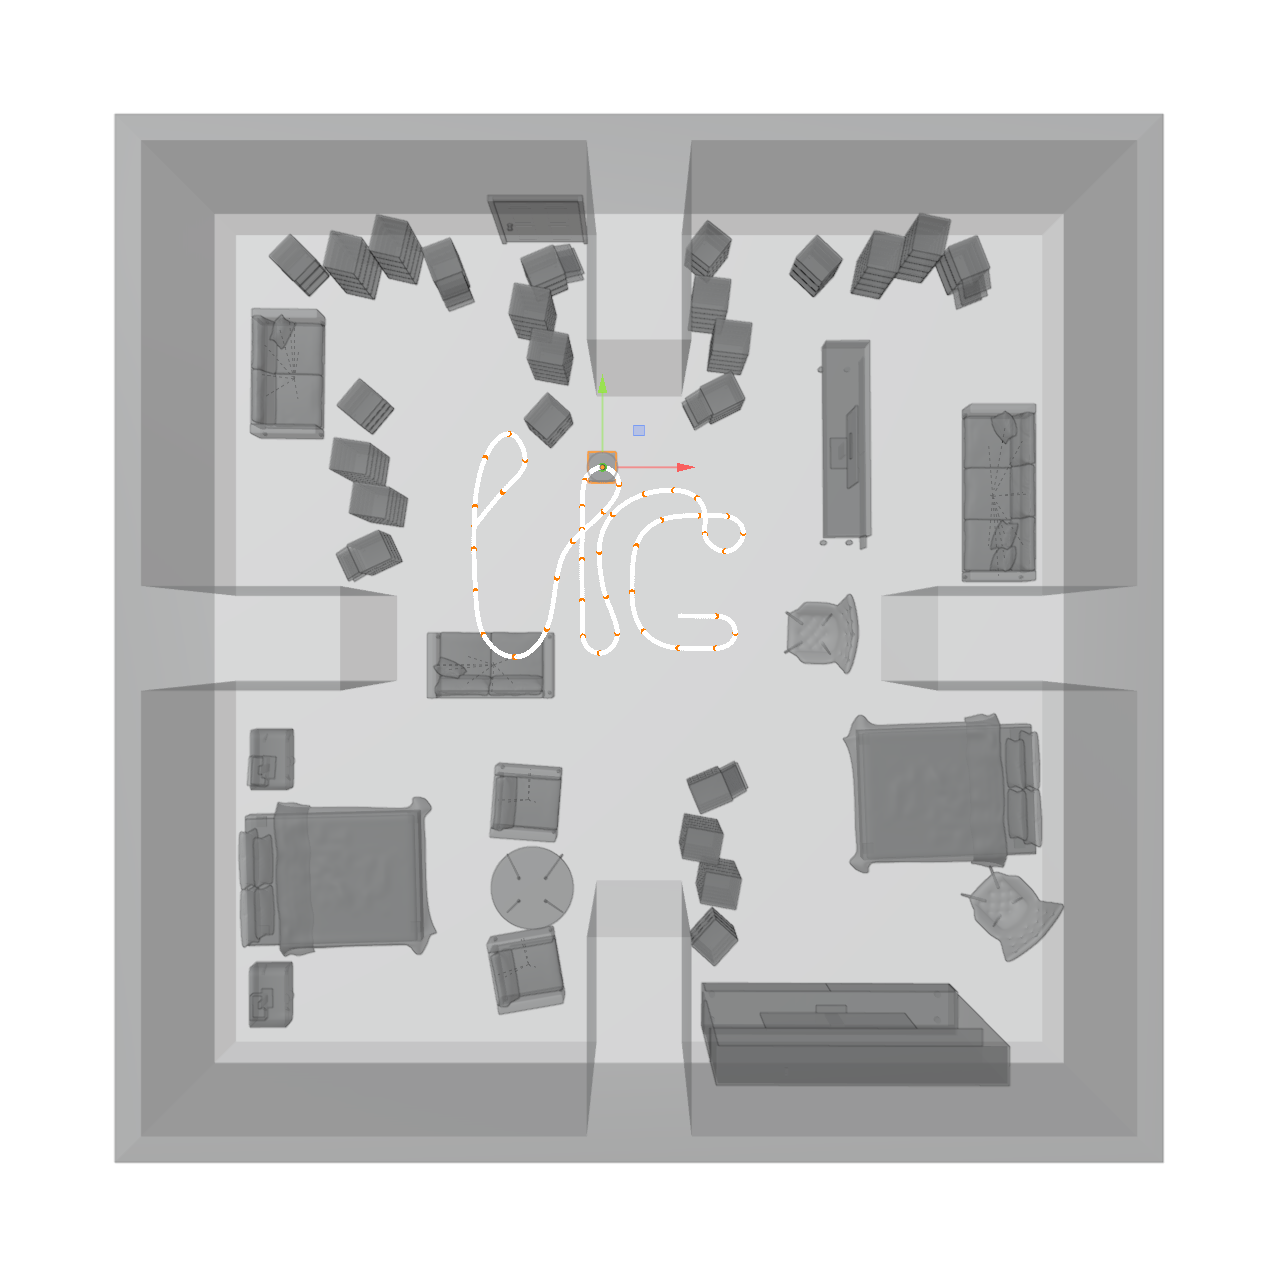
\includegraphics[width=0.48\linewidth]{img/simu/scene2.png}
      \label{fig:simu2}
    }

    \caption{\normf{仿真实验中模拟的场景和轨迹}}

    \label{fig:simu}
  \end{figure}
}

\subsection{\normf{仿真场景的搭建}}
\label{sec:exp_simu}
在仿真实验环节,我们基于GAZEBO\footnote{\normf{GAZEBO官网:\url{https://classic.gazebosim.org}。}}和ROS-Noetic\footnote{\normf{ROS官网:\url{https://www.ros.org}。}}平台进行了场景的构建和轨迹的模拟,并获取了各仿真传感器的原始数据帧序列和真实位姿轨迹。具体而言,我们搭建了一个如图\ref{fig:simu}所示的大小为$10\times 10\times 5\; m^3$、存在多个平面的的封闭环境,同时模拟了一个在空间中被充分激励、时长为$7\;s$的运动轨迹。在图中,离散坐标系序列表示模拟的轨迹;黑点表示模拟的路标点,用于重投影约束的构建。仿真实验中相关传感器的配置与实测实验相同,如传感器噪声、采样频率等,具体内容见\ref{sec:exp_real_world}节。

与图\ref{fig:system}所描述的处理流程一致,在标定的时候会依次进行初始化、数据关联和批处理优化步骤,且后两步会交替进行多次,直至算法收敛为止。解算结果如图\ref{fig:simu_result}所示。其中,图\ref{fig:simu_map}为最终的点云地图;图\ref{fig:simu_plane}为最终的点到面数据关联地图,图中同一颜色的点集构成一个面特征;两地图中的三条轨迹依次为LiDAR离散位姿轨迹(蓝色)、Camera离散位姿轨迹(绿色)和IMU离散位姿轨迹(红色)。
%%%%%%%%%%%%%%%%%%%%%%%%%%%%%%%%%%%%%%%%%%%%%%%%%%%%%%%%%%%%%%%%%%%%%%%%%%%%%%%%%%%%%%%%%
\mlcomment{
  \begin{figure}[htbp]
    \centering

    \subfigure[\normf{带有路标的点云地图}]{
      \centering
      \includegraphics[width=0.48\linewidth]{img/simu/map.png}
      \label{fig:simu_map}
    }
    \subfigure[\normf{带有路标的平面地图}]{
      \centering
      \includegraphics[width=0.48\linewidth]{img/simu/plane.png}
      \label{fig:simu_plane}
    }

    \caption{\normf{仿真实验处理结果}}

    \label{fig:simu_result}
  \end{figure}
}

\subsection{\normf{仿真场景下的算法验证}}
为了分析算法的可行性和收敛特性,对不同迭代次数下的IMU/LiDAR和IMU/Camera的外参和时延估值进行统计,并绘制相应参量的绝对误差曲线
\footnote{\normf{对于标量$x$而言,绝对误差$\delta {x}$即参数估值$\widehat{{x}}$与真实值${x}$差值的绝对值,即有$\delta {x}= \vert \widehat{x}-{x} \vert$。}},
结果如图\ref{fig:simu_evaluate}所示(在图中,旋转量的绝对误差用欧拉角来表示)。	图中的纵坐标表示相应参量的绝对误差;横坐标表示迭代次数,其中第0次迭代表示参数初始化结果,而后的迭代次数为批处理迭代解算。
%%%%%%%%%%%%%%%%%%%%%%%%%%%%%%%%%%%%%%%%%%%%%%%%%%%%%%%%%%%%%%%%%%%%%%%%%%%%%%%%%%%%%%%%%
\mlcomment{
  \begin{figure}[htbp]

    \centering
    \includegraphics[width=0.95\linewidth]{img/simu/params_iter/abs_error.png}

    \caption{\normf{仿真实验IMU/LiDAR/Camera外参和时延的收敛曲线}}
    \label{fig:simu_evaluate}
  \end{figure}
}

从绝对误差曲线图中不难看到,算法具有可行性和良好的收敛性,具体体现在以下几个方面:
\begin{enumerate}
  \item 初始化过程

        在初始化过程(第0次迭代)中,基于LiDAR轨迹、Camera场景结构和IMU位姿B样条曲线,通过手眼标定方法,计算了待标外参较为准确的初始值。其中:外参中的姿态量初始化精度在$2^\circ$以内;而外参中的位移量由于在初始化阶段置为零向量$\boldsymbol{0}_{3\times 1}$(具体见\ref{subsubsec:init_extri_pos}节),因此第0次迭代中外参位移量的“绝对误差”即为其真值的绝对值。这验证了初始化步骤的必要性和有效性。

  \item 迭代过程

        从第1次迭代开始进行多次数据关联和批处理优化(每次批处理优化包含若干次迭代)。由于本文构建的最小二乘标定问题的非线性较为严重,因此在前20次迭代过程中,参数的估值波动较大。在之后的迭代次数中,参数绝对误差不断减小,最后趋于零。这验证了点到面约束和重投影约束的严密性。

  \item 迭代结果

        算法收敛时的参数绝对误差均较小,欧拉角形式表达的外参姿态量的绝对误差在$0.1^\circ$以内,位移量的绝对误差保持在$5\;mm$以内,时延的绝对误差保持在$0.1\;ms$以内。这验证了算法的可行性和正确性。
\end{enumerate}

另外,对于时延的估计而言,在前几次迭代中我们进行LiDAR和IMU之间的时延${^{I}t_{L}}$的优化,但不进行Camera和IMU之间的时延${^{I}t_{C}}$的优化,因此时延参数${^{I}t_{C}}$的绝对误差保持不变。原因在于,与Camera相关的重投影约束相较于与LiDAR相关的点到面约束,有着更强的非线性特性。而时延参数的估计对此是敏感的,在其他参数没有较好收敛的情况下直接进行时延估计是不利于问题的优化求解的。

\section{\normf{实测实验}}
\label{sec:exp_real_world}
\subsection{\normf{多传感器标定实验平台}}

为了对所提出的算法进行综合的测试和评估,我们基于自主搭建的设备平台进行了实测实验。搭建的设备如图\ref{fig:equipment}所示。该平台装备了一个32线的Velodyne\footnote{\normf{Velodyne官网:\url{https://velodynelidar.com}。}}激光雷达VLP-32(图中蓝色方框),具体的参数如表\ref{tab:vlp32}所示;一个BFS-PGE-120S4C-CS\footnote{\normf{FLIR官网:\url{https://www.flir.com}。}}型号的卷帘快门相机(图中绿色方框),具体的参数如表\ref{tab:camera}所示;一个MEMS级别的ADIS-16480  IMU\footnote{\normf{ADI官网:\url{https://www.analog.com/en/index.html}。}}(图中红色方框),具体的参数如表\ref{tab:imu}所示。设备通过GNSS产生PPS(Pluse Per Second)来触发相机和LiDAR,实现不同传感器时间的初步同步。不同传感器通过刚性材料进行连接,以保证刚体变换。Camera/IMU外参真值通过\cite{li2022accurate}获取,LiDAR/IMU外参真值通过开源的Autoware\footnote{\normf{Autoware官网:\url{https://www.autoware.org}。}}工具箱线下标定获取。

%%%%%%%%%%%%%%%%%%%%%%%%%%%%%%%%%%%%%%%%%%%%%%%%%%%%%%%%%%%%%%%%%%%%%%%%%%%%%%%%%%%%%%%%%
\mlcomment{
  \begin{figure}[h]
    \centering

    \subfigure[\normf{自主搭建的实验平台}]{
      \centering
      \begin{minipage}{0.397\linewidth}
        \centerline{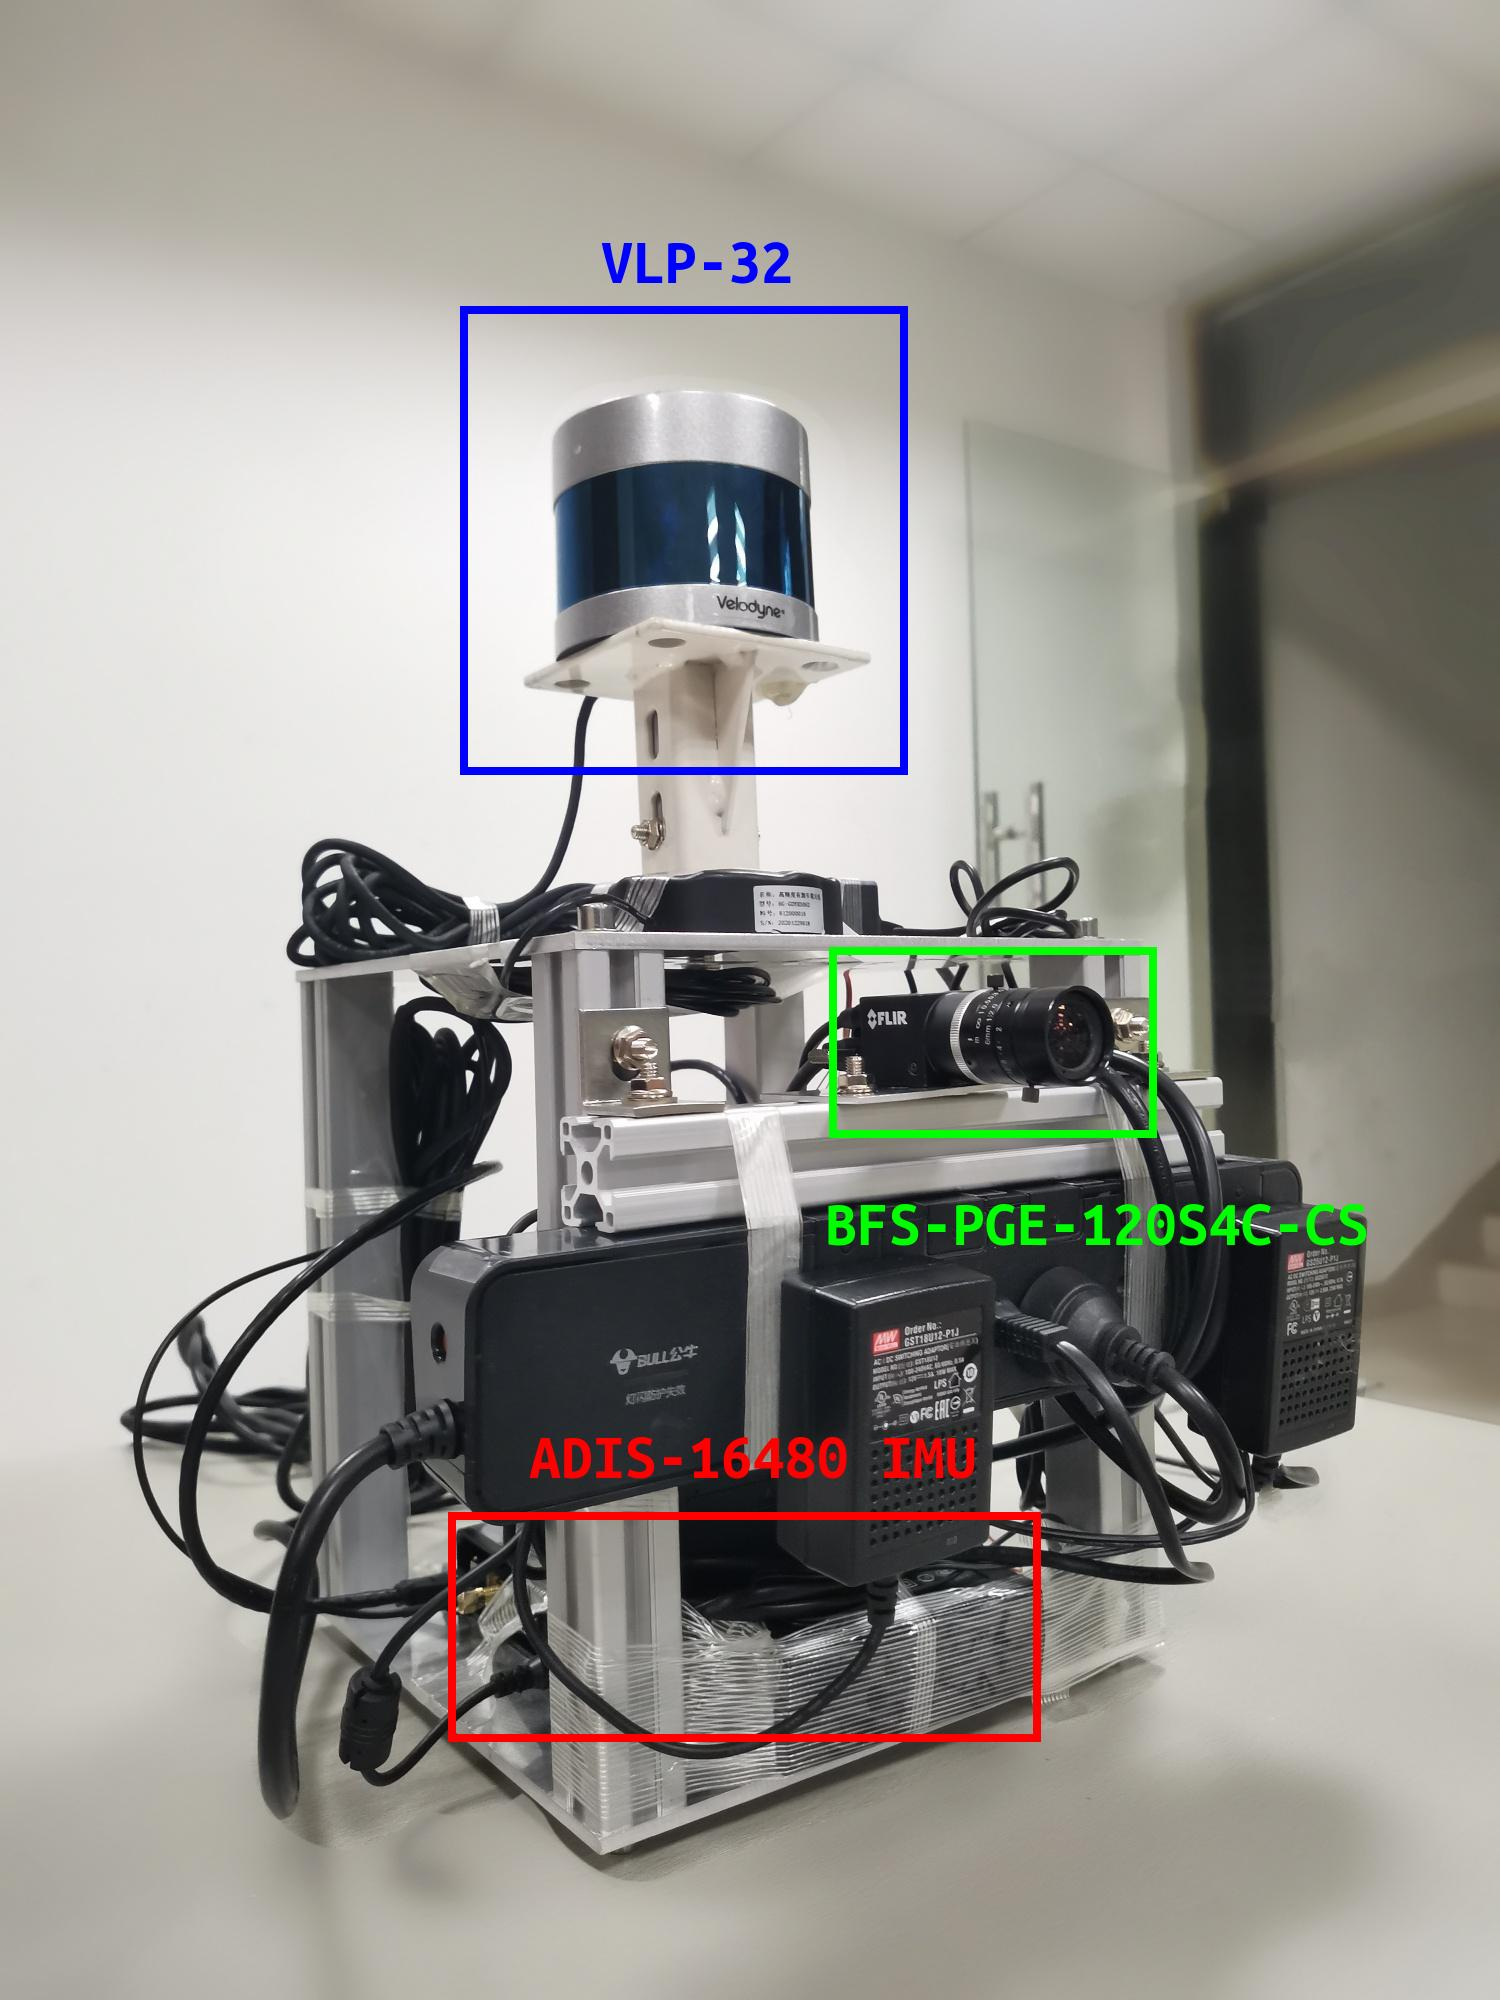
\includegraphics[width=\textwidth]{img/equipment3.jpg}}
        \vspace{20pt}
      \end{minipage}
      \label{fig:equipment}
    }
    \subfigure[\normf{实验场景:室内(上)和室外(下)}]{
      \centering
      \begin{minipage}{0.34\linewidth}
        \centerline{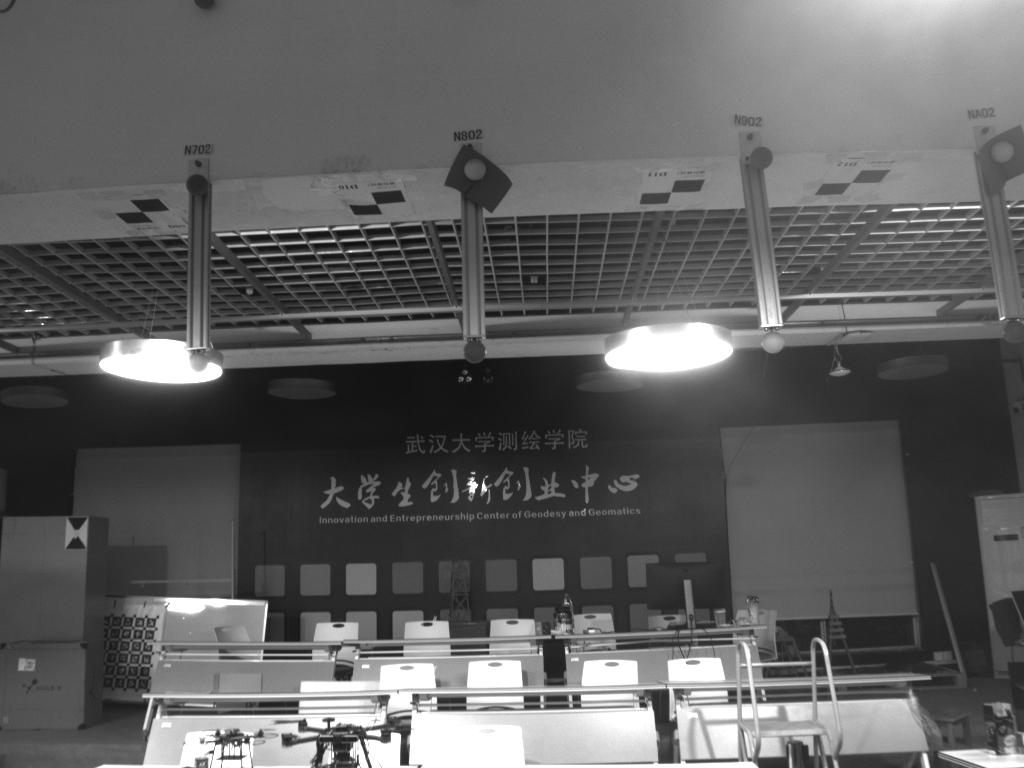
\includegraphics[width=\textwidth]{img/indoor.jpg}}
        \vspace{10pt}
        \centerline{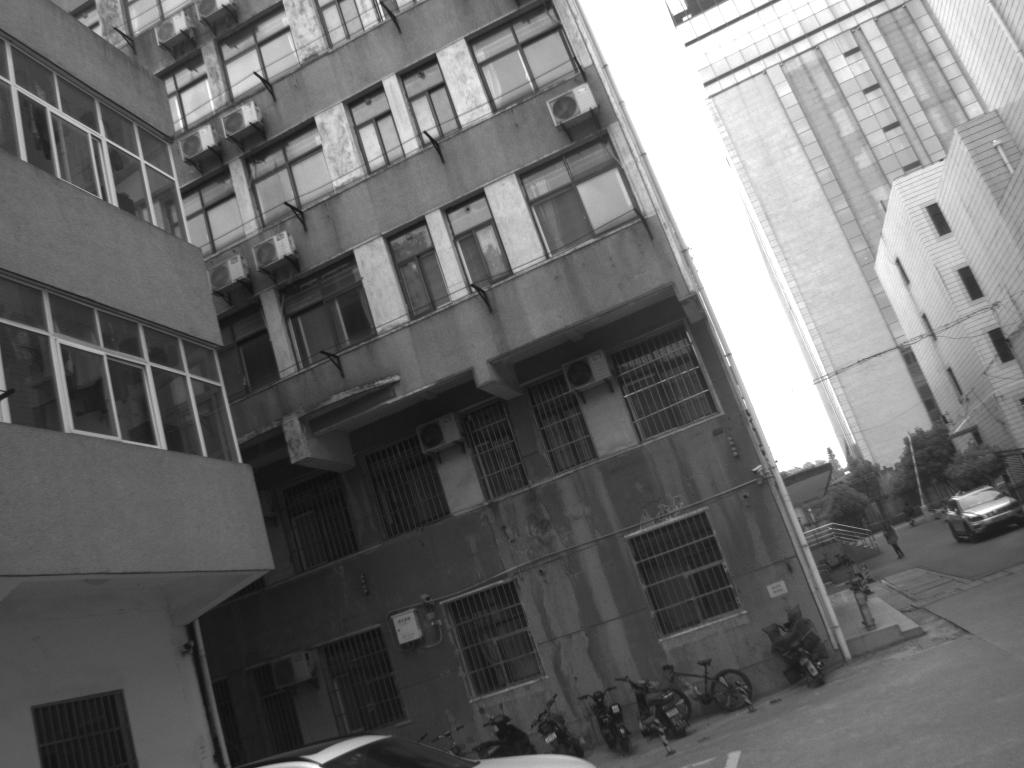
\includegraphics[width=\textwidth]{img/outdoor.jpg}}
        \vspace{20pt}
      \end{minipage}
      \label{fig:scene}
    }
    \caption{\normf{实测实验设备和场景}}
    \label{fig:simu_expr}
  \end{figure}
}
\begin{table*}[htbp]
  \centering
  \normf
  \begin{tabular}{c|ccccc}
    \hline
    {技术参数} & {线束} & {最大测距} & {测量精度} & {视场角(垂直/水平)}     & {角分辨率(垂直/水平)} \\ \hline
    {VLP-32}   & $32$   & $200\;m$   & $\pm5\;cm$ & $+15.0°\sim-25.0°/360°$ & $0.33°/0.1°\sim0.4°$  \\
    \hline
  \end{tabular}
  \caption{\normf{Velodyne VLP-32基本参数}}
  \label{tab:vlp32}
\end{table*}
\begin{table*}[htbp]
  \centering
  \normf
  \begin{tabular}{c|cccc}
    \hline
    {技术参数}             & {快门类型}            & {像素大小} & {图像尺寸} & {最高帧频} \\ \hline
    {BFS-PGE-120S4C-CS}    &
    Rolling                & $
    1.85\times1.85\;\mu m$ & $1024\times768${像素} & 30HZ                                 \\ 	\hline
  \end{tabular}
  \caption{\normf{BFS-PGE-120S4C-CS基本参数}}
  \label{tab:camera}
\end{table*}
\begin{table*}[htbp]
  \centering
  \normf
  \begin{tabular}{c|cccc}
    \hline
    {技术参数}   & {陀螺仪零偏} & {加速度计零偏} & {速度随机游走}       & {角度随机游走}    \\ \hline
    {ADIS-16480} & $8\;°/h$     & $1500\;mGal$   & $0.18\;m/s/\sqrt{h}$ & $0.3\;°/\sqrt{h}$ \\ 	\hline
  \end{tabular}
  \caption{\normf{ADIS-16480 IMU基本参数}}
  \label{tab:imu}
\end{table*}

\subsection{\normf{室内外典型场景下的算法测试和评估}}
为了让实验更具代表性,本文分别选取了室内外两个典型场景进行了标定实验,如图\ref{fig:scene}所示。在数据采集过程中,LiDAR、Camera和IMU的采样频率分别设置为10HZ、10HZ和400HZ。对于室内和室外场景下的标定解算,我们均使用了$25\;s$的数据序列,标定结果如图\ref{fig:real_world_result}所示。
%%%%%%%%%%%%%%%%%%%%%%%%%%%%%%%%%%%%%%%%%%%%%%%%%%%%%%%%%%%%%%%%%%%%%%%%%%%%%%%%%%%%%%%%%
\mlcomment{
  \begin{figure}[h]
    \centering

    \subfigure[\normf{室内}]{
      \centering
      \begin{minipage}{0.37\linewidth}
        \centerline{\includegraphics[width=\textwidth]{img/real_world/indoor/map.png}}
        \vspace{10pt}
        \centerline{\includegraphics[width=\textwidth]{img/real_world/indoor/plane.png}}
        \vspace{20pt}
      \end{minipage}
      \label{fig:scene_indoor}
    }
    \subfigure[\normf{室外}]{
      \centering
      \begin{minipage}{0.37\linewidth}
        \centerline{\includegraphics[width=\textwidth]{img/real_world/outdoor/map.png}}
        \vspace{10pt}
        \centerline{\includegraphics[width=\textwidth]{img/real_world/outdoor/plane.png}}
        \vspace{20pt}
      \end{minipage}
      \label{fig:scene_outdoor}
    }
    \subfigure[\normf{标定结果可视化}]{
      \centering
      \begin{minipage}{0.184\linewidth}
        \centerline{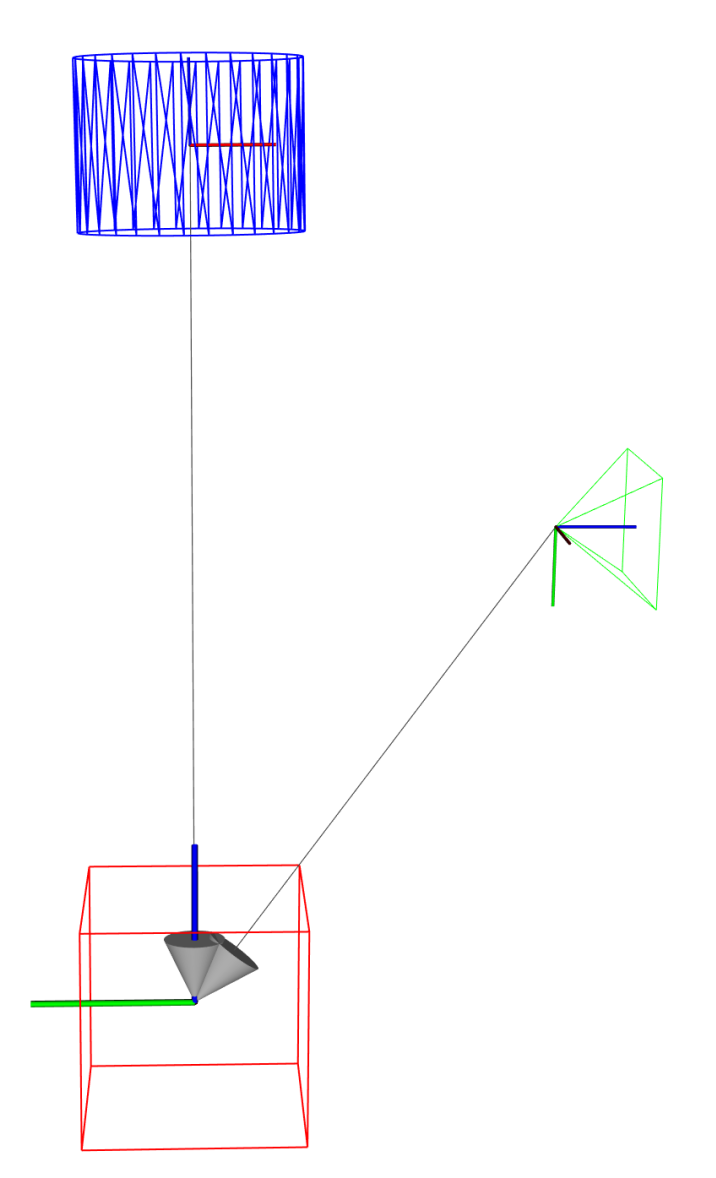
\includegraphics[width=\textwidth]{img/real_world/sensors1.png}}
        \vspace{10pt}
        \centerline{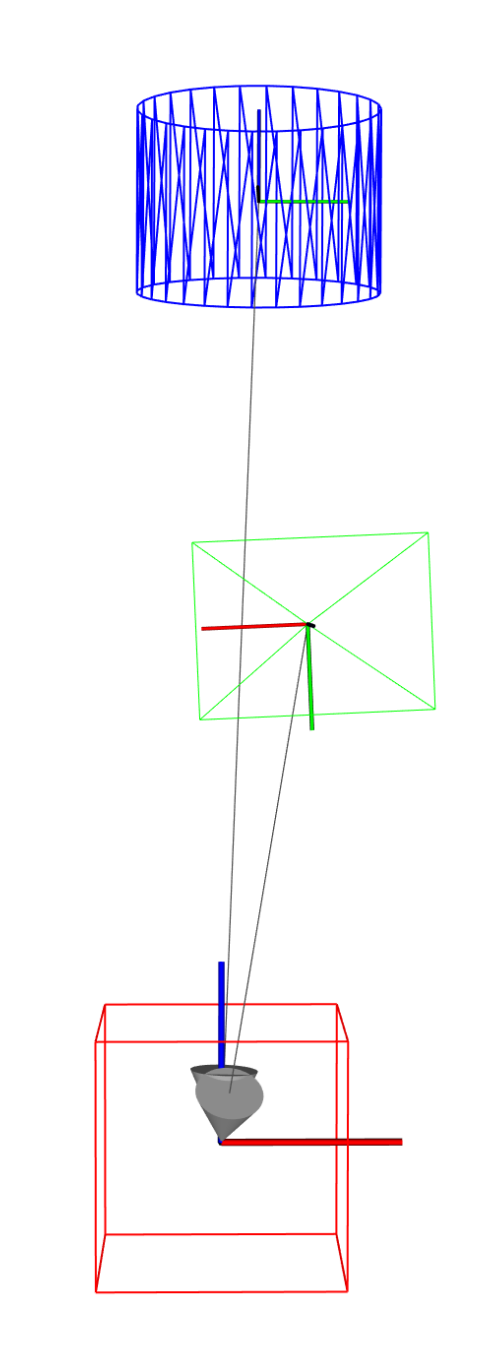
\includegraphics[width=\textwidth]{img/real_world/sensors2.png}}
        \vspace{20pt}
      \end{minipage}
      \label{fig:sensors}
    }
    \caption{\normf{实测实验解算结果}}
    \label{fig:real_world_result}
  \end{figure}
}

在实际进行解算的时候,为了保证迭代优化解算时的可靠性,避免系统陷入局部最优,我们使用了如下所述的优化策略:在首次批处理优化中,我们选择优化位姿B样条曲线和外参,同时考虑到相机尺度因子可能受到不准确相机位姿序列的影响而造成初始化不精确,该参数也会被加入到图中进行优化。其他参数在首次批处理中被固定,不进行优化。在之后的批处理优化中,我们会依次将相机内参、IMU内参加入到优化图中。最后,我们会加入时延参数进行优化,因为时参的估计易受其他未校准参数的影响。注意到,IMU位姿B样条曲线在所有的批处理中均被加入到图中优化,以为下一次的数据关联提供更为精确的先验信息。正如\ref{subsec:alg_define}节所述,我们在批处理中引入了优化选项,可以在不影响参数可观性的前提下,选择性的标定部分参数,因此上述的优化策略是易于实现的。

%%%%%%%%%%%%%%%%%%%%%%%%%%%%%%%%%%%%%%%%%%%%%%%%%%%%%%%%%%%%%%%%%%%%%%%%%%%%%%%%%%%%%%%%%
\mlcomment{
  \begin{figure}[htbp]
    \centering
    \includegraphics[width=0.95\linewidth]{img/real_world/indoor/params_iter/abs_error.png}

    \caption{\normf{室内实测实验IMU/LiDAR/Camera外参和时延的收敛曲线}}

    \label{fig:indoor_evaluate}
  \end{figure}
}
%%%%%%%%%%%%%%%%%%%%%%%%%%%%%%%%%%%%%%%%%%%%%%%%%%%%%%%%%%%%%%%%%%%%%%%%%%%%%%%%%%%%%%%%%
\mlcomment{
  \begin{figure}[htbp]
    \centering
    \includegraphics[width=0.95\linewidth]{img/real_world/outdoor/params_iter/abs_error.png}

    \caption{\normf{室外实测实验IMU/LiDAR/Camera外参和时延的收敛曲线}}

    \label{fig:outdoor_evaluate}
  \end{figure}
}
% Please add the following required packages to your document preamble:
% \usepackage{multirow}
\begin{table}[]
  \centering
  \normf
  \begin{tabular}{c|c|ccccccc}
    \hline
    \multirow{2}{*}{场景} & \multirow{2}{*}{参数} & \multicolumn{3}{c|}{外参姿态误差$(^\circ)$} & \multicolumn{3}{c|}{外参位移误差$(mm)$} & 时延$(ms)$                                                                                                                                                                    \\ \cline{3-9}
                          &                       & $\delta{\boldsymbol{\theta}(r)}$            & $\delta{\boldsymbol{\theta}(p)}$        & \multicolumn{1}{c|}{$\delta{\boldsymbol{\theta}(y)}$} & $\delta{\boldsymbol{p}(x)}$ & $\delta{\boldsymbol{p}(y)}$ & \multicolumn{1}{c|}{$\delta{\boldsymbol{p}(z)}$} & $ t$   \\ \hline
    \multirow{2}{*}{室内} & IMU/LiDAR             & 0.012                                       & 0.005                                   & 0.044                                                 & 0.374                       & 1.868                       & 0.964                                            & 5.822  \\
                          & IMU/Camera            & 0.089                                       & 0.049                                   & 0.009                                                 & 1.596                       & 2.237                       & 2.207                                            & 12.928 \\ \hline
    \multirow{2}{*}{室外} & IMU/LiDAR             & 0.034                                       & 0.043                                   & 0.015                                                 & 1.646                       & 1.862                       & 2.314                                            & 5.734  \\
                          & IMU/Camera            & 0.064                                       & 0.006                                   & 0.030                                                 & 4.774                       & 0.888                       & 4.867                                            & 6.476  \\ \hline
  \end{tabular}
  \caption{\normf{实测实验外参标定误差及时延估值}}
  \label{tab:real_world_statistic}
\end{table}

与仿真实验类似,我们对室内外实验标定过程中不同迭代次数下的外参和时延的估值进行了统计,并绘制了相应的绝对误差曲线,结果如图\ref{fig:indoor_evaluate}、\ref{fig:outdoor_evaluate}所示,图中横、纵坐标的含义与仿真实验一致。由于无法获得时延参数的真值,因此我们绘制了其状态变化曲线。可以看到,无论是室内环境还是室外环境,基于手眼标定法初始化的IMU/LiDAR和IMU/Camera外参的精度能够得到保证,尤其是IMU/Camera外参姿态量,其初始化后的偏差比IMU/LiDAR外参姿态量的初始化偏差小很多,这离不开SfM算法的鲁棒性。同时,相较于仿真实验,实测实验在前20次迭代计算中参数的波动更小,收敛特性更好。原因在于,在实测实验数据采集时我们充分激励载体运动,同时在解算时使用了更长时间的数据序列,二者对于标定问题的解算都是有利的。在算法收敛时,外参姿态量的偏差在$0.1^\circ$以内,位移量偏差在$5\;mm$以内,如表\ref{tab:real_world_statistic}所示。

同时注意到,相比与IMU/LiDAR参数的估计迭代过程,IMU/Camera相关参数在迭代过程中波动更大。原因在于,为了对SfM算法估计的场景结构进行精化,在迭代过程中我们将特征点逆深度参数向量加入到优化图中,高维数的逆深度参数向量会让图优化问题中的非线性特性变得更加严重,导致迭代求解不稳定。好在通过多次迭代线性化操作后,参数最后都会收敛到一个较优的值。
另外我们注意到,在室内、室外不同环境下,IMU/Camera的时延参数收敛值不一样:在室内环境下,相机相对于IMU的时延${^I}t_C$的估值为$12.928\;ms$,而在室外环境下,该时延参数估值为$6.476\;ms$。原因在于相较于光线充足的室外环境,室内环境光线不足,相机需要更长的曝光时间。

为了考察室内外场景下算法的收敛特征,我们对批处理优化过程中的目标函数、梯度和置信半径进行统计,并绘制了如图\ref{fig:real_world_iter_info}所示的变化曲线\footnote{\normf{图中目标函数和梯度的变化曲线已通过$\log_{10}(\cdot)$函数映射。}},其中:
\begin{enumerate}
  \item 目标函数变化曲线

        该表征了优化过程中的损失变化和收敛速度,算法损失下降越快,相应的收敛速度就越快。从图中可以看出,无论是室内场景还是室外场景,算法收敛速度较快,目标函数都能在第一次批处理优化后(BO 1)达到较小的值。

  \item 梯度变化曲线

        该曲线与优化过程中算法逼近最优解的表现相关,算法越逼近最优解,梯度越小。需要注意的是,算法无论逼近的是局部最优解还是全局最优解,对应的梯度都小。由于在每次批处理优化后都会重新进行数据关联,因此图中相邻批处理优化之间的梯度存在跳跃。从图中可以看到,每次批处理优化结束时的梯度都较小,结合目标函数变化曲线,可以说明算法能够求解得到全局最优解。

  \item 置信半径变化曲线

        由于本文使用LM法进行优化,因此我们绘制了置信半径变化曲线。置信半径$1/\lambda$
        的大小体现了LM法在迭代求解时的“自信度”,具体表现在参数更新步长方面,具体参考附录\ref{appendix:lm_alg}。从图中可以看出,由于每次批处理优化的目标函数均在减小,因此置信半径在不断增大。
\end{enumerate}
%%%%%%%%%%%%%%%%%%%%%%%%%%%%%%%%%%%%%%%%%%%%%%%%%%%%%%%%%%%%%%%%%%%%%%%%%%%%%%%%%%%%%%%%%
\mlcomment{
  \begin{figure}[htbp]
    \centering
    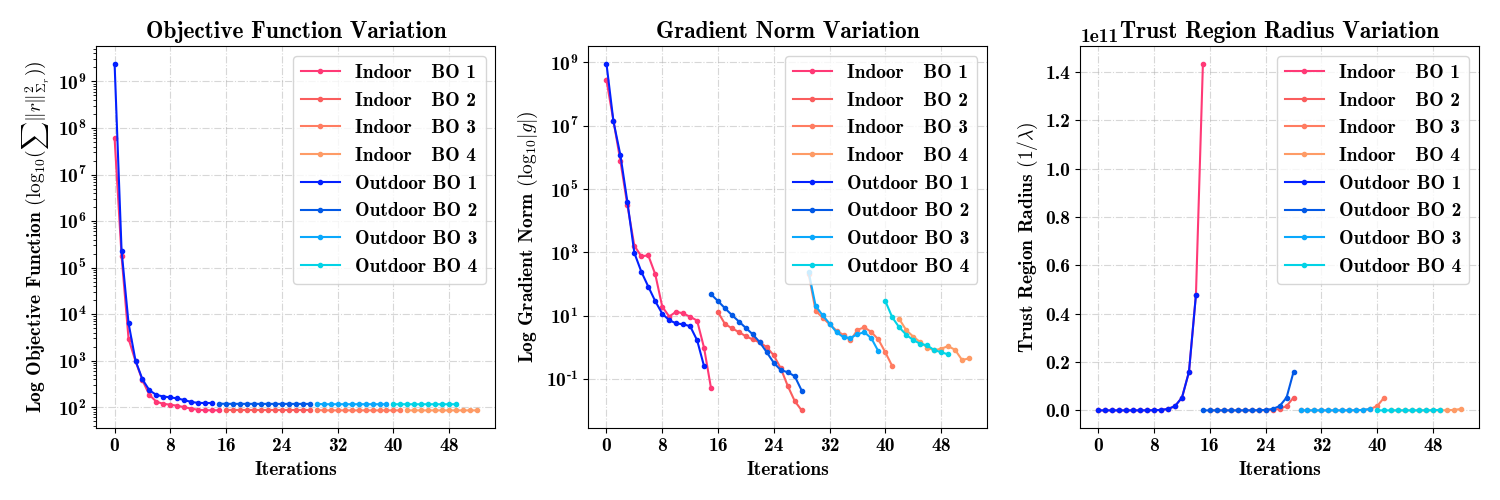
\includegraphics[width=0.95\linewidth]{img/real_world/iter_info.png}

    \caption{\normf{实测实验批处理优化中的目标函数(左)、梯度(中)和置信半径(右)变化曲线}}

    \label{fig:real_world_iter_info}
  \end{figure}
}

为了考察约束构建准确性和有效性,我们对每次批处理优化时的残差进行统计,并绘制了如图\ref{fig:real_world_residuals}所示的残差分布图。在批处理涉及的三种约束中,点到面约束和IMU/LiDAR相关参数有关,重投影约束和IMU/Camera相关参数有关,因此在分析过程中主要考虑了这两种约束对应的残差分布。从图中可以看到,无论是室内场景还是室外场景,点到面残差和重投影残差呈现零均值正态分布,并且随着批处理优化次数的增加,标准差更小,这说明了约束构建的正确性和批处理优化的有效性。同时可以发现,在第一次批处理优化后,构建的点到面约束明显增加,原因在于经过该次批处理优化,IMU/LiDAR外参中的位移量被估计,能够更好的去除点云帧中的运动畸变,从而找到更多的面特征,以构建更多、更强的点到面约束。

\mlcomment{
  \begin{figure}[htbp]
    \centering

    \subfigure[\normf{室内实验}]{
      \centering
      \includegraphics[width=0.95\linewidth]{img/real_world/indoor/residuals.png}
    }
    \subfigure[\normf{室外实验}]{
      \centering
      \includegraphics[width=0.95\linewidth]{img/real_world/outdoor/residuals.png}
    }

    \caption{\normf{批处理优化过程中的点到面残差和重投影残差分布}}

    \label{fig:real_world_residuals}
  \end{figure}
}

\subsection{\normf{算法一致性评价}}
为了更为直观的评价算法的一致性,我们基于解算完成后的IMU位姿B样条曲线$\mathcal{B}$、LiDAR点云地图$\mathcal{M}$和相机图像序列$\mathcal{C}_{\mathcal{I}}$,将灰度信息映射到点云地图上,得到了如图\ref{fig:indoor_pointcloud}、图\ref{fig:outdoor_pointcloud}所示的重建场景$\mathcal{M}^\prime$。结果点云地图$\mathcal{M}^\prime$相较于原始输入的LiDAR点云地图$\mathcal{M}$,附带有灰度信息。因此,通过$\mathcal{M}^\prime$能够比较直观的查看地图几何结构和灰度属性之间的对应关系,从而对算法的一致性进行评价。具体来说,对于点$\boldsymbol{p}\in\mathcal{M}$,查询能够正常观察到该点的图像序列,并通过采样构造灰度向量。为了让场景亮度具有一致性,我们将该灰度向量的均值作为该点的灰度,处理流程如算法\ref{alg:color_map}所示。
\begin{algorithm}[htbp]
  \label{alg:color_map}
  \caption{\normf{构建带有灰度纹理的三维场景}}
  \LinesNumbered 
  \KwIn{\normf{IMU位姿B样条曲线$\mathcal{B}$、LiDAR点云地图$\mathcal{M}$和相机图像序列$\mathcal{C}_{\mathcal{I}}$}}%输入参数
  \KwOut{\normf{带有灰度纹理的三维场景$\mathcal{M}^\prime$}}
  \ForEach{$\boldsymbol{p}\in\mathcal{M}$}{
    \normf{初始化灰度集合:}$\mathcal{G}_{\boldsymbol{p}}=\left\lbrace \right\rbrace $\;
    \ForEach{$i\in\left( \mathcal{C}_{\mathcal{I}}\right) ^\dagger$}{
      \normf{将点变换到第$i$个相机坐标系下:}
      $\boldsymbol{p}^\prime\gets\begin{pmatrix}
      \boldsymbol{p}^\prime\\1			\end{pmatrix}={{^{I}_{C}}\boldsymbol{T}^{-1}}\cdot{{^{I_0}_{I}}\boldsymbol{T}^{-1}\left( t_{C_i}+{^{I}t_C}\right) }\cdot{{^{I_0}_{I}}\boldsymbol{T}\left( t_{L}(\boldsymbol{p})+{^{I}t_L}\right) }\cdot{{^{I}_{L}}\boldsymbol{T}}\begin{pmatrix}
      \boldsymbol{p}\\1
      \end{pmatrix}$\;
      
      \If{$\boldsymbol{p}^\prime_z>0\;\boldsymbol{\&}\;\pi(\boldsymbol{p}^\prime)\in\mathcal{C}_{\mathcal{I}_i}$}{
        \normf{记录能被正常观测得到的点的灰度:}
        $\mathcal{G}_{\boldsymbol{p}}\gets\mathcal{C}_{\mathcal{I}_i}\left( \pi(\boldsymbol{p}^\prime)\right) $\;
      }
    }
    \If{$\mathcal{G}_{\boldsymbol{p}}\neq\boldsymbol{\varnothing}$}{
      $c=0,\;g_s=0$\;
      \ForEach{$g\in\mathcal{G}_{\boldsymbol{p}}$}{
        $g_s=g_s+g,\;c=c+1$\;
      }
      \normf{记录点及其灰度均值:}
      $\mathcal{M}^\prime\gets\left\lbrace \boldsymbol{p}\mid g_s/c\right\rbrace $\;
    }
  }	
\end{algorithm}

反过来,我们通过类似的处理,将点云投射到影像上,结果如图\ref{fig:indoor_view}、图\ref{fig:outdoor_view}所示,图中不同颜色代表不同深度。从图\ref{fig:pointcloud}中可以看到,无论是室内场景还是室外场景,重建的结果都有较高的一致性,主要体现在:
\begin{enumerate}
  \item 重建的点云地图结构和灰度地图一致。在灰度映射的点云地图中,几何结构和灰度信息对应得较好,如室内场景中标牌上的文字能够被清晰的重建出来。
  
  \item 重建的点云地图相对结构一致。如室外场景中位于过道上的门窗排列一致,过道前不同停车位之间的几何连接是一致的。
  
  \item “深度”影像的物体和原始影像上同名物体之间的几何位置对应得很好。
\end{enumerate}

综上可见,本文所提出的基于连续时间的LiDAR/Camera/IMU的时空标定方法能够在保证整个标定系统一致的条件下,求得全局最优的解。

%%%%%%%%%%%%%%%%%%%%%%%%%%%%%%%%%%%%%%%%%%%%%%%%%%%%%%%%%%%%%%%%%%%%%%%%%%%%%%%%%%%%%%%%%
\mlcomment{	
\begin{figure}[htbp]
  \centering
    \subfigure[\normf{室内上色点云地图}]{
  \centering
    \includegraphics[width=0.4\linewidth]{img/real_world/indoor/pointcloud1.png}
    \includegraphics[width=0.4\linewidth]{img/real_world/indoor/pointcloud2.png}
  \label{fig:indoor_pointcloud}
  }
  \subfigure[\normf{室内共视视角}]{
    \centering
    \includegraphics[width=0.2\linewidth]{img/real_world/indoor/image_view1.png}
    \includegraphics[width=0.2\linewidth]{img/real_world/indoor/map_view1.png}
    \includegraphics[width=0.2\linewidth]{img/real_world/indoor/image_view2.png}
    \includegraphics[width=0.2\linewidth]{img/real_world/indoor/map_view2.png}
    \label{fig:indoor_view}
  }
  \subfigure[\normf{室外上色点云地图}]{
    \centering
    \includegraphics[width=0.4\linewidth]{img/real_world/outdoor/pointcloud1.png}
    \includegraphics[width=0.4\linewidth]{img/real_world/outdoor/pointcloud2.png}
    \label{fig:outdoor_pointcloud}
  }
        \subfigure[\normf{室外共视视角}]{
    \centering
    \includegraphics[width=0.2\linewidth]{img/real_world/outdoor/image_view1.png}
    \includegraphics[width=0.2\linewidth]{img/real_world/outdoor/map_view1.png}
    \includegraphics[width=0.2\linewidth]{img/real_world/outdoor/image_view2.png}
    \includegraphics[width=0.2\linewidth]{img/real_world/outdoor/map_view2.png}
    \label{fig:outdoor_view}
  }
  \caption{\normf{实测实验场景重建}}
  
  \label{fig:pointcloud}
\end{figure}
}

\section{\normf{系统可观性实验}}
\label{appendix:observability}
系统的可观性是指基于系统的有限输入和输出信息,能否唯一确定系统在某个时刻的状态信息的性质\cite{bubnicki2005modern}。当系统的状态能够被完全确定时,称系统可观;当系统的部分状态可以被确定时,称系统部分可观;当系统的状态都不能确定时,称系统不可观。由于本文提出的基于连续时间的LiDAR/Camera/IMU的时空标定方法是一种通过自运动估计的无靶标标定方法,在标定的过程中需要充分的运动激励来保证系统的可观性。如果在标定时载体的运动不充分,会严重损害估计参数的精度,甚至导致参数不可观,无法被估计出来。为此,有必要对系统在不同运动形式下的可观性进行分析和测试。

\subsection{\normf{基于法方程的系统可观性分析}}
如前文所述,本文提出的标定系统是一个基于图优化的标定框架,因此不能像滤波优化方法\cite{huai2022observability}、\cite{mirzaei2008kalman}、\cite{yang2019degenerate}、\cite{lv2022observability}一样,通过能观性秩条件(Observability Rank Condition,ORC)对系统的可观性进行判定。
与滤波优化方法不同,图优化方法在每次迭代中,基于高斯牛顿法或者LM法(本文使用LM法,算法细节见附录\ref{appendix:lm_alg})构建法方程,而后求解该方程并对参数进行增量更新。因此,本文从法方程的角度出发进行系统的可观性分析。在不考虑置信域的情况下,LM方法的法方程如下所示:
\begin{equation}
  \boldsymbol{H}_{n\times n}\cdot\delta\boldsymbol{x}_{n\times 1}=\boldsymbol{b}_{n\times 1}
  \quad
  \mathrm{s.t.}
  \quad
  \begin{cases}
    \begin{aligned}
      \boldsymbol{H}_{n\times n} & =	\left( \frac{\partial^2 \boldsymbol{r}(\boldsymbol{x})}{\partial \boldsymbol{x}^T}\bigg|_{\boldsymbol{x}_{op}}\right)^T
      \left( \frac{\partial^2 \boldsymbol{r}(\boldsymbol{x})}{\partial \boldsymbol{x}}\bigg|_{\boldsymbol{x}_{op}}\right)                                                                       \\
      \boldsymbol{b}_{n\times 1} & =-\left( \frac{\partial^2 \boldsymbol{r}(\boldsymbol{x})}{\partial \boldsymbol{x}^T}\bigg|_{\boldsymbol{x}_{op}}\right)^T\boldsymbol{r}(\boldsymbol{x}_{op})
    \end{aligned}
  \end{cases}
\end{equation}
其中:$\delta\boldsymbol{x}_{n\times1}$为的参数更新向量;$\boldsymbol{x}_{op}$为参数向量的优化初值;$\boldsymbol{r}(\boldsymbol{x})$为损失函数。
为了简洁,对于参数更新向量$\delta\boldsymbol{x}$,我们只考虑系统的外参和时延参数,不考虑其余参数:
\begin{equation}
  \begin{aligned}
    \delta\boldsymbol{x}      & =\left\lbrace
    \delta\boldsymbol{x}_{ex},\delta\boldsymbol{x}_{t}
    \right\rbrace_{14\times 1}                                                                                                                                                                                \\
    \delta\boldsymbol{x}_{ex} & =\left\lbrace \delta{^{I}_{L}\boldsymbol{\theta}},\delta{^{I}}\boldsymbol{p}_{L},\delta{^{I}_{C}\boldsymbol{\theta}},\delta{^{I}}\boldsymbol{p}_{C}\right\rbrace_{12\times 1} \\
    \delta\boldsymbol{x}_{t}  & =\left\lbrace \delta{^{I}t_{L}},\delta{^{I}t_{C}}\right\rbrace_{2\times 1}                                                                                                    \\
  \end{aligned}
\end{equation}
另外,在\ref{sect:batch_optimization}节中批处理优化时涉及的四种因子中,点到面因子与LiDAR的外参和时参求解相关,重投影因子与Camera的外参和时参求解相关,因此令残差向量为:
\begin{equation}
  \boldsymbol{r}_{3\times 1}=\begin{pmatrix}
    \boldsymbol{r}_{ij}^k(l) \\\boldsymbol{r}_{ij}^{mn}(c)
  \end{pmatrix}
  \simeq
  \begin{pmatrix}
    \boldsymbol{r}(l) \\\boldsymbol{r}(c)
  \end{pmatrix}
\end{equation}
则残差$\boldsymbol{r}$对参数$\delta\boldsymbol{x}$的雅克比矩阵为:
\begin{equation}
  \boldsymbol{J}_{\boldsymbol{x}}=\frac{\partial \boldsymbol{r}}{\partial \delta \boldsymbol{x}}=
  \begin{pmatrix}
    \frac{\partial \boldsymbol{r}(l)}{\partial \delta {^{I}_{L}\boldsymbol{\theta}}} &
    \frac{\partial \boldsymbol{r}(l)}{\partial \delta {^{I}\boldsymbol{p}_L}}        &
    \boldsymbol{0}_{1\times 3}                                                       &
    \boldsymbol{0}_{1\times 3}                                                       &
    \frac{\partial \boldsymbol{r}(l)}{\partial \delta {^{I}t_{L}}}                   &
    \boldsymbol{0}_{1\times 1}                                                         \\
    \boldsymbol{0}_{2\times 3}                                                       &
    \boldsymbol{0}_{2\times 3}                                                       &
    \frac{\partial \boldsymbol{r}(c)}{\partial \delta {^{I}_{C}\boldsymbol{\theta}}} &
    \frac{\partial \boldsymbol{r}(c)}{\partial \delta {^{I}\boldsymbol{p}_C}}        &
    \boldsymbol{0}_{2\times 1}                                                       &
    \frac{\partial \boldsymbol{r}(c)}{\partial \delta {^{I}t_{C}}}
  \end{pmatrix}_{3\times 14}
\end{equation}
每次迭代更新构建的法方程为:
\begin{equation}
  \underbrace{\left(
    \sum\boldsymbol{J}_{\boldsymbol{x}}^T\cdot\boldsymbol{J}_{\boldsymbol{x}}
    \right)}_{\boldsymbol{H}_{14\times 14}}
  \cdot\delta\boldsymbol{x}=
  \underbrace{\left( -\sum \boldsymbol{J}_{\boldsymbol{x}}^T\cdot\boldsymbol{r}\right)}
  _{\boldsymbol{b}_{14\times 1}}\to\boldsymbol{H}
  \cdot\delta\boldsymbol{x}=\boldsymbol{b}
\end{equation}
其中系数矩阵$\boldsymbol{H}$为:
\begin{equation*}
  \sum\begin{pmatrix}
    \frac{\partial \boldsymbol{r}(l)}{\partial \delta {^{I}_{L}\boldsymbol{\theta}}}^T
    \cdot \frac{\partial \boldsymbol{r}(l)}{\partial \delta {^{I}_{L}\boldsymbol{\theta}}} &
    \frac{\partial \boldsymbol{r}(l)}{\partial \delta {^{I}_{L}\boldsymbol{\theta}}}^T
    \cdot \frac{\partial \boldsymbol{r}(l)}{\partial \delta {^{I}\boldsymbol{p}_L}}        &
    \boldsymbol{0}_{3\times 3}                                                             &
    \boldsymbol{0}_{3\times 3}                                                             &
    \frac{\partial \boldsymbol{r}(l)}{\partial \delta {^{I}_{L}\boldsymbol{\theta}}}^T
    \cdot \frac{\partial \boldsymbol{r}(l)}{\partial \delta {^{I}t_{L}}}                   &
    \boldsymbol{0}_{3\times 1}                                                               \\
    \frac{\partial \boldsymbol{r}(l)}{\partial \delta {^{I}\boldsymbol{p}_L}}^T
    \cdot \frac{\partial \boldsymbol{r}(l)}{\partial \delta {^{I}_{L}\boldsymbol{\theta}}} &
    \frac{\partial \boldsymbol{r}(l)}{\partial \delta {^{I}\boldsymbol{p}_L}}^T
    \cdot \frac{\partial \boldsymbol{r}(l)}{\partial \delta {^{I}\boldsymbol{p}_L}}        &
    \boldsymbol{0}_{3\times 3}                                                             &
    \boldsymbol{0}_{3\times 3}                                                             &
    \frac{\partial \boldsymbol{r}(l)}{\partial \delta {^{I}\boldsymbol{p}_L}}^T
    \cdot \frac{\partial \boldsymbol{r}(l)}{\partial \delta {^{I}t_{L}}}                   &
    \boldsymbol{0}_{3\times 1}                                                               \\
    \boldsymbol{0}_{3\times 3}                                                             &
    \boldsymbol{0}_{3\times 3}                                                             &
    \frac{\partial \boldsymbol{r}(c)}{\partial \delta {^{I}_{C}\boldsymbol{\theta}}}^T
    \cdot \frac{\partial \boldsymbol{r}(c)}{\partial \delta {^{I}_{C}\boldsymbol{\theta}}} &
    \frac{\partial \boldsymbol{r}(c)}{\partial \delta {^{I}_{C}\boldsymbol{\theta}}}^T
    \cdot \frac{\partial \boldsymbol{r}(c)}{\partial \delta {^{I}\boldsymbol{p}_C}}        &
    \boldsymbol{0}_{3\times 1}                                                             &
    \frac{\partial \boldsymbol{r}(c)}{\partial \delta {^{I}_{C}\boldsymbol{\theta}}}^T
    \cdot \frac{\partial \boldsymbol{r}(c)}{\partial \delta {^{I}t_{C}}}                     \\
    \boldsymbol{0}_{3\times 3}                                                             &
    \boldsymbol{0}_{3\times 3}                                                             &
    \frac{\partial \boldsymbol{r}(c)}{\partial \delta {^{I}\boldsymbol{p}_C}}^T
    \cdot\frac{\partial \boldsymbol{r}(c)}{\partial \delta {^{I}_{C}\boldsymbol{\theta}}}  &
    \frac{\partial \boldsymbol{r}(c)}{\partial \delta {^{I}\boldsymbol{p}_C}}^T
    \cdot\frac{\partial \boldsymbol{r}(c)}{\partial \delta {^{I}\boldsymbol{p}_C}}         &
    \boldsymbol{0}_{3\times 1}                                                             &
    \frac{\partial \boldsymbol{r}(c)}{\partial \delta {^{I}\boldsymbol{p}_C}}^T
    \cdot\frac{\partial \boldsymbol{r}(c)}{\partial \delta {^{I}t_{C}}}                      \\
    \frac{\partial \boldsymbol{r}(l)}{\partial \delta {^{I}t_{L}}}^T
    \cdot\frac{\partial \boldsymbol{r}(l)}{\partial \delta {^{I}_{L}\boldsymbol{\theta}}}  &
    \frac{\partial \boldsymbol{r}(l)}{\partial \delta {^{I}t_{L}}}^T
    \cdot\frac{\partial \boldsymbol{r}(l)}{\partial \delta {^{I}\boldsymbol{p}_L}}         &
    \boldsymbol{0}_{1\times 3}                                                             &
    \boldsymbol{0}_{1\times 3}                                                             &
    \frac{\partial \boldsymbol{r}(l)}{\partial \delta {^{I}t_{L}}}^T
    \cdot\frac{\partial \boldsymbol{r}(l)}{\partial \delta {^{I}t_{L}}}                    &
    \boldsymbol{0}_{1\times 1}                                                               \\
    \boldsymbol{0}_{1\times 3}                                                             &
    \boldsymbol{0}_{1\times 3}                                                             &
    \frac{\partial \boldsymbol{r}(c)}{\partial \delta {^{I}t_{C}}}^T
    \cdot\frac{\partial \boldsymbol{r}(c)}{\partial \delta {^{I}_{C}\boldsymbol{\theta}}}  &
    \frac{\partial \boldsymbol{r}(c)}{\partial \delta {^{I}t_{C}}}^T
    \cdot\frac{\partial \boldsymbol{r}(c)}{\partial \delta {^{I}\boldsymbol{p}_C}}         &
    \boldsymbol{0}_{1\times 1}                                                             &
    \frac{\partial \boldsymbol{r}(c)}{\partial \delta {^{I}t_{C}}}^T
    \cdot\frac{\partial \boldsymbol{r}(c)}{\partial \delta {^{I}t_{C}}}                      \\
  \end{pmatrix}
\end{equation*}
向量$\boldsymbol{b}$为:
\begin{equation*}
  \sum\begin{pmatrix}
    \frac{\partial \boldsymbol{r}(l)}{\partial \delta {^{I}_{L}\boldsymbol{\theta}}}\cdot\boldsymbol{r}^T(l) &
    \frac{\partial \boldsymbol{r}(l)}{\partial \delta {^{I}\boldsymbol{p}_L}}\cdot\boldsymbol{r}^T(l)        &
    \frac{\partial \boldsymbol{r}(c)}{\partial \delta {^{I}_{C}\boldsymbol{\theta}}}\cdot\boldsymbol{r}^T(c) &
    \frac{\partial \boldsymbol{r}(c)}{\partial \delta {^{I}\boldsymbol{p}_C}}\cdot\boldsymbol{r}^T(c)        &
    \frac{\partial \boldsymbol{r}(l)}{\partial \delta {^{I}t_{L}}}\cdot\boldsymbol{r}^T(l)                   &
    \frac{\partial \boldsymbol{r}(c)}{\partial \delta {^{I}t_{C}}}\cdot\boldsymbol{r}^T(c)
  \end{pmatrix}^T
\end{equation*}
具体的雅克比矩阵(偏导数矩阵)如附录\ref{sect:point_to_plnae_factor_jacobian}、\ref{sect:reproject_factor_jacobian}所示。

\begin{itemize}
  \item[$\blacksquare$]参数可观性判定
\end{itemize}

对于法方程$\boldsymbol{H}_{n\times n}\cdot\delta\boldsymbol{x}_{n\times 1}=\boldsymbol{b}_{n\times 1}$,记$\bar{\boldsymbol{H}}_{n\times (n+1)}=\left[\boldsymbol{H}_{n\times n}\mid \boldsymbol{b}_{n\times 1}\right]$为增广矩阵,则:
\begin{enumerate}
  \item 当$r[\boldsymbol{H}_{n\times n}]=r[\bar{\boldsymbol{H}}_{n\times (n+1)}]=n$时,方程有唯一解,此时系统完全可观,且有$\delta\boldsymbol{x}_{n\times 1}=\boldsymbol{H}^{-1}_{n\times n}\cdot\boldsymbol{b}_{n\times 1}$;

  \item 当$r[\boldsymbol{H}_{n\times n}]=r[\bar{\boldsymbol{H}}_{n\times (n+1)}]<n$时,方程有无穷多解,此时系统部分可观或完全不可观;

  \item 当$r[\boldsymbol{H}_{n\times n}]\ne r[\bar{\boldsymbol{H}}_{n\times (n+1)}]$时,方程无解,此时与系统可观性无关;
\end{enumerate}
其中$r[\cdot]$为求列秩运算。本文主要考量第一、第二种情况,即当方程存在解时,考察系统涉及参数的可观性。为此,设$N(\boldsymbol{H}_{n\times n})$为系数矩阵$\boldsymbol{H}_{n\times n}$的零空间(Null Space),$\boldsymbol{\xi}_1$、$\boldsymbol{\xi}_2$、$\cdots$、$\boldsymbol{\xi}_{n-r[\boldsymbol{H}]}$为零空间$N(\boldsymbol{H}_{n\times n})$的基向量,则有如下的齐次线性方程组成立:
\begin{equation}
  \boldsymbol{H}_{n\times n}\cdot\delta\boldsymbol{x}_{null}=\boldsymbol{0}_{n\times 1}\quad\mathrm{s.t.}\quad \delta\boldsymbol{x}_{null}=k_1\cdot\boldsymbol{\xi}_1+k_2\cdot\boldsymbol{\xi}_2+\cdots+k_m\cdot\boldsymbol{\xi}_{n-r[\boldsymbol{H}]}
\end{equation}
零空间的基向量可以通过对系数矩阵$\boldsymbol{H}_{n\times n}$进行LU分解获得。设$\delta\boldsymbol{x}_{part}$为非齐次线性方程组$\boldsymbol{H}_{n\times n}\cdot\delta\boldsymbol{x}_{n\times 1}=\boldsymbol{b}_{n\times 1}$的一个特解,则该方程组的完整解$\delta\boldsymbol{x}_{comp}$可以表示为特解$\delta\boldsymbol{x}_{part}$和零空间内向量$\delta\boldsymbol{x}_{null}$的线性组合(见附录\ref{sect:null_space}):
\begin{equation}
  \delta\boldsymbol{x}_{comp}=\delta\boldsymbol{x}_{part}+\delta\boldsymbol{x}_{null}=\delta\boldsymbol{x}_{part}+k_1\cdot\boldsymbol{\xi}_1+k_2\cdot\boldsymbol{\xi}_2+\cdots+k_m\cdot\boldsymbol{\xi}_{n-r[\boldsymbol{H}]}
\end{equation}
显然,当$\delta\boldsymbol{x}_{null}
  \equiv\boldsymbol{0}_{n\times 1}$时,非齐次线性方程组有唯一解。同理,对于第$i\in\left\lbrace 1,\cdots,n\right\rbrace $个待求参数$\delta\boldsymbol{x}(i)$,通过考察$\delta\boldsymbol{x}_{null}$的第$i$个元素$\delta\boldsymbol{x}_{null}(i)$来进行参数解情况的判定:
\begin{equation}
  \begin{cases}
    \delta\boldsymbol{x}_{null}(i)\equiv 0\to \delta\boldsymbol{x}_{comp}(i)\equiv\delta\boldsymbol{x}_{part}(i)                              & \to\mbox{存在唯一}\;\delta\boldsymbol{x}(i) \\
    \delta\boldsymbol{x}_{null}(i)\not\equiv 0\to\delta\boldsymbol{x}_{comp}(i)=\delta\boldsymbol{x}_{part}(i)+\delta\boldsymbol{x}_{null}(i) & \to\mbox{存在多个}\;\delta\boldsymbol{x}(i)
  \end{cases}
\end{equation}
显然,当参数更新量$\delta\boldsymbol{x}(i)$唯一时,待定参数$\boldsymbol{x}(i)$在每次迭代中能被唯一确定,表示该参数可观;当更新量$\delta\boldsymbol{x}(i)$不唯一时,对应的待求参数$\boldsymbol{x}(i)$在每次迭代中不能被唯一确定,表示该参数不可观。

在对不同类型的退化运动进行系统可观性分析时,本文主要考虑了以下的五种运动:
\begin{enumerate}
  \item 无运动:载体在三维空间中处于静止状态,即有${^{I_0}\dot{\boldsymbol{p}}_{I}(t)}=\boldsymbol{0}_{3\times 1}$和${^{I_0}_{I}\dot{\boldsymbol{\phi}}(t)}=\boldsymbol{0}_{3\times 1}$;
  \item 纯位移:载体在三维空间中只存在平移,不存在旋转,即有${^{I_0}_{I}\dot{\boldsymbol{\phi}}(t)}=\boldsymbol{0}_{3\times 1}$;
  \item 单轴旋转:载体在三维空间中绕某个轴旋转,即有$\liehat{{^{I_0}_{I}{\boldsymbol{\phi}}(t_1)}}\cdot{^{I_0}_{I}{\boldsymbol{\phi}}(t_2)}=\boldsymbol{0}_{3\times 1}$;
  \item 匀速圆周运动:载体在三维空间中运动时,IMU的线速度和角速率输出恒定不变,即有${^{I}\dot{\boldsymbol{\omega}}}=\boldsymbol{0}_{3\times 1}$和${^{I}\dot{\boldsymbol{v}}}=\boldsymbol{0}_{3\times 1}$;
  \item 随机运动:载体在三维空间中自由运动;
\end{enumerate}
上述运动类型中,除了随机运动,其他的都属于退化运动(Degenerate Motion)。为了分析的方便,我们基于一组残差构建的法方程进行系统可观性分析:
\begin{equation}
  \underbrace{\left(
    \boldsymbol{J}_{\boldsymbol{x}}^T\cdot\boldsymbol{J}_{\boldsymbol{x}}
    \right)}_{\boldsymbol{H}_i}
  \cdot\delta\boldsymbol{x}=
  \underbrace{\left( - \boldsymbol{J}_{\boldsymbol{x}}^T\cdot\boldsymbol{r}\right)}
  _{\boldsymbol{b}_i}
  \quad\to\quad
  \boldsymbol{H}_i\cdot\delta\boldsymbol{x}=\boldsymbol{b}_i
\end{equation}

\begin{itemize}
  \item[$\blacksquare$]无运动
\end{itemize}

显然,此时有:
\begin{equation}
  \boldsymbol{H}_i=\boldsymbol{0}_{14\times 14}
\end{equation}
由于$n-r\left[ \boldsymbol{H}_i\right] =14$,因此矩阵$\boldsymbol{H}_i$的零空间$N(\boldsymbol{H}_i)$由14个基向量张成:
\begin{equation}
  N(\boldsymbol{H}_i)=\mathrm{span}\left\lbrace
  \boldsymbol{\xi}_1,\boldsymbol{\xi}_2,\cdots,\boldsymbol{\xi}_{14}
  \right\rbrace
  \quad\mathrm{s.t.}\quad
  \begin{pmatrix}
    \boldsymbol{\xi}_1 & \boldsymbol{\xi}_2 & \cdots & \boldsymbol{\xi}_{14}
  \end{pmatrix}=\boldsymbol{I}_{14\times 14}
\end{equation}
由于零空间$N(\boldsymbol{H}_i)$基向量任意线性组合得到的向量$\delta\boldsymbol{x}_{null}\not\equiv\boldsymbol{0}$,因此方程存在无穷多解。且零空间向量$\delta\boldsymbol{x}_{null}$每个分量均不恒为0,因此外参和时延均不可观。
\begin{itemize}
  \item[$\blacksquare$]纯位移
\end{itemize}

此时,有:
\begin{equation}
  \frac{\partial \boldsymbol{r}(l)}{\partial \delta {^{I}\boldsymbol{p}_L}}=\boldsymbol{0}_{1\times 3}
  \quad
  \frac{\partial \boldsymbol{r}(c)}{\partial \delta {^{I}\boldsymbol{p}_C}}=\boldsymbol{0}_{2\times 3}
\end{equation}
对应的系数矩阵为:
\begin{equation*}
  \boldsymbol{H}_i=\begin{pmatrix}
    \frac{\partial \boldsymbol{r}(l)}{\partial \delta {^{I}_{L}\boldsymbol{\theta}}}^T
    \cdot \frac{\partial \boldsymbol{r}(l)}{\partial \delta {^{I}_{L}\boldsymbol{\theta}}} &
    \boldsymbol{0}_{3\times 3}                                                             &
    \boldsymbol{0}_{3\times 3}                                                             &
    \boldsymbol{0}_{3\times 3}                                                             &
    \frac{\partial \boldsymbol{r}(l)}{\partial \delta {^{I}_{L}\boldsymbol{\theta}}}^T
    \cdot \frac{\partial \boldsymbol{r}(l)}{\partial \delta {^{I}t_{L}}}                   &
    \boldsymbol{0}_{3\times 1}                                                               \\
    \boldsymbol{0}_{3\times 3}                                                             &
    \boldsymbol{0}_{3\times 3}                                                             &
    \boldsymbol{0}_{3\times 3}                                                             &
    \boldsymbol{0}_{3\times 3}                                                             &
    \boldsymbol{0}_{3\times 1}                                                             &
    \boldsymbol{0}_{3\times 1}                                                               \\
    \boldsymbol{0}_{3\times 3}                                                             &
    \boldsymbol{0}_{3\times 3}                                                             &
    \frac{\partial \boldsymbol{r}(c)}{\partial \delta {^{I}_{C}\boldsymbol{\theta}}}^T
    \cdot \frac{\partial \boldsymbol{r}(c)}{\partial \delta {^{I}_{C}\boldsymbol{\theta}}} &
    \boldsymbol{0}_{3\times 3}                                                             &
    \boldsymbol{0}_{3\times 1}                                                             &
    \frac{\partial \boldsymbol{r}(c)}{\partial \delta {^{I}_{C}\boldsymbol{\theta}}}^T
    \cdot \frac{\partial \boldsymbol{r}(c)}{\partial \delta {^{I}t_{C}}}                     \\
    \boldsymbol{0}_{3\times 3}                                                             &
    \boldsymbol{0}_{3\times 3}                                                             &
    \boldsymbol{0}_{3\times 3}                                                             &
    \boldsymbol{0}_{3\times 3}                                                             &
    \boldsymbol{0}_{3\times 1}                                                             &
    \boldsymbol{0}_{3\times 1}                                                               \\
    \frac{\partial \boldsymbol{r}(l)}{\partial \delta {^{I}t_{L}}}^T
    \cdot\frac{\partial \boldsymbol{r}(l)}{\partial \delta {^{I}_{L}\boldsymbol{\theta}}}  &
    \boldsymbol{0}_{1\times 3}                                                             &
    \boldsymbol{0}_{1\times 3}                                                             &
    \boldsymbol{0}_{1\times 3}                                                             &
    \frac{\partial \boldsymbol{r}(l)}{\partial \delta {^{I}t_{L}}}^T
    \cdot\frac{\partial \boldsymbol{r}(l)}{\partial \delta {^{I}t_{L}}}                    &
    \boldsymbol{0}_{1\times 1}                                                               \\
    \boldsymbol{0}_{1\times 3}                                                             &
    \boldsymbol{0}_{1\times 3}                                                             &
    \frac{\partial \boldsymbol{r}(c)}{\partial \delta {^{I}t_{C}}}^T
    \cdot\frac{\partial \boldsymbol{r}(c)}{\partial \delta {^{I}_{C}\boldsymbol{\theta}}}  &
    \boldsymbol{0}_{1\times 3}                                                             &
    \boldsymbol{0}_{1\times 1}                                                             &
    \frac{\partial \boldsymbol{r}(c)}{\partial \delta {^{I}t_{C}}}^T
    \cdot\frac{\partial \boldsymbol{r}(c)}{\partial \delta {^{I}t_{C}}}                      \\
  \end{pmatrix}
\end{equation*}
由于$n-r\left[ \boldsymbol{H}_i\right] =6$,因此矩阵$\boldsymbol{H}_i$的零空间$N(\boldsymbol{H}_i)$由6个基向量张成:
\begin{equation}
  N(\boldsymbol{H}_i)=\mathrm{span}\left\lbrace
  \boldsymbol{\xi}_1,\boldsymbol{\xi}_2,\cdots,\boldsymbol{\xi}_{6}
  \right\rbrace
  \quad\mathrm{s.t.}\quad
  \begin{pmatrix}
    \boldsymbol{\xi}_1 & \boldsymbol{\xi}_2 & \cdots & \boldsymbol{\xi}_{6}
  \end{pmatrix}=
  \begin{pmatrix}
    \boldsymbol{0}_{3\times 3} & \boldsymbol{0}_{3\times 3} \\
    \boldsymbol{I}_{3\times 3} & \boldsymbol{0}_{3\times 3} \\
    \boldsymbol{0}_{3\times 3} & \boldsymbol{0}_{3\times 3} \\
    \boldsymbol{0}_{3\times 3} & \boldsymbol{I}_{3\times 3} \\
    \boldsymbol{0}_{2\times 3} & \boldsymbol{0}_{2\times 3} \\
  \end{pmatrix}
\end{equation}
由于零空间$N(\boldsymbol{H}_i)$基向量任意线性组合得到的向量$\delta\boldsymbol{x}_{null}\ne\boldsymbol{0}$,因此方程存在无穷多解。对于外参中的姿态量$\delta {^{I}_{L}\boldsymbol{\theta}}$、$\delta {^{I}_{C}\boldsymbol{\theta}}$和时延${^{I}t_{L}}$、${^{I}t_{C}}$而言,由于零空间向量$\delta\boldsymbol{x}_{null}$对应分量恒为0,因此这些参数可观;而外参中的位移量$\delta {^{I}\boldsymbol{p}_L}$、$\delta {^{I}\boldsymbol{p}_C}$在向量$\delta\boldsymbol{x}_{null}$中对应分量不恒为0,因此不可观。

\begin{itemize}
  \item[$\blacksquare$]单轴旋转
\end{itemize}

对于李代数$\liehat{\boldsymbol{\phi}}\in\mathfrak{so}(3)$,可以通过罗德里格斯公式(Rodrigues's Formula)将其转化为旋转矩阵\cite{高翔2017视觉}:
\begin{equation}
  \boldsymbol{R}=\cos\Vert\boldsymbol{\phi}\Vert\cdot\boldsymbol{I}_{3\times 3}+
  \frac{1-\cos\Vert\boldsymbol{\phi}\Vert}{\Vert\boldsymbol{\phi}\Vert\cdot\Vert\boldsymbol{\phi}\Vert}\cdot\boldsymbol{\phi}\cdot\boldsymbol{\phi}^T
  +\frac{\sin\Vert\boldsymbol{\phi}\Vert}{\Vert\boldsymbol{\phi}\Vert}\cdot\liehat{\boldsymbol{\phi}}
\end{equation}
因此有:
\begin{equation}
  \label{equ:rot_axis}
  \boldsymbol{R}\cdot\boldsymbol{\phi}=\boldsymbol{\phi}
  \quad\to\quad
  \boldsymbol{R}\cdot\frac{\boldsymbol{\phi}}{\Vert\boldsymbol{\phi}\Vert}=
  \frac{\boldsymbol{\phi}}{\Vert\boldsymbol{\phi}\Vert}
  \quad\to\quad
  \boldsymbol{R}\cdot\boldsymbol{n}_{\boldsymbol{\phi}}=\boldsymbol{n}_{\boldsymbol{\phi}}
\end{equation}
其中向量$\boldsymbol{\phi}$的模长即为旋转量,方向为旋转轴的指向。基于此,设单轴旋转的旋转轴方向为$^{I}\boldsymbol{n}_{\boldsymbol{\phi}}$,基于式\ref{equ:jacobian_pli}、\ref{equ:jacobian_pci},有:
\begin{equation}
  \frac{\partial \boldsymbol{r}_{ij}^k(l)}{\partial \delta {^{I}\boldsymbol{p}_L}}\cdot{^{I}\boldsymbol{n}_{\boldsymbol{\phi}}}=\boldsymbol{0}_{1\times 3}
  \quad\quad
  \frac{\partial \boldsymbol{r}_{ij}^{mn}(c)}{\partial \delta {^{I}\boldsymbol{p}_C}}
  \cdot{^{I}\boldsymbol{n}_{\boldsymbol{\phi}}}=\boldsymbol{0}_{2\times 3}
\end{equation}
显然,矩阵$\boldsymbol{H}_i$的零空间$N(\boldsymbol{H}_i)$由2个基向量张成:
\begin{equation}
  N(\boldsymbol{H}_i)=\mathrm{span}\left\lbrace
  \boldsymbol{\xi}_1,\boldsymbol{\xi}_2
  \right\rbrace
  \quad\mathrm{s.t.}\quad
  \begin{pmatrix}
    \boldsymbol{\xi}_1 & \boldsymbol{\xi}_2
  \end{pmatrix}=
  \begin{pmatrix}
    \boldsymbol{0}_{3\times 1}               & \boldsymbol{0}_{3\times 1}               \\
    {^{I}\boldsymbol{n}_{\boldsymbol{\phi}}} & \boldsymbol{0}_{3\times 1}               \\
    \boldsymbol{0}_{3\times 1}               & \boldsymbol{0}_{3\times 1}               \\
    \boldsymbol{0}_{3\times 1}               & {^{I}\boldsymbol{n}_{\boldsymbol{\phi}}} \\
    \boldsymbol{0}_{2\times 1}               & \boldsymbol{0}_{2\times 1}               \\
  \end{pmatrix}
\end{equation}
由于零空间$N(\boldsymbol{H}_i)$基向量任意线性组合得到的向量$\delta\boldsymbol{x}_{null}\not\equiv\boldsymbol{0}$,因此方程存在无穷多解。对于外参中的姿态量$\delta {^{\;\;I}_{L\mid C}\boldsymbol{\theta}}$和时延${^{I}t_{L\mid C}}$而言,
由于零空间向量$\delta\boldsymbol{x}_{null}$对应分量恒为0,因此这些参数可观;而外参中的位移量$\delta {^{I}\boldsymbol{p}_{L\mid C}}$,其在旋转轴${^{I}\boldsymbol{n}_{\boldsymbol{\phi}}}$方向上的位移分量不可观。

\begin{itemize}
  \item[$\blacksquare$]匀速圆周运动
\end{itemize}

在该种退化运动形式下,
角速度${^{I}\boldsymbol{\omega}}$
和局部坐标系下的线速度${^{I}\boldsymbol{v}}={^{I_0}_{I}\boldsymbol{R}}^{T}(t)\cdot{^{I_0}\dot{\boldsymbol{p}}_{I}(t)}$恒为常量,于是有:
\begin{equation}
  \begin{aligned}
     & {^{I_0}_{I}\boldsymbol{R}}(t)\cdot{^{I}\boldsymbol{a}}(t)+{^{I_0}\boldsymbol{g}}=
    {^{I_0}_{I}\boldsymbol{R}}(t)\cdot
    \left(
    {^{I_0}_{I}\boldsymbol{R}}^{T}(t)\cdot{^{I_0}\ddot{\boldsymbol{p}}_{I}(t)}-{^{I}\boldsymbol{g}}
    \right)
    +{^{I_0}\boldsymbol{g}}={^{I_0}\ddot{\boldsymbol{p}}_{I}(t)}=\boldsymbol{0}_{3\times 1} \\
     & \to
    \int_{t_{I_0}}^{t}\left(
    {^{I_0}_{I}\boldsymbol{R}}(\tau)\cdot{^{I}\boldsymbol{a}}(\tau)+{^{I_0}\boldsymbol{g}}
    \right)d\tau
    =\int_{t_{I_0}}^{t} {^{I_0}\ddot{\boldsymbol{p}}_{I}(\tau)} d\tau
    ={^{I_0}\dot{\boldsymbol{p}}_{I}(t)}
    ={^{I_0}_{I}\boldsymbol{R}}(t)\cdot{^{I}\boldsymbol{v}}
  \end{aligned}
\end{equation}
基于以下恒等式:
\begin{equation*}
  {{^{I_0}_{I}}\boldsymbol{R}}(t)\cdot{^{I}\boldsymbol{\omega}}={^{I}\boldsymbol{\omega}}
  \quad\quad
  \boldsymbol{R}^{-1}\cdot\liehat{\boldsymbol{p}}\cdot\boldsymbol{R}=\liehat{\boldsymbol{R}^{-1}\cdot\boldsymbol{p}}
  \quad\quad
  \liehat{\boldsymbol{p}_1+\boldsymbol{p}_2}=\liehat{\boldsymbol{p}_1}+\liehat{\boldsymbol{p}_2}
\end{equation*}
令$t_1=t_{L_0}+{^{I}t_L},t_2=t_{L}(\boldsymbol{p}_j^k)+{^{I}t_L}$,对式\ref{equ:jacobian_tli}中的$\boldsymbol{J}_1$、$\boldsymbol{J}_2$、$\boldsymbol{J}_3$、$\boldsymbol{J}_4$进行化简,得到:
\begin{equation}
  \begin{aligned}
     & \boldsymbol{J}_1=+{{^{I}_{L}}\boldsymbol{R}^{-1}}\cdot{{^{I_0}_{I}}\boldsymbol{R}^{-1}
      \left( t_1\right) }\cdot
    \left(
    {{^{I_0}_{I}}\boldsymbol{R}\left( t_2\right) }\cdot\liehat{{^{I}\boldsymbol{p}_L}}
    +\liehat{{^{I_0}\boldsymbol{p}_I\left( t_2\right)}-{^{I_0}\boldsymbol{p}_I\left( t_1\right)}}
    \right)
    \cdot{^{I}\boldsymbol{\omega}}
    \\
     & \boldsymbol{J}_2=-{{^{I}_{L}}\boldsymbol{R}^{-1}}\cdot{{^{I_0}_{I}}\boldsymbol{R}^{-1}
      \left( t_1\right) }\cdot{{^{I_0}_{I}}\boldsymbol{R}\left( t_2\right) }
    \cdot\liehat{{^{I}\boldsymbol{p}_L}}
    \cdot{^{I}\boldsymbol{\omega}}
    \\
     & \boldsymbol{J}_3=-{{^{I}_{L}}\boldsymbol{R}^{-1}}\cdot{^{I}\boldsymbol{v}}
    \quad\quad
    \boldsymbol{J}_4=
    {{^{I}_{L}}\boldsymbol{R}^{-1}}\cdot{{^{I_0}_{I}}\boldsymbol{R}^{-1}\left( t_1\right) }
    \cdot
    {^{I_0}_{I}\boldsymbol{R}}(t_2)\cdot{^{I}\boldsymbol{v}}
  \end{aligned}
\end{equation}
即有:
\begin{equation}
  \frac{\partial \boldsymbol{r}_{ij}^k(l)}{\partial \delta {^{I}t_{L}}}=
  \boldsymbol{n}_i^T\cdot\sum_{i=1}^{4}\boldsymbol{J}_i
\end{equation}
对式\ref{equ:jacobian_rot_li},有:
\begin{equation}
  \begin{aligned}
    \frac{\partial \boldsymbol{r}_{ij}^k(l)}{\partial \delta {^{I}_{L}\boldsymbol{\theta}}}
    \cdot{{^{I}_{L}}\boldsymbol{R}^{-1}}\cdot{^{I}\boldsymbol{\omega}} & =
    \boldsymbol{n}_i^T\cdot
    {{^{I}_{L}}\boldsymbol{R}^{-1}}\cdot{{^{I_0}_{I}}\boldsymbol{R}^{-1}
      \left( t_1\right) }\cdot
    \left(
    {{^{I_0}_{I}}\boldsymbol{R}\left( t_2\right) }\cdot\liehat{{^{I}\boldsymbol{p}_L}}
    +\liehat{{^{I_0}\boldsymbol{p}_I\left( t_2\right)}-{^{I_0}\boldsymbol{p}_I\left( t_1\right)}}
    \right)
    \cdot{^{I}\boldsymbol{\omega}}
    \\&\quad-
    \boldsymbol{n}_i^T\cdot
    {{^{I}_{L}}\boldsymbol{R}^{-1}}\cdot\liehat{{^{I}\boldsymbol{p}_L}}\cdot{^{I}\boldsymbol{\omega}}
    \\&=\boldsymbol{n}_i^T\cdot\boldsymbol{J}_1-
    \boldsymbol{n}_i^T\cdot
    {{^{I}_{L}}\boldsymbol{R}^{-1}}\cdot\liehat{{^{I}\boldsymbol{p}_L}}\cdot{^{I}\boldsymbol{\omega}}
  \end{aligned}
\end{equation}
对式\ref{equ:jacobian_pli},有:
\begin{equation}
  \begin{aligned}
    \frac{\partial \boldsymbol{r}_{ij}^k(l)}{\partial \delta {^{I}\boldsymbol{p}_L}}
    \cdot\liehat{{^{I}\boldsymbol{p}_L}}\cdot{^{I}\boldsymbol{\omega}} & =
    \boldsymbol{n}_i^T\cdot
    {{^{I}_{L}}\boldsymbol{R}^{-1}}\cdot{{^{I_0}_{I}}\boldsymbol{R}^{-1}
      \left( t_1\right) }\cdot{{^{I_0}_{I}}\boldsymbol{R}\left( t_2\right) }
    \cdot\liehat{{^{I}\boldsymbol{p}_L}}
    \cdot{^{I}\boldsymbol{\omega}}
    -\boldsymbol{n}_i^T\cdot
    {{^{I}_{L}}\boldsymbol{R}^{-1}}\cdot\liehat{{^{I}\boldsymbol{p}_L}}\cdot{^{I}\boldsymbol{\omega}}
    \\&=-\boldsymbol{n}_i^T\cdot\boldsymbol{J}_2-
    \boldsymbol{n}_i^T\cdot
    {{^{I}_{L}}\boldsymbol{R}^{-1}}\cdot\liehat{{^{I}\boldsymbol{p}_L}}\cdot{^{I}\boldsymbol{\omega}}
    \\
    \frac{\partial \boldsymbol{r}_{ij}^k(l)}{\partial \delta {^{I}\boldsymbol{p}_L}}
    \cdot{^{I}\boldsymbol{v}}                                          & =
    \boldsymbol{n}_i^T\cdot{{^{I}_{L}}\boldsymbol{R}^{-1}}
    \cdot{{^{I_0}_{I}}\boldsymbol{R}^{-1}\left( t_1\right) }
    \cdot{^{I_0}_{I}\boldsymbol{R}}(t_2)\cdot{^{I}\boldsymbol{v}}
    -\boldsymbol{n}_i^T\cdot{{^{I}_{L}}\boldsymbol{R}^{-1}}\cdot{^{I}\boldsymbol{v}} \\&=
    \boldsymbol{n}_i^T\cdot\boldsymbol{J}_3+\boldsymbol{n}_i^T\cdot\boldsymbol{J}_4
  \end{aligned}
\end{equation}
所以,有:
\begin{equation}
  \frac{\partial \boldsymbol{r}_{ij}^k(l)}{\partial \delta {^{I}_{L}\boldsymbol{\theta}}}
  \cdot{{^{I}_{L}}\boldsymbol{R}^{-1}}\cdot{^{I}\boldsymbol{\omega}}-
  \frac{\partial \boldsymbol{r}_{ij}^k(l)}{\partial \delta {^{I}\boldsymbol{p}_L}}
  \cdot
  \left(
  \liehat{{^{I}\boldsymbol{p}_L}}\cdot{^{I}\boldsymbol{\omega}}-{^{I}\boldsymbol{v}}
  \right) =
  \boldsymbol{n}_i^T\cdot\sum_{i=1}^{4}\boldsymbol{J}_i=
  \frac{\partial \boldsymbol{r}_{ij}^k(l)}{\partial \delta {^{I}t_{L}}}
\end{equation}
同理,对于与相机相关的参数,有:
\begin{equation}
  \frac{\partial \boldsymbol{r}_{ij}^{mn}(c)}{\partial \delta {^{I}_{C}\boldsymbol{\theta}}}
  \cdot{{^{I}_{C}}\boldsymbol{R}^{-1}}\cdot{^{I}\boldsymbol{\omega}}-
  \frac{\partial \boldsymbol{r}_{ij}^{mn}(c)}{\partial \delta {^{I}\boldsymbol{p}_C}}
  \cdot
  \left(
  \liehat{{^{I}\boldsymbol{p}_C}}\cdot{^{I}\boldsymbol{\omega}}-{^{I}\boldsymbol{v}}
  \right) =
  \boldsymbol{n}_i^T\cdot\sum_{i=1}^{4}\boldsymbol{J}_i=
  \frac{\partial \boldsymbol{r}_{ij}^{mn}(c)}{\partial \delta {^{I}t_{C}}}
\end{equation}
显然,矩阵$\boldsymbol{H}_i$的零空间$N(\boldsymbol{H}_i)$由2个基向量张成:
\begin{equation}
  N(\boldsymbol{H}_i)=\mathrm{span}\left\lbrace
  \boldsymbol{\xi}_1,\boldsymbol{\xi}_2
  \right\rbrace
  \quad\mathrm{s.t.}\quad
  \begin{pmatrix}
    \boldsymbol{\xi}_1 & \boldsymbol{\xi}_2
  \end{pmatrix}=
  \begin{pmatrix}
    -{{^{I}_{L}}\boldsymbol{R}^{-1}}\cdot{^{I}\boldsymbol{\omega}}                     & \boldsymbol{0}_{3\times 1}                                                         \\
    \liehat{{^{I}\boldsymbol{p}_L}}\cdot{^{I}\boldsymbol{\omega}}-{^{I}\boldsymbol{v}} & \boldsymbol{0}_{3\times 1}                                                         \\
    \boldsymbol{0}_{3\times 1}                                                         & -{{^{I}_{C}}\boldsymbol{R}^{-1}}\cdot{^{I}\boldsymbol{\omega}}                     \\
    \boldsymbol{0}_{3\times 1}                                                         & \liehat{{^{I}\boldsymbol{p}_C}}\cdot{^{I}\boldsymbol{\omega}}-{^{I}\boldsymbol{v}} \\
    \boldsymbol{1}_{1\times 1}                                                         & \boldsymbol{0}_{1\times 1}                                                         \\
    \boldsymbol{0}_{1\times 1}                                                         & \boldsymbol{1}_{1\times 1}
  \end{pmatrix}
\end{equation}
由于零空间$N(\boldsymbol{H}_i)$基向量任意线性组合得到的向量$\delta\boldsymbol{x}_{null}\not\equiv\boldsymbol{0}$,因此方程存在无穷多解。对于外参中的姿态量$\delta {^{\;\;I}_{L\mid C}\boldsymbol{\theta}}$而言,
${^{L\mid C}\boldsymbol{\omega}}$方向不可观。
对于时延${^{I}t_{L\mid C}}$而言,由于零空间向量$\delta\boldsymbol{x}_{null}$对应分量不恒为0,因此不可观;而对于外参中的位移量$\delta {^{I}\boldsymbol{p}_{L\mid C}}$,当且仅当:
\begin{equation}
  \liehat{{^{I}\boldsymbol{p}_{L\mid C}}}\cdot{^{I}\boldsymbol{\omega}}={^{I}\boldsymbol{v}}
\end{equation}
时,参数完全可观,否则$\liehat{{^{I}\boldsymbol{p}_{L\mid C}}}\cdot{^{I}\boldsymbol{\omega}}-{^{I}\boldsymbol{v}}$方向不可观。

\begin{itemize}
  \item[$\blacksquare$]随机运动
\end{itemize}

显然,此时$n-r\left[ \boldsymbol{H}_i\right] =0$,因此矩阵$\boldsymbol{H}_i$的零空间$N(\boldsymbol{H}_i)$即为零向量空间:
\begin{equation}
  N(\boldsymbol{H}_i)=\mathrm{span}\left\lbrace
  \boldsymbol{0}_{14\times 1}
  \right\rbrace
\end{equation}
因此$\delta\boldsymbol{x}_{null}\equiv\boldsymbol{0}_{14\times 1}$,方程有唯一解,所有参数均可观。

\subsection{\normf{系统可观性实验验证}}
基于上述理论分析,我们通过Blender\footnote{\normf{Blender官网:\url{https://www.blender.org}。}}三维建模软件构建了一个大小为$10\times 10\times 4\; m^3$的室内场景,如图\ref{fig:simu2_oa}所示。而后我们对不同运动形式下的系统可观性进行了测试和验证。
%%%%%%%%%%%%%%%%%%%%%%%%%%%%%%%%%%%%%%%%%%%%%%%%%%%%%%%%%%%%%%%%%%%%%%%%%%%%%%%%%%%%%%%%%
\mlcomment{
  \begin{figure}[htbp]
    \centering

    \subfigure[\normf{斜视图}]{
      \centering
      \includegraphics[height=0.40\linewidth]{img/simu2/scene1.png}
      \label{fig:simu1_1}
    }
    \subfigure[\normf{俯视图}]{
      \centering
      \includegraphics[height=0.40\linewidth]{img/simu2/scene2.png}
      \label{fig:simu2_2}
    }

    \caption{\normf{系统可观性实验场景建模}}

    \label{fig:simu2_oa}
  \end{figure}
}

在模拟轨迹时,我们在Blender软件中指定了轨迹的二维位置(即$x$、$y$坐标),轨迹的$z$坐标和姿态量则通过函数生成,用于模拟不同种类的运动轨迹。生成的轨迹模拟函数$\mathcal{T}(t):t\to {^{w}_{b}\boldsymbol{q}(t)},{^{w}\boldsymbol{p}_{b}(t)} $表达了时刻$t$时载体系(Body Frame)相对于世界坐标系(World Frame)的位姿偏移量,对于随机运动,其具体表达为:
\begin{equation}
  {^{w}_{b}\boldsymbol{q}}(t)\gets\begin{cases}
    \begin{aligned}
      d_{r}(t) & =150\times\sin(2\pi\times\frac{t}{40})               \\
      d_{p}(t) & =180\times\sin(2\pi\times\frac{t}{50}+\frac{\pi}{2}) \\
      d_{y}(t) & =120\times\sin(2\pi\times\frac{t}{30})
    \end{aligned}
  \end{cases}
  {^{w}\boldsymbol{p}_{b}}(t)\gets\begin{cases}
    \begin{aligned}
      x(t) & =\mathcal{T}_x(t)                              \\
      y(t) & =\mathcal{T}_y(t)                              \\
      z(t) & =0.5\times\sin(2\pi\times\frac{t}{15}+\pi)+1.5
    \end{aligned}
  \end{cases}
\end{equation}
其中:$t$表示时间;$d_{r}$、$d_{p}$、$d_{y}$表示角度制下的Roll-Pitch-Yaw角;$\mathcal{T}_{x|y}(t)$表示通过Blender软件生成的在$x|y$方向上的位移轨迹。对于其余的退化运动形式,可以通过修改相应的轨迹函数表达式获得,此处不再给出。
%%%%%%%%%%%%%%%%%%%%%%%%%%%%%%%%%%%%%%%%%%%%%%%%%%%%%%%%%%%%%%%%%%%%%%%%%%%%%%%%%%%%%%%%%
\mlcomment{
  \begin{figure}[htbp]
    \centering

    \subfigure[\normf{带有路标的点云地图}]{
      \centering
      \includegraphics[width=0.4\linewidth]{img/simu2/map.png}
      \label{fig:simu2_map}
    }
    \subfigure[\normf{带有路标的平面地图}]{
      \centering
      \includegraphics[width=0.43\linewidth]{img/simu2/plane.png}
      \label{fig:simu2_plane}
    }
    \subfigure[\normf{多传感器建模实体}]{
      \centering
      \includegraphics[width=0.23\linewidth]{img/simu2/model.png}
      \label{fig:simu2_model}
    }
    \subfigure[\normf{标定结果(正视图)}]{
      \centering
      \includegraphics[width=0.23\linewidth]{img/simu2/calib_result1.png}
      \label{fig:simu2_calib_result1}
    }
    \subfigure[\normf{标定结果(俯视图)}]{
      \centering
      \includegraphics[width=0.23\linewidth]{img/simu2/calib_result2.png}
      \label{fig:simu2_calib_result2}
    }

    \caption{\normf{随机运动下系统可观性实验处理结果}}

    \label{fig:simu2_result}
  \end{figure}
}
%%%%%%%%%%%%%%%%%%%%%%%%%%%%%%%%%%%%%%%%%%%%%%%%%%%%%%%%%%%%%%%%%%%%%%%%%%%%%%%%%%%%%%%%%
\mlcomment{
  \begin{figure}[htbp]

    \centering
    \includegraphics[width=0.95\linewidth]{img/simu2/params_iter/abs_error.png}

    \caption{\normf{随机运动下系统可观性实验IMU/LiDAR/Camera外参和时延的收敛曲线}}
    \label{fig:simu2_evaluate}
  \end{figure}
}

为了直接通过法方程的数值表达形式来考察系统的可观性,在每次批处理迭代计算之前,我们基于Ceres的自动求导(Automatic Differentiation)功能,输出损失函数对相关参数的雅克比矩阵,而后构建出法方程中的矩阵$\boldsymbol{H}_{n\times n}$和向量$\boldsymbol{b}_{n\times 1}$。
以随机运动为例,所实现的标定系统的解算结果如图\ref{fig:simu2_result}所示\footnote{\normf{这里将所有待标定的参数都考虑进来,即包含了外参、时延参数及其他在可观性分析中没有考虑的其他参数。}},其中图\ref{fig:simu2_model}、\ref{fig:simu2_calib_result1}、\ref{fig:simu2_calib_result2}中红色传感器为IMU、绿色传感器为Camera、蓝色传感器为LiDAR。在三次批处理中,法方程$\boldsymbol{H}_{n\times n}\cdot\delta\boldsymbol{x}_{n\times 1}=\boldsymbol{b}_{n\times 1}$的数值表达如图\ref{fig:simu2_lm_equ}所示,其中:左侧方块为系数矩阵$\boldsymbol{H}_{n\times n}$,中间单列方块为参数向量的更新量$\delta\boldsymbol{x}_{n\times 1}$,且不同灰度表示不同的参数块(Parameter Block),右侧单列方块为向量$\boldsymbol{b}_{n\times 1}$;红色表示正值,蓝色表示负值,颜色越深,绝对值越大\footnote{\normf{为了更好的可视化,数值已通过函数$f(x)=x\cdot\vert x\vert^{-1}\cdot\log_{2}(\vert x\vert+1)$进行了映射。}},白色代表零值。

%%%%%%%%%%%%%%%%%%%%%%%%%%%%%%%%%%%%%%%%%%%%%%%%%%%%%%%%%%%%%%%%%%%%%%%%%%%%%%%%%%%%%%%%%
\mlcomment{
  \begin{figure}[h]
    \centering

    \subfigure[\normf{第一次迭代}]{
      \centering
      \begin{minipage}{0.62\linewidth}
        \centerline{\includegraphics[width=\textwidth]{img/simu2/system_oa/random/batch_opt_0.png}}
        \vspace{20pt}
      \end{minipage}
      \label{fig:simu2_lm_equ_0}
    }
    \subfigure[\normf{第二次(上)第三次(下)}]{
      \centering
      \begin{minipage}{0.25\linewidth}
        \vspace{20pt}
        \centerline{\includegraphics[width=\textwidth]{img/simu2/system_oa/random/batch_opt_1.png}}
        \vspace{22pt}
        \centerline{\includegraphics[width=\textwidth]{img/simu2/system_oa/random/batch_opt_2.png}}
        \vspace{35pt}
      \end{minipage}
      \label{fig:simu2_lm_equ_2_3}
    }
    \caption{\normf{随机运动下每次迭代时的法方程}}
    \label{fig:simu2_lm_equ}
  \end{figure}
}

为了更加直观的展示待求参数的可观性,我们通过等价行变换求解了法方程的行简化阶梯型。对于随机运动而言,其每次迭代时法方程的行简化阶梯型如图\ref{fig:simu2_lm_equ_echelon_form}所示。当参数$\delta\boldsymbol{x}(i)$可以被表示为其他参数的线性组合时,表示该参数不可观,反之则可观。注意到,使用该种方式考察参数可观性等价于使用系数矩阵的零空间$N(\boldsymbol{H})$进行参数可观性判断。
\mlcomment{
  \begin{figure}[h]
    \centering

    \subfigure[\normf{第一次}]{
      \centering
      \begin{minipage}{0.62\linewidth}
        \centerline{\includegraphics[width=\textwidth]{img/simu2/system_oa/random/echelon_form/batch_opt_0.png}}
        \vspace{20pt}
      \end{minipage}
      \label{fig:simu2_lm_equ_0_echelon_form}
    }
    \subfigure[\normf{第二次(上)第三次(下)}]{
      \centering
      \begin{minipage}{0.25\linewidth}
        \vspace{20pt}
        \centerline{\includegraphics[width=\textwidth]{img/simu2/system_oa/random/echelon_form/batch_opt_1.png}}
        \vspace{22pt}
        \centerline{\includegraphics[width=\textwidth]{img/simu2/system_oa/random/echelon_form/batch_opt_2.png}}
        \vspace{35pt}
      \end{minipage}
      \label{fig:simu2_lm_equ_2_3_echelon_form}
    }
    \caption{\normf{随机运动下每次批处理优化时法方程的行简化阶梯型}}
    \label{fig:simu2_lm_equ_echelon_form}
  \end{figure}
}

与模拟随机运动类似,通过修改模拟轨迹的函数表达,可以模拟不同类型的运动。基于模拟出的运动轨迹,在相同的仿真场景下进行传感器数据的采集并进行解算,最后可以得到类似于图\ref{fig:simu2_lm_equ}所示的实验结果。而后对其进行相应的分析,即可获得可观的参数及不可观的参数。

\subsection{\normf{系统可观性结论}}
基于上文的理论分析和实验验证可以得到,在通过自运动来标定多传感器参数时,不同的运动形式会对系统的可观性有着不同程度的影响。对于本文标定算法中外参和时参的估计而言,不同类型运动形式下的可观性结果如表\ref{tab:observability}所示。可以看到,在随机运动下,系统的外参和时参是可观的,与此相反的无运动形式下,整个系统是不可观的。
\begin{table*}[htbp]
  \centering
  \normf
  \begin{tabular}{l|ll}
    \hline
    {运动类型}     & {不可观}                                                             & {可观}                 \\ \hline
    {无运动}       & {外参、时参}                                                         & {-}                    \\
    {纯位移}       & {外参位移量}                                                         & {外参姿态量、时参}     \\
    {单轴旋转}     & {沿旋转轴${^{I}\boldsymbol{n}_{\boldsymbol{\phi}}}$方向的外参位移量} & {外参姿态量、时参}     \\
    {匀速圆周运动} & {时参、沿旋转轴${^{L\mid C}\boldsymbol{\omega}}$方向的外参姿态量}    & {外参位移量条件下可观} \\
    {随机运动}     & {-}                                                                  & {外参、时参}           \\
    \hline
  \end{tabular}
  \caption{\normf{不同运动形式下的系统外参和时延的可观性}}
  \label{tab:observability}
\end{table*}

基于系统可观性的测试结果可以得到,在使用本文提出的标定方法进行多传感器标定时,需要对载体进行充分的运动激励,并且针对性的避免上述运动类型中那些导致某些参数不可观的退化运动,以满足系统的可观性,保证参数估计的准确性。

\chapter{\normf{总结和展望}}
\section{\normf{论文工作总结}}
高精度的场景重建和连续、可靠 、无缝的位置服务已成为产业应用的迫切需求。在场景重建时,往往需要利用多个传感器的互补特性进行多传感器融合,以恢复出一致、丰富、有效的场景;在复杂场景提供位置服务时,单一传感器性能退化,无法满足需求,同样需要通过多传感器融合来实现。而鲁棒的多传感器融合算法的实现依赖于多个传感器之间相关参数的精确标定。本文在多源融合的大背景下,从多传感器标定角度切入,对基于连续时间的LiDAR/Camera/IMU的时空标定算法进行了深入的研究。本文首先对连续时间估计涉及的必要理论知识进行了阐述,接着从初始化、数据关联和批处理优化三个部分出发,对算法进行了详细的阐述。为验证所提出的基于连续时间的LiDAR/Camera/IMU的时空标定方法的可行性,我们设计了仿真实验,并分析了相关参量的绝对误差曲线。而后,我们基于自主搭建的实验设备进行了实测实验,在室内外两种不同的典型场景下,对算法进行综合的测试分析,验证了算法的鲁棒性。最后,我们对系统的可观性进行了理论分析和实验验证。现将本文的主要工作总结如下:
\begin{enumerate}
  \item 本文基于连续时间理论,提出了一种无靶标的多传感器标定框架,并使用CPP语言对其进行了实现\footnote{\normf{Github链接:\url{https://github.com/Unsigned-Long/LIC-Calib.git},目前暂未开源。}}。在系统可观的条件下,多传感器内参、外参和时延等时空参数都能在该标定框架标定。相比于传统有靶标的标定方法,该方法具有易操作、易推广的优点;相比于离散时间估计,该方法具能够保证时参估计的可靠性。

  \item 基于提出的时空标定算法,我们对算法的可行性和性能进行了综合的测试和评估。我们设计了相应的仿真实验和室内外实测实验,并对结果进行统计分析,结果表明:在系统可观的条件下,只需要少量次数的迭代,时参估计精度能够达到$0.1\;ms$,姿态量估计精度能够达到$0.1°$,位移量估计精度能够达到$5\;mm$,具有较好的精度和计算效率。

  \item 为了评估算法的一致性,我们基于解算完成后的IMU位姿B样条曲线、LiDAR点云地图和相机图像序列,重新构建带有灰度信息的三维场景。结果表明:标定过程中整个系统是一致的,不同约束之间通过IMU位姿B样条进行联系,能够保证解算结果的最优和一致。

  \item 为了考察不同运动形式下系统的可观性,我们基于LM方法的法方程进行了系统可观性的理论分析。同时,我们依托仿真平台进行测试实验,并对结果进行了整理分析。结果表明:在运动充分激励的条件下,整个系统的参数是可观性的,且能够保证参数的估计精度;而在退化运动形式下,系统的部分参数不可观;在无运动条件下,系统完全不可观。
\end{enumerate}
\section{\normf{研究展望}}
在本文研究算法的基础上,今后将在以下方面开展进一步工作:
\begin{enumerate}
  \item 当前系统基于的是图优化算法进行参数估计,其能够通过多次迭代消除非线性系统线性化引入的误差,但是同时也损失了相应的计算效率。事实上,在解算之前,可以基于一定的数据筛选策略,在保证不损失系统精确度和可靠性的前提下,过滤掉一些信息含量少的数据,以减少解算的数据量,从而提高系统的运算效率\cite{lv2022observability}。

  \item 当前标定系统对于相机内参的处理采取的是一种由粗到细的解算策略:在手动给定初值(尤其是相机焦距)的条件下,通过迭代优化,对相机内参进行不断精化。该种处理方式虽然简单有效,但需要额外对相机内参进行粗略的标定,破坏了系统的完整性。事实上,可以将带有尺度信息的LiDAR传感器和相机进行联合标定,通过基于目标或几何特征的方法进行约束构建,实现相机内参的初始化。当然,该工作的引入可能会让标定系统变得庞大臃肿。

  \item 本文的提出的标定系统目前支持的是不同类型单传感器之间的标定(一个相机、一个LiDAR,一个IMU)。对于一个多类型多传感器(如多相机、多IMU、多LiDAR)的系统而言,在使用传统的方法进行标定时,往往需要进行多批次的处理。这不仅操作繁琐,而且会破坏系统标定结果的一致性。针对这一点,可以对标定系统进行相应的扩展,以满足上面的需求。另外,当前系统支持的相机是针孔相机,LiDAR为机械式激光雷达。而目前鱼眼相机和其他类型的雷达(如Livox)也在多源融合领域有所应用,后续可以针对这一点进行相应的补充和完善。

\end{enumerate}

\newpage
\appendix

\end{document}